% The Reliability Stack — survey skeleton (working draft shell)
% Compile: tectonic main.tex   (single-column article, TMLR-style feel; venue revisit = template swap)
\documentclass[11pt]{article}
\usepackage[margin=1in]{geometry}
\usepackage{amsmath,amssymb}
\usepackage{graphicx}
\usepackage{booktabs}
\usepackage{array}
\usepackage{float}
\usepackage[numbers,sort&compress]{natbib}
\usepackage{xcolor}
\usepackage{microtype}
\usepackage{enumitem}
\usepackage{placeins}
% float pack: let large displays (Table 1 ~464 pt) take a top slot with a text tail
\renewcommand{\topfraction}{0.8}
\renewcommand{\textfraction}{0.10}
\usepackage[colorlinks=true,linkcolor=blue!60!black,citecolor=blue!60!black,urlcolor=blue!60!black]{hyperref}
\usepackage{xurl}
\usepackage[capitalise]{cleveref}
% figures/style.tex — Reliability Stack figure grammar (single source for all paper figures)
% Grammar rules:
%   solid arrow = verified/measured edge    dashed edge = optional/claim-to-defend (must have citation in caption)
%   hexagon     = mechanism node            rounded box = system component
%   \rsAccent   = amber accent #E69F00 (replaced Tiger Yellow #F5A623), ONLY for the item the evidence ledger defends
%   tag colors  = rsVerified [V] / rsAuthorRep [E] / rsContested [C] / rsNoClaim [N]; colour = meaning only, never decoration
% LESSONS (S3, 2026-10-17):
%   node titles must carry anchor=west (an unanchored node centers ON its coordinate and straddles borders)
%   prefer relative chains (right/below of drawn edges) over absolute x,y guesses when boxes have wide text
%   connector QA: check line-vs-text span crossings mechanically (pdf drawings vs text spans), not by eye
\NeedsTeXFormat{LaTeX2e}
\usepackage{tikz}
\usetikzlibrary{shapes.geometric, arrows.meta, positioning, calc, fit}
\tikzset{
  rs/hex/.style={regular polygon, regular polygon sides=6, draw=black!70, line width=0.7pt,
                 align=center, inner sep=1.2pt, minimum width=13mm, font=\fontsize{6.2}{7.2}\selectfont},
  rs/comp/.style={rounded corners=2pt, draw=black!70, line width=0.7pt, fill=black!4,
                 align=center, inner sep=3pt, minimum height=6.5mm, font=\fontsize{6.4}{7.4}\selectfont},
  rs/infra/.style={rs/comp, fill=black!8, minimum height=4.8mm, font=\fontsize{5.8}{6.8}\selectfont},
  rs/claim/.style={rs/comp, dashed, line width=0.6pt},
  rs/input/.style={rs/comp, fill=black!12},
  rs/out/.style={rs/comp, fill=rsyellow!22},
  rs/flow/.style={-{Stealth[length=1.6mm]}, line width=0.6pt, draw=black!65},
  rs/flow2/.style={rs/flow, dashed},
  rs/label/.style={font=\fontsize{5.4}{6.2}\selectfont, text=black!60},
  rs/edge/.style={font=\fontsize{5.2}{6}\selectfont, text=black!55, inner sep=0.8pt},
  rs/foot/.style={font=\fontsize{5.2}{6}\selectfont, text=black!50, align=center},
  rs/fail/.style={font=\fontsize{5.4}{6.2}\selectfont, text=black!55, align=left},
  % boxes-inside-boxes: vendor-style container holding component tiles
  rs/container/.style={rounded corners=3pt, draw=black!75, line width=0.9pt, fill=black!1,
                       inner sep=4pt, label={[rs/contitle, xshift=2pt, yshift=-5.5pt]north west:\labelText}},
  rs/contitle/.style={font=\fontsize{5.8}{6.6}\selectfont\bfseries, text=black!60},
  rs/tile/.style={rs/infra, minimum height=4.2mm},
  rsNote/.style={font=\fontsize{5.4}{6.4}\selectfont, text=black!60, align=center},
  % mirrored from style_v2_tokens.tex: outline-only evidence chips (theory/vendor are asserted,
  % not measured, so they must not carry a filled chip's weight)
  rs/ribsegTheory/.style={draw=rsVerified, fill=white, line width=0.6pt},
  rs/ribsegVendor/.style={draw=rsAuthorRep, fill=white, line width=0.6pt},
}
\definecolor{rsyellow}{HTML}{E69F00}   % accent (Okabe-Ito amber; Tiger Yellow retired from paper PDFs)
% reserved evidence-tag colours (colour = meaning only; always paired with a letter badge or dash pattern)
\definecolor{rsVerified}{HTML}{009E73}  % [V] verified claim — reserved, never decorative
\definecolor{rsAuthorRep}{HTML}{CC79A7} % [A] author-reported / system report
\definecolor{rsContested}{HTML}{D55E00} % [C] contested — also error semantic
\definecolor{rsNoClaim}{HTML}{8B95A5}   % [N] not-claimable / absent
\newcommand{\labelText}{}

% figures/style_v2_tokens.tex — semantic-ROLE token extension (v2), ADDITIVE to style.tex.
% Do not edit style.tex for v2 work: this file layers on top and is selectable alongside rs/*.
% Role families (paste-7 semantic taxonomy), each token = shape + fill + role word at the use site:
%   rs/gModel  model/learning        soft blue pastel, rounded box
%   rs/gData   data/evidence payload soft green pastel, rounded box (artifacts in transit)
%   rs/gStore  data store            soft green pastel, CYLINDER (vector DB / cache / index: a store, not a step)
%   rs/gControl control/validation   soft amber pastel, OCTAGON (a gate, not a branch -> diamond reserved)
%   rs/gRisk   failure/risk          soft warm red pastel (fallback / failure path); undocumented wiring = dashed edge
%   rs/gInfra  infra service/resource slate pastel, SHARP rectangle (a service is not a store and not a model)
%   rs/gPanelFill + rs/gPanelEdge  nesting container (PAIR: tint underlay + border/title; see file body)
%   rs/gAccent the ONE ledger-defended item (evidence-anchored claim only): yellow fill + 1.2pt border
% Encoding contract: every role is redundant-encoded (shape + color + word). Fills stay in a narrowed
% luminance band so the figure survives grayscale: role identity is carried by SHAPE and the legend,
% not by hue. Outline weight is BLACK 0.9pt for all role tokens (0.7pt flows, 1.3pt critical path).
% Fonts are sized for natural size == published size (shrink ~1.0): floor 7.5pt >= 7pt after resizebox.
\RequirePackage{tikz}
\usetikzlibrary{shapes.geometric, arrows.meta, positioning, calc, fit, backgrounds}
\providecolor{rsyellow}{HTML}{E69F00}   % accent hue; provided only if style.tex is not loaded first
\providecolor{rsVerified}{HTML}{009E73} % [V] verified claim — reserved, never decorative
\providecolor{rsAuthorRep}{HTML}{CC79A7}% [A] author-reported / system report
\providecolor{rsContested}{HTML}{D55E00}% [C] contested — also error semantic
\providecolor{rsNoClaim}{HTML}{8B95A5}  % [N] not-claimable / absent
\definecolor{rsBluePale}{HTML}{DCE8F6}  % model/learning fill
\definecolor{rsGreenPale}{HTML}{E8F5E4} % data/evidence fill
\definecolor{rsAmberPale}{HTML}{F5CF8C} % control/validation fill (darker than accent so amber != yellow at a glance)
\definecolor{rsRedPale}{HTML}{F7D6CC}   % failure/risk fill
\definecolor{rsSlatePale}{HTML}{DFE3E9} % infra service fill
\definecolor{rsPanelTint}{HTML}{F3F4F6} % nesting-panel fill (very light, just above paper white)
\tikzset{
  % ---- model/learning roles: rounded = learned component ----
  rs/gModel/.style={rounded corners=2.5pt, draw=black, line width=0.9pt, fill=rsBluePale,
    align=center, inner sep=3pt, minimum height=6.8mm, font=\fontsize{7.6}{9.2}\selectfont},
  % ---- data/evidence roles: rounded = payload in transit ----
  rs/gData/.style={rs/gModel, fill=rsGreenPale},
  % ---- data stores: STORE GLYPH = flat body + two thin full-width "record" rules near the
  %      bottom edge (records in a store). History: cylinder drum -> A5-11 sag fix -> closed-
  %      lens lid; the lens STILL read as a hat / double-line at 13mm (author flagged the NCM
  %      tokenizer box twice), so the glyph is now FLAT: zero 3D, unambiguous at any scale,
  %      consistent with the flat 2D grammar (every other node is flat). Distinguish from
  %      gInfra (flat too): stores = green fill + record rules; infra = slate fill, no rules.
  %      Rules sit below the text. CAVEAT: a text-saturated label (3 lines, 27pt of ink in a
  %      10mm box ~0.6mm margins) cannot clear ANY interior mark — those nodes must set
  %      path picture= (see f_fam_ncm tokenizer); every 1-2-line store keeps the rules.
  rs/gStore/.style={rs/gData, minimum width=13mm, minimum height=9.5mm, inner sep=2.5pt,
    font=\fontsize{7.5}{9.0}\selectfont,
    path picture={
      \draw[black, line width=0.9pt]
        let \p1=($(path picture bounding box.north east)-(path picture bounding box.north west)$) in
        ([xshift=2.5pt,yshift=2.2mm]path picture bounding box.south west)
        -- ++({\x1-5pt},0);
      \draw[black, line width=0.9pt]
        let \p1=($(path picture bounding box.north east)-(path picture bounding box.north west)$) in
        ([xshift=2.5pt,yshift=1.3mm]path picture bounding box.south west)
        -- ++({\x1-5pt},0);}},
  % ---- control/validation roles: octagon = gate that stops flow (diamond kept for decision branches) ----
  rs/gControl/.style={regular polygon, regular polygon sides=8, draw=black, line width=0.9pt,
    fill=rsAmberPale, align=center, inner sep=3pt, minimum width=21mm,
    font=\fontsize{7.6}{9.2}\selectfont},
  % ---- failure/risk roles: warm red = failure path (undocumented WIRING uses dashed edges, see flows) ----
  rs/gRisk/.style={rs/gModel, fill=rsRedPale, font=\fontsize{7.5}{9.0}\selectfont},
  % ---- infra service/resource: sharp rectangle = service (not a store, not a model) ----
  rs/gInfra/.style={draw=black, line width=0.9pt, fill=rsSlatePale, align=center, inner sep=2.5pt,
    minimum height=7mm, font=\fontsize{7.5}{9.0}\selectfont},
  % ---- nesting panels: use as a PAIR (fill underlay on the background layer + border/title on
  %      main), because a fit node created AFTER its children would otherwise paint its fill
  %      OVER them (z-order bug); pair both with the same fit/inner-sep values ----
  rs/gPanelFill/.style={rounded corners=4pt, draw=none, fill=rsPanelTint, inner xsep=6pt, inner ysep=14pt},
  rs/gPanelEdge/.style={rounded corners=4pt, draw=black, line width=0.9pt, fill=none, inner xsep=6pt, inner ysep=14pt},
  rs/gPanelTitle/.style={anchor=west, font=\fontsize{8.2}{10.0}\selectfont\bfseries, text=black},
  % ---- the ONE accent: ledger-defended item only (rsyellow!40 fill + 1.2pt border; grayscale-visible by weight) ----
  rs/gAccent/.style={rs/gModel, fill=rsyellow!40, line width=1.2pt},
  % ---- edges: solid = documented wiring; dashed = vendor-undocumented wiring; long heavy dash = critical path ----
  rs/gFlow/.style={-{Stealth[length=1.7mm]}, line width=0.7pt, draw=black},
  rs/gFlowD/.style={rs/gFlow, dashed, line width=0.9pt},
  rs/gFlowCrit/.style={rs/gFlow, dashed, line width=1.3pt, dash pattern=on 5pt off 2.5pt},
  rs/gFlowDB/.style={rs/gFlow, {Stealth[length=1.7mm]}-{Stealth[length=1.7mm]}, dashed, line width=0.9pt},  % bidirectional undocumented lane
  % ---- text layer: all >= 7.5pt so published size clears the 7pt floor at shrink ~1.0 ----
  rs/gEdgeLbl/.style={font=\fontsize{7.5}{9.0}\selectfont, text=black!80, inner sep=1pt},
  rs/gLegend/.style={font=\fontsize{7.5}{9.0}\selectfont, text=black},
  rs/gFoot/.style={font=\fontsize{7.5}{9.0}\selectfont, text=black!80, align=center},
  rs/gTiny/.style={font=\fontsize{7.5}{9.0}\selectfont, text=black},
  % ---- evidence ribbon (P1): one horizontal strip of tag-coded claim segments ----
  % Usage:  \rsRibbonAt{x}{y}                  left end of the strip, picture coords (mm)
  %         \rsRibSeg[<edge>]{<tag>}{<label>}  one call per segment, laid left-to-right
  % <tag>  = rsVerified | rsAuthorRep | rsContested | rsNoClaim | rsTheory | rsVendor
  % <edge> = solid (default) | dashed (global grammar: dashed = contested / claim-to-defend)
  % The tag is double-encoded: colour + a letter badge baked into <label>, so the strip
  % still reads in grayscale and under CVD; the fill stays at 16% so text keeps contrast.
  % rsTheory / rsVendor are OUTLINE-ONLY chips (white fill, thin border): theory and vendor
  % classes are asserted, not measured, so they must not borrow a filled chip's weight.
  rs/ribseg/.style={draw, line width=0.7pt, rounded corners=1.2pt, anchor=west,
    minimum height=4.6mm, inner xsep=2.4pt, font=\fontsize{7.2}{8.6}\selectfont, text=black},
  rs/ribsegTheory/.style={draw=rsVerified, fill=white, line width=0.6pt},
  rs/ribsegVendor/.style={draw=rsAuthorRep, fill=white, line width=0.6pt},
}
\newcommand{\rsRibbonAt}[2]{\coordinate (rsrib@at) at (#1,#2);}
% ---- ribbon placement helpers (unit-agnostic: family cards use cm, NCM/atlas use mm) ----
% \rsRibbonBase{<dy>}  once, after ALL card content is drawn: strip sits <dy> below the card bbox
% \rsRibbonRow{<dy>}   before each row: row origin <dy> from the base (0 for row 1)
\newcommand{\rsRibbonBase}[1]{%
  \coordinate (rsrib@base) at ([yshift=#1]current bounding box.south west);}
\newcommand{\rsRibbonRow}[1]{%
  \coordinate (rsrib@at) at ([yshift=#1]rsrib@base);}
\newcommand{\rsRibSeg}[3][solid]{%
  % outline-only classes carry no fill weight; all other tags keep the 16% tint
  \def\rsribtag{#2}%
  \ifx\rsribtag\rsribtheory
    \node[rs/ribseg, rs/ribsegTheory, #1] (rsrib) at (rsrib@at) {#3};%
  \else\ifx\rsribtag\rsribvendor
    \node[rs/ribseg, rs/ribsegVendor, #1] (rsrib) at (rsrib@at) {#3};%
  \else
    \node[rs/ribseg, fill=#2!16, draw=#2, #1] (rsrib) at (rsrib@at) {#3};%
  \fi\fi
  \coordinate (rsrib@at) at ([xshift=0.7mm]rsrib.east);}
\def\rsribtheory{rsTheory}
\def\rsribvendor{rsVendor}

% ---- loss tape (P3): ONE device for the training-signal structure of a family card ----
% Usage: \rsLossTape{<mode>}{<anchor>}{<dy>}{<label>}
%   <mode>   = ar | masked | diffusion | energy | contrastive | preference | ncm
%   <anchor> = a node anchor, e.g. nll.south; the tape is centred on it
%   <dy>     = offset of the rail from the anchor (a length, e.g. -2.4mm)
%   <label>  = one short line, 7.2pt, printed once under the tape (<=22 chars)
% Modes encode the loss structure, not decoration: per-position terms in a chain (ar),
% per-position terms without order (masked), per-step sums over the whole sequence
% (diffusion), per-config scores (energy), per-pair terms joined two-by-two
% (contrastive), a pair of terms per preference pair (preference), and parallel
% terms per level (ncm). Height-only device: 22.6mm wide in its own mm scope, so a
% resizebox-by-width scale is unchanged; keep labels short so the card cannot widen.
\tikzset{
  rstape/.style={draw=black!70, line width=0.45pt, fill=white, rounded corners=0.4pt},
  rstapecell/.style={rstape, minimum width=2.4mm, minimum height=1.5mm, inner sep=0pt},
  rstaperail/.style={draw=black!55, line width=0.5pt},
  rstapetick/.style={draw=black!70, line width=0.45pt},
}
\newcommand{\rsLossTape}[4]{%
  \coordinate (rstapeo) at ([xshift=-11.3mm, yshift=#3]#2);%
  \begin{scope}[shift={(rstapeo)}, x=1mm, y=1mm]
    \csname rstape#1\endcsname
    \node[anchor=north, align=center, text width=30mm, inner sep=0pt,
          font=\fontsize{7.2}{8.6}\selectfont, text=black!75]
      at (11.3,-2.6) {#4};
  \end{scope}}
\newcommand{\rstapear}{% chain: one term per position, left-to-right; the rail ends before the last term
  \draw[rstaperail, -{Stealth[length=0.7mm, width=0.5mm]}] (0,0) -- (17.4,0);
  \foreach \x in {1.2,5.8,10.4,15.0,19.6}{%
    \node[rstapecell] at (\x,0.75) {};}}
\newcommand{\rstapemasked}{% bag: terms only where a target is visible; no rail, no order
  \foreach \x in {1.2,10.4,15.0}{%
    \node[rstapecell] at (\x,0.75) {};}
  \foreach \x in {5.8,19.6}{%
    \node[rstapecell, dashed, draw=black!40] at (\x,0.75) {};}}
\newcommand{\rstapediffusion}{% one summed term per denoise step, full sequence each
  \foreach \y in {0,0.95,1.9}{%
    \draw[rstape] (0,\y) rectangle (16.4,\y+0.6);
    \draw[rstaperail, -{Stealth[length=0.6mm, width=0.4mm]}] (16.4,\y+0.3) -- (18.6,\y+0.3);}}
\newcommand{\rstapeenergy}{% one score term per candidate config; the minimum is marked
  \draw[rstaperail] (0,0) -- (20.6,0);
  \foreach \x/\h in {1.6/1.9, 5.6/1.0, 9.6/2.1, 13.6/0.6, 17.6/1.4}{%
    \draw[rstape, fill=black!8] (\x-1.1,0) rectangle (\x+1.1,\h);}
  \draw[rstapetick, line width=0.7pt] (12.3,-0.55) -- (14.9,-0.55);}
\newcommand{\rstapecontrastive}{% paired terms: two cells per bracket
  \foreach \x in {0.5,7.7,14.9}{%
    \node[rstapecell] at (\x,0.75) {};
    \node[rstapecell] at (\x+3.0,0.75) {};
    \draw[rstaperail] (\x-1.2,1.75) -- (\x-1.2,2.05) -- (\x+4.2,2.05) -- (\x+4.2,1.75);}}
\newcommand{\rstapepreference}{% one term per pair: a preferred (shaded) and a rejected cell
  \foreach \x in {0.5,7.7,14.9}{%
    \node[rstapecell, fill=black!14] at (\x,0.75) {};
    \node[rstapecell] at (\x+3.0,0.75) {};
    \draw[rstaperail] (\x-1.2,-0.35) -- (\x-1.2,-0.55) -- (\x+4.2,-0.55) -- (\x+4.2,-0.35);}}
\newcommand{\rstapencm}{% parallel terms per level: same span, finer cells each level
  \foreach \x/\w in {0/7.4, 8.6/7.4}{%
    \draw[rstape] (\x,0) rectangle (\x+\w,0.55);}
  \foreach \x/\w in {0/3.6, 4.4/3.6, 8.8/3.6, 13.2/3.6}{%
    \draw[rstape] (\x,0.85) rectangle (\x+\w,1.4);}
  \foreach \x/\w in {0/1.8, 2.5/1.8, 5.0/1.8, 7.5/1.8, 10.0/1.8, 12.5/1.8, 15.0/1.8}{%
    \draw[rstape] (\x,1.7) rectangle (\x+\w,2.25);}}


\newcommand{\reliabilitystack}{Reliability Stack}
% evidence-class tags used throughout the paper's claim ledger
\newcommand{\evtheory}[1]{#1~\textsf{[T]}}    % theoretical guarantee under stated assumptions
\newcommand{\evindep}[1]{#1~\textsf{[E]}}     % independently evaluated empirical finding
\newcommand{\evaurep}[1]{#1~\textsf{[A]}}     % author-reported (results the artifact's authors report; not independently reproduced)
\newcommand{\evvendor}[1]{#1~\textsf{[V]}}    % vendor/developer-reported result
\newcommand{\evsynth}[1]{#1~\textsf{[S]}}     % synthesis from multiple sources
\newcommand{\evjudge}[1]{#1~\textsf{[J]}}      % our analytic judgement (never a measurement)

\title{The Reliability Stack: A Cross-Layer Taxonomy for\\ Engineering Reliable AI Systems}
\author{O\u{g}uz Emre Cura\\ Independent Researcher\\ \texttt{oguzemrecura@gmail.com}\\
\texttt{github.com/oguzcura}\thanks{Generative AI tools were used for research
assistance, drafting, and editing. The author reviewed the manuscript and takes
responsibility for its claims, citations, and artifacts.}}
\date{October 2026}

\begin{document}
\maketitle

% Build note (not rendered): title per paste-3 audit recommendation (Reliable, not Trustworthy;
% provisional until the novelty statement is frozen against the MDPI closest competitor).
% Scope: LLM-centric systems with non-LLM stack components.

\begin{abstract}
Reliability engineering for AI systems is dominated by two narratives: scale a general-purpose
model, or hand-assemble safeguards per problem. We ask the routing question between them: when
does scaling buy reliability, and when do changes at other layers---task and risk specification,
learning objective, representation, inference architecture, output contract, and assurance---buy
more? We organize the reliability-bearing decisions into a cross-layer taxonomy, the
\reliabilitystack{} (L0--L5), and read reliability claims as inherited failure envelopes per layer
rather than per-method scores (the objective space is still expanding: hierarchical code
prediction and reasoning post-training entered the map while we drafted \cite{kumbong2026ncm}).
From this we derive a selection framework: two axes, answer-space openness and cost of error,
return a candidate operating mode plus the evidence a team needs before deploying it, with
thresholds set by a stated risk budget. The synthesis is evidence-typed by construction: eighteen
claim families, each carrying one of six evidence classes ([T] theory, [E] independent empirical,
[A] author-reported, [V] vendor-reported, [S] verified synthesis, [W] watch), applied to
individual numbers rather than whole papers (\cref{fig:evidence}), with three contested rows named
--- calibration direction, language-JEPA stability, monitor-evasion attackability --- and
exclusions recorded. Across seven stack-instance case studies---grounded assistant, decision-model
serving, hybrid specialist, latent-prediction planner, discriminative baseline, a
rules/formal-verification null, and production diffusion serving---no reliability currency is
guaranteed at any single layer: scaling buys coverage and fluency, contracts buy validity,
assurance buys operational dependability. The engineering problem is choosing which currency the
task needs and which layer to change next.
\end{abstract}

\section{Introduction}\label{sec:intro}
% Section 1: introduction (P4, LAST per S3 freeze order)
\subsection{The motivating question}
A settled habit in AI engineering treats progress as trajectory: make the general-purpose
model larger and better-trained, and reliability follows. The habit deserves the question, and it
rarely gets asked in the form engineering decisions need: \emph{when does scaling a
general-purpose model improve reliability, and when does changing how a system learns,
represents, decides, or verifies buy more of it?} The question admits documented wins on both
sides, and the engineering-relevant answer is a \emph{routing rule}
\cite{leaderillusion2025}: given a task's openness and its error cost, which stack layer should
absorb the next round of engineering work?

\subsection{What we observe}
The parts exist but are not connected. Objective-space research knows what each training signal
cannot deliver \cite{klindt2026lejepa,austin2021d3pm,nichol2021improved}. Deployment-facing
surveys catalogue failure modes and safeguards \cite{mdpi2026arlm,id250206872,id221116158}.
Benchmark and instrument efforts assess calibration, abstention, and interface stability
\cite{id261002267,id260933843}. The assurance literature owns a mature toolset: conformal
and provable-alignment selective prediction, monitoring, human escalation
\cite{id240501563,id260704430}. The connective tissue is missing: no survey we examined
integrates the stack's layers, from learning objectives and representations through
architectures and output contracts to decision interfaces and assurance, into one
\emph{selection} procedure for reliability-constrained workloads (\cref{sec:related}).
\footnote{Comparison set: \cref{sec:related}, corpus cutoff 2026-10-17. The works there do not
integrate the five positioning axes into one selection procedure: the closest cross-layer
survey \cite{ida25192} is a roadmap of threats, the closest selection procedure \cite{raie2026}
is scoped to inference-time scaling, and the January 2026 five-axis survey of 147 systems
\cite{ssrn2026fiveaxis} uses different axes (architecture, memory, planning, coordination,
safety).} Model-family surveys answer a different question (which generative model family exists
and how it trains
\cite{almuammar2026genai,yazdani2025genaidepth}).

\subsection{What we contribute}
\begin{itemize}[leftmargin=1.8em, itemsep=1pt]
\item \textbf{C1 --- the \reliabilitystack{} (L0--L5):} a cross-layer taxonomy that assigns each
reliability decision to one of six named layers (task and risk specification, learning objective,
representation, inference architecture, output contract, assurance and control), with
evaluation/monitoring cutting across all layers (\cref{fig:stack}). The objective-space map is
maintained against a moving field (hierarchical next-scale code prediction and reasoning
post-training both entered it while we drafted \cite{kumbong2026ncm}), and the taxonomy is
framed by what each layer \emph{cannot} deliver.
\item \textbf{C2 --- a selection framework} that consumes the taxonomy: routing by answer-space
openness and cost of error, four placement modifiers, a six-step selection procedure,
thresholds derived from the risk budget, and escalation conditions instead of ``safe zones''
(\cref{fig:map,sec:selection}). It is exercised on seven author-chosen stack instances and on a
four-incident retrospective probe (\cref{app:codebook}); the probe's cases were chosen for
record quality, which is also what makes their design choices visible, so it tests
applicability, not generalization.
\item \textbf{C3 --- an evidence-typed synthesis:} a claim ledger that separates theory-under-assumptions,
independent empirical results, vendor-reported claims and synthesis, with an exclusions register
and contested rows that are surfaced rather than footnoted (\cref{sec:protocol,fig:evidence}).
\end{itemize}
None of C1--C3 is a new model or mechanism. The contribution is the argument plus the ledger:
reliability is an assembly property, and the assembly can be selected with instruments that
already exist --- calibration, contracts, monitors, escalation.

\subsection{Paper map}
\cref{sec:reliability} fixes the reliability vocabulary, and \cref{sec:stack} introduces the stack.
Sections \ref{sec:objectives}--\ref{sec:assurance} walk the layers L1--L5 with method cards and
per-family envelopes; \cref{sec:cases} develops seven stack instances with their inherited failure
modes and named evidence gaps; \cref{sec:selection} presents the selection framework;
\cref{sec:protocol} states the evidence typology used throughout; \cref{sec:related} positions
the work against the three genres of prior work; \cref{sec:discussion} discusses where the stack
itself fails, eight named measurement gaps, and the limitations of survey-grade evidence.


\section{Reliability, Precisely}\label{sec:reliability}
% Section 2: definitions (P4)
Throughout this paper we use the dimensional vocabulary below, and each dimension is chosen to
vary independently: matching on one dimension tells you nothing about the others, and improving
one does not require changing the rest.

\subsection{What reliability is}
Operationally, a configuration is reliable only relative to three named terms: an envelope of failure kinds it must not produce, a budget it must hold, and an assurance path that intervenes as it drifts. ``Reliable'' carries those relative terms; the selection procedure of \cref{sec:selection} is how they are chosen. Reliability is not benchmark accuracy or fluency \cite{measwhatmatters2025,quantconstruct2026}. A system can raise benchmark scores while
becoming less deployable, more confidently wrong, less able to refuse, more
expensive to operate within a budget \cite{leaderillusion2025}. Reliability is a property of the
\emph{system configuration} as well: the contract, thresholds, monitors and escalation paths
below belong to that configuration, not to a single weight checkpoint. That is why our
unit of analysis per \cref{sec:stack} is the assembled stack instance.

Classical reliability engineering supplies the vocabulary this section borrows, and three
distinctions do most of the work. Reliability is the continuity of correct service and
availability is readiness for correct service \cite{avizienis2004}; safety is freedom from
losses to people and environment, a property of the controlled system \cite{leveson2011}. In
deployment terms we read availability as uptime, which can be high while outputs are wrong; that
gap is why we keep the two apart \evjudge{}. Second, reliability is
compositional: a chain of redundant components is only as independent as its failure causes
allow, and common-cause failures defeat redundancy that looks adequate on paper, which is why a
stack that adds a monitor and a verifier has added no independence unless the model, the monitor,
and the verifier fail for different reasons \cite{leveson2011,leveson2018stpa}. Third, accident analysis separates latent
conditions, present in design and organization long before an event, from active failures at the
point of operation \cite{leveson2011}. Our inherited failure envelope is the stack's
latent-condition accounting: the failure a layer defers is a latent condition for the layer
below. Conventional analysis grades each failure mode by severity, occurrence and detectability
(FMECA, IEC~60812 \cite{iec60812}); we use it to rank layers by what they leave unrecoverable;
hazard frequency is a different axis.
Of these terms, only \emph{reliability debt} is a coinage;
the envelope is our adaptation of latent-condition accounting.

Every claim in this paper carries one of six evidence classes: [T] theory under stated assumptions,
[E] independent empirical, [A] author-reported, [V] vendor-reported, [S] verified synthesis,
[W] watch/pending. Four annotations record what a claim is reacting to, while the class carries
the strength of the evidence: [C] contradiction, [N]
named gap, [GAP] unmeasured link, [J] our analytic judgement.
\cref{tab:evidence-classes} is the single alphabet every other surface cites, and
\cref{sec:protocol} gives the full protocol.

\subsection{The dimensions}
\begin{description}[leftmargin=1.5em, itemsep=1pt]
\item[Inherited failure envelope.] The set of failure modes a layer's choice makes unrecoverable
downstream: the choice cannot remove them, it can only relocate them. When a fix moves a failure
to another layer rather than removing it, we call that \emph{reliability debt}.
\item[Well-posedness under distribution shift.] A task is well-posed when its answer space and
input distribution can both be stated; a model is reliable only relative to that pair.
Deployment drifts the second term, which is why shift is a first-class modifier in
\cref{sec:selection}, and why the classifier-baseline literature, with
the longest experience of this instability, anchors the dimension
\cite{id231108298,id250315850}.
\item[Calibration and selective prediction.] Calibration is measured confidence--accuracy
agreement. Selective prediction turns that agreement into a decision by fixing a cutoff with a
stated error rate \cite{id240718418,id260704430}. The formulation is older than the LLM
literature: fix a cut on a confidence score, accept the region it selects, and report the error on
the accepted set \cite{geifman2017selective,geifman2019selectivenet}. What changes in the LLM
setting is the calibration error of the score, confidence that need not be monotone across an
option set, and a rejected sample that has already cost a generation. The direction of
miscalibration (over- vs.\ under-confidence) changes which way a confidence-gated cascade fails
\cite{id260933843}; we therefore track direction as well as magnitude.
\item[Validity versus truth.] Syntactic/schema correctness of an output is separable from
semantic correctness of its content \cite{jsonschemabench2025,xgrammar2024}. Conflating
these is the source of most spurious ``guaranteed'' deployment claims, and the asymmetry
shapes Layer 4 (\cref{sec:contracts}).
\item[Grounding.] For generative output, whether a claim is supported by available evidence.
The trustworthy-RAG literature treats grounding as a collection of techniques organized by
dimension, each opening new failure paths of its own (stale sources, retrieval misses, unfaithful
use) \cite{id250206872,id240910102}.
\item[Error cost and reversibility.] Errors differ by consequence severity and by whether
they can be undone. This becomes the L0 risk budget: the escalation band of \cref{fig:map} is
derived from it, and the band's width is our answer to how much error a task can absorb.
\item[Prediction unit and generation schedule.] What a system predicts --- a token, a continuous
latent, or a discrete code spanning several tokens --- and the order in which predictions
condition on each other are separable from both the training signal and the architecture: the
same objective admits a left-to-right chain, an iterative denoising sweep, or a coarse-to-fine
level order (\cref{fig:schedule-atlas}). The schedule fixes where commitment points fall, and
with them whether early commitments remain revisable.
\item[Latency, cost and budget.] Deployment reliability is bounded by operational budget;
a configuration that is reliable at unit cost can be unreliable at required throughput. We
treat budget as a selection constraint; maximizing it is a different objective.
\item[Execution configuration.] The inference engine, the numeric precision, the cache settings
and the co-resident traffic a model is served under: properties of the deployment; the weights
alone do not carry them. They enter the computed function, so an error rate belongs to the
configuration it was measured on (\cref{sec:l5-bridge}).
\item[Monitoring and drift response.] This dimension is the assurance layer's own reliability:
monitors can be evaded under ordinary task pressure~\cite{id260930217}, and OOD detection alone
does not close the failure envelope \cite{id221116158}.
\end{description}

\subsection{Three determinism terms: task, model, serving path}
\label{sec:determinism}
\cref{sec:selection} routes tasks on two axes: how open the answer space is, and what an error
costs. That routing requires one distinction we fix here. A \emph{task} has a well-defined or an
open-ended answer space; a \emph{model} either samples stochastically or is effectively
deterministic at inference; and a \emph{serving path} either reproduces the same arithmetic for
the same request or does not, because the inference engine, the numeric precision and the
co-resident traffic on the device all enter the computed function.
The first two are frequently conflated in vendor material (``deterministic mode'' versus
``deterministic task''), and we keep them strictly separated. The third is the one a deployment
team discovers by accident: no checkpoint records it, so a threshold fitted on one serving path
does not carry to another (\cref{sec:l5-bridge}). The planner on a well-posed route
query and the generative assistant on an ambiguous brief face different reliability demands
even under identical decoding parameters.

\subsection{Vocabulary used in this paper}
\begin{description}[leftmargin=1.5em, itemsep=1pt]
\item[Layer.] One of the reliability-bearing decision problems the stack arranges, from task and
risk specification to assurance and control; a decision problem, not a model class.
\item[Stack instance.] A particular filling of the layers by one assembled system; the unit is
not a model considered on its own.
\item[Inherited failure envelope.] The failure modes a layer's choice makes unrecoverable
downstream: the choice cannot remove them, only relocate them.
\item[Reliability debt.] What a fix incurs when it moves a failure to another layer rather than
removing it; see also \emph{inherited failure envelope}.
\item[Well-posedness.] A task is well-posed when its answer space and input distribution can both
be stated; reliability is claimed only relative to that pair.
\item[Selective prediction.] Turning measured confidence into a decision by fixing a cutoff with a
stated error rate.
\item[Validity versus truth.] Schema or syntactic correctness of an output, which a contract layer
can enforce, versus semantic correctness of its content, which no contract can.
\item[Residual.] The error left after the safeguards act, which the operator chooses to own and
re-evaluate rather than assume absent.
\end{description}

\FloatBarrier

\section{The Reliability Stack}\label{sec:stack}
% Section 3 stack lead (P4)
The Reliability Stack (L0--L5) arranges reliability-bearing engineering decisions in one frame
--- task and risk specification, learning objective, representation, inference architecture,
output contract, assurance and control. It is a stack of \emph{decision problems}: a fix at one
layer can move a failure to another rather than remove it --- we call that
reliability debt. An objective that buys generative quality does not buy an assurance story, and
a large label set does not make a typed decision calibrated.

Six archetypes recur in practice: generative LLM, discriminative classifier, decision-oriented
model, hybrid specialist, JEPA world model, and a rules/verification pipeline (the last carried
as an \emph{honest null}: we include it because no verified production instance exists, and that
absence is itself the finding [N]). Each is a \emph{stack instance} --- a particular filling of
L0--L5 --- and they differ at identifiable layers (\cref{fig:stack}). Case~1 carries the
generative and grounded halves; Case~6 the
verification half, and composing the two is a stack instance rather than a seventh archetype.
Case~7 adds a second instance of the generative archetype, under the factorization that
\cref{tab:objspace} row~3 names, so six archetypes stay six.
Reading them as orthogonal rival model classes is the misreading the case studies of
\cref{sec:cases} are built to prevent.


\begin{figure}[!t]
  \centering
  % \includegraphics[width=\linewidth]{figures/f1_reliability_stack.pdf}
  % figures/f1_reliability_stack_draft.tex — F1 v4 (2026-10-19): V4 redesign A1 "peer stack".
% ONE continuous six-band stack (L0 top -> L5 bottom) under a single rounded frame; two instance
% columns A/B separated by one title rule (x=46) and a per-row divider (x=95) drawn ONLY on rows
% where the two instances choose a different KIND of thing (L0 openness, L3 architecture,
% L4 contract, L5 assurance instrument). Rows of the same kind carry one shared gray phrase and
% NO divider: sameness is half the claim.
% Diamond (1.6mm, title gutter) = the divergent rows only.
% No amber in this figure: the ledger item (calibrated thresholds + escalation) is a claim, not a
% layer; it is carried claim-sized in F3 and in case 2. Region-level amber was the audit finding.
% Side rail: evaluation + monitoring, one full-height bracket = "acts at every layer" (the six
% arrows it replaces read as a column rule). Foot replaced by one quotable thesis sentence.
% Dropped: the two dashed per-instance wires (they read as a second column rule). The wiring
% claim is prose-only here, so the caption must drop its "dashed wires" sentence.
% label: fig:stack   (figure env + \label live in main.tex; F1 slot)
% Fonts 7.5pt at natural width (direct \input, no resizebox).
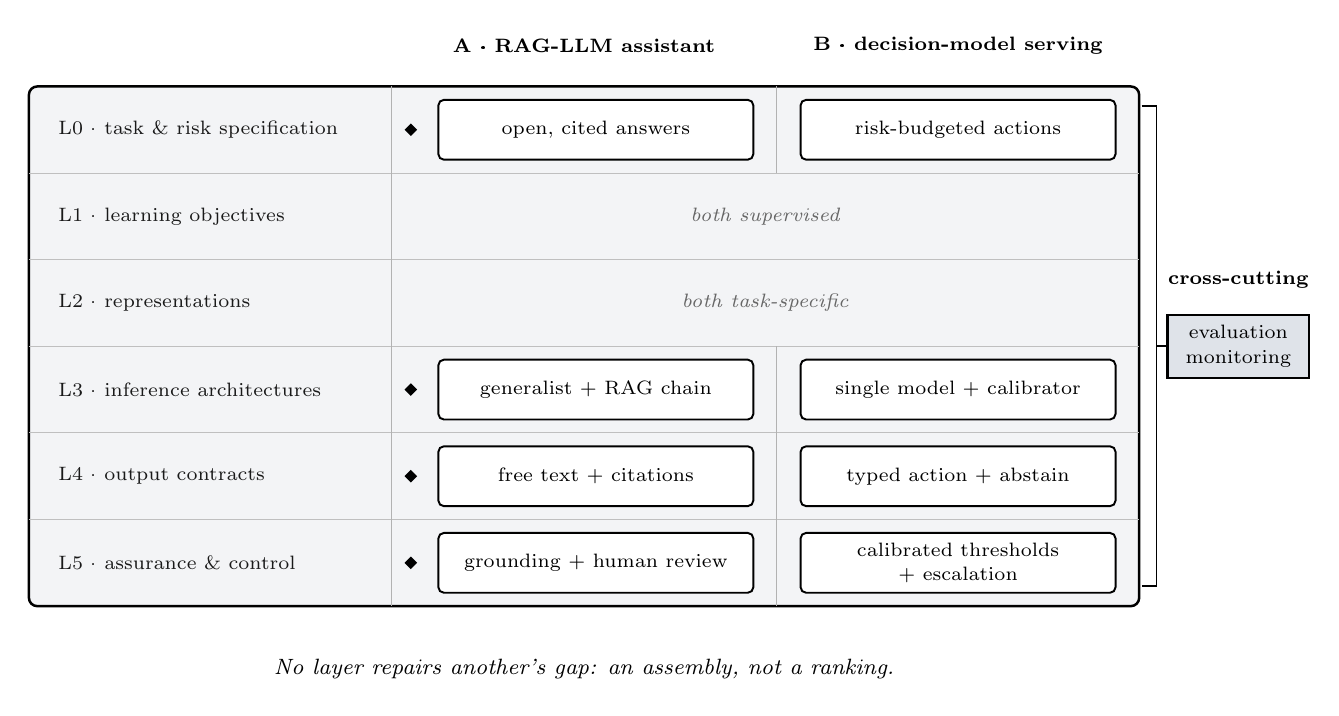
\begin{tikzpicture}[x=1mm,y=1mm]
\tikzset{
  rs/f1chip/.style={rounded corners=2pt, draw=black, line width=0.7pt, fill=white,
    align=center, inner sep=2.2pt, minimum width=40mm, minimum height=7.6mm,
    font=\fontsize{7.5}{8.8}\selectfont},
  rs/f1title/.style={anchor=west, font=\fontsize{7.5}{9.2}\selectfont, text=black!90},
  rs/f1same/.style={anchor=center, font=\fontsize{7.5}{9.0}\selectfont\itshape, text=black!60},
  rs/f1hdr/.style={anchor=center, font=\fontsize{7.5}{9.0}\selectfont\bfseries, text=black},
}
% ===== one continuous stack: tinted frame + row separators + title rule =====
\fill[rsPanelTint, rounded corners=3pt] (0,0) rectangle (141,-66);
\draw[black, line width=0.9pt, rounded corners=3pt] (0,0) rectangle (141,-66);
\foreach \ry in {-11,-22,-33,-44,-55} { \draw[black!25, line width=0.35pt] (0,\ry) -- (141,\ry); }
\draw[black!30, line width=0.35pt] (46,0) -- (46,-66);
% ===== instance headers =====
\node[rs/f1hdr] at (70.5,5.2) {A \textperiodcentered{} RAG-LLM assistant};
\node[rs/f1hdr] at (118,5.2)  {B \textperiodcentered{} decision-model serving};
% ===== layer titles =====
\node[rs/f1title] at (2.5,-5.5)  {L0 \textperiodcentered{} task \& risk specification};
\node[rs/f1title] at (2.5,-16.5) {L1 \textperiodcentered{} learning objectives};
\node[rs/f1title] at (2.5,-27.5) {L2 \textperiodcentered{} representations};
\node[rs/f1title] at (2.5,-38.5) {L3 \textperiodcentered{} inference architectures};
\node[rs/f1title] at (2.5,-49.5) {L4 \textperiodcentered{} output contracts};
\node[rs/f1title] at (2.5,-60.5) {L5 \textperiodcentered{} assurance \& control};
% ===== L0: different kind of specification =====
\node[rs/f1chip] at (72,-5.5)  {open, cited answers};
\node[rs/f1chip] at (118,-5.5) {risk-budgeted actions};
\draw[black!30, line width=0.35pt] (95,-11) -- (95,0);
% ===== L1 / L2: same kind in both instances (no divider, one shared phrase) =====
\node[rs/f1same] at (93.5,-16.5) {both supervised};
\node[rs/f1same] at (93.5,-27.5) {both task-specific};
% ===== L3: different kind of architecture =====
\node[rs/f1chip] at (72,-38.5)  {generalist + RAG chain};
\node[rs/f1chip] at (118,-38.5) {single model + calibrator};
\draw[black!30, line width=0.35pt] (95,-44) -- (95,-33);
% ===== L4: different kind of contract =====
\node[rs/f1chip] at (72,-49.5)  {free text + citations};
\node[rs/f1chip] at (118,-49.5) {typed action + abstain};
\draw[black!30, line width=0.35pt] (95,-55) -- (95,-44);
% ===== L5: same assurance job, different instrument =====
\node[rs/f1chip] at (72,-60.5)  {grounding + human review};
\node[rs/f1chip] at (118,-60.5) {calibrated thresholds\\+ escalation};
\draw[black!30, line width=0.35pt] (95,-66) -- (95,-55);
% ===== divergence marks: 1.6mm filled diamonds in the title gutter =====
\foreach \dy in {-5.5,-38.5,-49.5,-60.5} {
  \fill (48.5,\dy+0.8) -- (49.3,\dy) -- (48.5,\dy-0.8) -- (47.7,\dy) -- cycle;
}
% ===== cross-cutting rail: ONE full-height bracket = acts at every layer =====
\draw[black, line width=0.7pt] (141.3,-2.5) -- (143.2,-2.5) -- (143.2,-63.5) -- (141.3,-63.5);
\draw[black, line width=0.7pt] (143.2,-33) -- (144.6,-33);
\node[anchor=center, inner sep=0pt, font=\fontsize{7.5}{9.0}\selectfont\bfseries, text=black] at (153.6,-24.6)
  {cross-cutting};
\node[rs/gInfra, minimum width=18mm, minimum height=8mm, align=center,
  font=\fontsize{7.5}{9.0}\selectfont] at (153.6,-33) {evaluation\\monitoring};
% ===== the thesis, in one sentence =====
\node[anchor=center, font=\fontsize{8}{9.6}\selectfont\itshape, text=black] at (70.5,-74)
  {No layer repairs another's gap: an assembly, not a ranking.};
\end{tikzpicture}

  \caption{ The \reliabilitystack{} (L0--L5) with two example instances in parallel columns. Layers read top-down, L0 specification to L5 assurance; a choice at any layer constrains what the layers below can deliver. Cells appear only where the two instances choose a different kind of thing, and the diamond marks those four layers; L1--L2 carry one shared phrase because both instances make the same kind of choice there. No layer repairs another's gap: the layers assemble into a stack, and no layer outranks another. Layer cuts and cell placements are an analytic synthesis [J]; instance cells are candidate placements --- column B vendor-reported [V], column A our own reconstructed instance [S]; evaluation + monitoring apply at every layer.}
  \label{fig:stack}
\end{figure}
\FloatBarrier

\section{Layer 1 --- Learning Objectives}\label{sec:objectives}
\label{sec:objectives-cards}
This layer collects the method cards for \emph{how a system is trained}; the shared objective-space map is Table \ref{tab:objspace}, and the four-signal comparison is \cref{fig:signals}.

% ===== P4 DRAFT: section 4 (Layer 1) — first written pass, 2026-10-17 =====
\subsection{An objective-space map: Table 1}
\label{sec:objspace}

\begin{table}[!t]
\centering
\small
\begin{tabular}{@{}p{2.5cm}p{3.2cm}p{3.6cm}p{4.2cm}p{0.9cm}@{}}
\toprule
Family & Modelling principle & Reliability question & Not guaranteed / fails & Ev. \\
\midrule
Autoregressive NLL & next-token conditional prediction & does sequence mastery buy factual + constraint correctness? & fluency $\ne$ grounding; poor calibration; unbounded generation & {[E]} \\
Masked / denoising & corrupt-then-recover & does recovery training build faithful representations? & generation is not the objective; encoder-only scope & {[E]} \\
Diffusion / flow matching, incl. production serving (\S\ref{sec:familycards}) & iterative denoising, learned vector fields & quality--latency--risk trade-off of the sampler? & multi-step cost; variability across samplers; risk is reference-relative & {[T, E]} \\
Energy-based & inference as energy-landscape search (NRGPT) & does a different inference principle change reliability? & small-scale evidence; no superiority vs.\ production AR & {[T, E]} \\
Supervised discrimination & $P(y\,|\,x)$ mapping head & is the mapping stable in deployment? & distribution shift; no ``why''; label-space drift & {[E]} \\
Contrastive (CLIP-class) \cite{radford2021clip} & agreement of matching pairs & does embedding similarity imply semantic correctness? & retrieval errors; OOD embeddings; fine-grained mismatch & {[E]} \\
Latent prediction (JEPA family) & predict target representations in latent space & which structure is recoverable, and does prediction help planning? & \emph{JEPA paradox in language}: authors report conditional-concentration failures on ambiguous text & {[A]} \\
Hierarchical code prediction (NCM-class) & coarse-to-fine multiscale residual VQ codes; all codes per level in parallel & does the tokenizer carry meaning exact enough for downstream checks? & tokenizer-stage substitutions (entities, numerals); codebook compounding: authors' provisional analysis; no released production guard & {[A]} \\
Preference / reward post-training & alignment training on top of an objective & does the reward measure what we want? & reward hacking \cite{gao2022overoptimization}; miscalibrated verifiers \cite{id260601066} & {[E]} \\
Reasoning post-training (RLVR) & policy optimization against a programmatic checker, reusing the AR factorization & does verifier-checkable correctness at training time survive deployment? & verifier gaming \cite{id260601066}, length inflation \cite{id250405185}, coverage loss at large $k$ \cite{id250413837}, unfaithful traces \cite{id230504388}, compute saturation \cite{id261019362} & {[E, A]} \\
\bottomrule
\end{tabular}
\caption{Objective-space map. Each family is optimized for a different currency; no column
is interchangeable. Ev.\ = the class of a row's strongest anchor; where two classes appear, the
first governs. Chips carry the dominant class of the single claim they name; [C]/[N] mark
contradiction and absence; the full alphabet is
\cref{tab:evidence-classes}. Rows are \emph{candidates}; the
selection procedure lives in Section~\ref{sec:selection}.}
\label{tab:objspace}
\end{table}

The first layer of the \reliabilitystack{} asks what a model is trained to be. We treat a
\emph{learning objective} as the pair (training signal, probability factorization): autoregressive
next-token prediction combines a factorization of the joint distribution with a negative-log-likelihood
signal~\cite{vaswani2017attention,kaplan2020scaling,hoffmann2022compute}; a language model's
architecture (mostly Transformer) is a separable choice. Keeping the two apart matters for
reliability claims, because a change of factorization converts an architectural family into a
different objective \cite{mdm2025orderar}, and a change of architecture under a fixed objective
changes failure modes without changing what the signal encourages.

Table~\ref{tab:objspace} maps the ten objective families our review identifies (the two newest
entered while we were drafting: hierarchical code prediction, included because it moves failure
into the tokenizer rather than removing it, and reasoning post-training). The columns
follow the method-card schema of Section~\ref{sec:protocol}: the modelling principle, the
reliability question it inherits, and --- critically --- the properties the objective does
\emph{not} deliver. Our claim throughout is that a strong score on any of these signals is not a
downstream property: likelihood, fidelity, sample quality, calibration and semantic correctness are
different currencies \cite{nichol2021improved,acm2023diffusionsurvey,engreports2025modecollapse}.

Three observations from Table~\ref{tab:objspace} carry through the paper.

\textbf{(i) Transfer:} an objective that works in one modality need not
concentrate its signal for another. The clearest documented case is the JEPA paradox: deterministic
squared-error latent prediction presumes \emph{conditional concentration} of target representations,
which masked text violates because several valid continuations are near-equidistant
\cite{klindt2026lejepa,identifiability2026}. The same caution applies to importing image-era
diffusion assumptions into language: D3PM ties masked-diffusion training to discrete state
spaces~\cite{austin2021d3pm}, recent theory shows those trainers implicitly learn token-order
strategies, i.e.\ a factorization in disguise~\cite{mdm2025orderar}, and controlled generation
arrives only with a redesigned continuous objective~\cite{li2022diffusionlm}.

\textbf{(ii) Historical trade-offs are our thesis in miniature.} GANs optimized realism via
adversarial play and inherited mode collapse and unstable games~\cite{goodfellow2014gan,
arjovsky2017wgan,engreports2025modecollapse}; VAE regularized a latent space and paid with posterior
collapse and blurry samples~\cite{kingma2014vae,higgins2017betavae}; normalizing flows bought exact
likelihood with architectural constraints on capacity~\cite{pmlr2021nf}; flow matching replaced
stochastic diffusion transport with regression along probability paths, separately from any
invertibility constraint~\cite{lipman2023flow}. Each is an instance of our central question ---
\emph{the objective decides what the system cannot deliver} --- long before the scale debate; we
use them as comparative rows (the catalogue genre is
already served, e.g.\ \cite{almuammar2026genai,yazdani2025genaidepth}).

\textbf{(iii) The assurance layer is objective-agnostic and always needed.} Grounding, validators,
calibrated acceptance and escalation (L5) wrap \emph{any} row of Table~\ref{tab:objspace}; the
objective changes only \emph{where} the inherited failures sit; assurance is
needed on every row. The
block-diffusion serving literature is today's cleanest demonstration that an inference
configuration can be chosen against a reference-relative risk budget rather than a mean
benchmark score, and that the same selection procedure transfers, up to precision limits and with
batch-invariant sampling, to speculative-decoding acceptance rules and to weight
quantization~\cite{id260933887} --- the
pattern we generalize in Sections~\ref{sec:contracts}--\ref{sec:assurance}.




\begin{figure}[t]
  \centering
  % \includegraphics[width=\linewidth]{figures/f3_learning_signals.pdf}
  \resizebox{\linewidth}{!}{% figures/f3_learning_signals.tex — F3 v6 (2026-10-19): V4 redesign B2 "stage grid".
% Four objective/signal families as ROWS on one shared four-column stage grid:
%   family [label block] | input -> what is optimized -> prediction target | cannot deliver
% Fixed x columns (50 / 86 / 122), one header row, one heavy header rule: the alignment carries
% the comparison. train: stays a one-line sub-label under the family name; each family's failure
% moves into column 4 (bold = the argument, the only bold text besides family titles).
% D's extra node is folded into a two-cell inset inside column 2 ("shared enc." -> "predictor"),
% so every row has the same three-stage chain.
% Accent: panel (C)'s mechanism chip is the ONE amber = the typed-decision contract, the item the
% ledger defends (threshold-as-policy [V] + independent benchmarking [E]). It is NOT the failure;
% the old caption said so and is wrong (fix logged in docs/caption-pending.md).
% Scope note in the header band: this grid is four training signals, not the ten-family
% objective map (Table 1) -- the old panel grid read as if it were the objective space.
% label: fig:signals   (figure env + \label live in main.tex; F3 slot)
% All in-figure fonts >= 7.5pt; math glyphs set at 8.2pt nominal (CMSY/CMR ~0.92x quirk).
\providecommand{\figsep}{{\fontsize{8.2}{10}\selectfont $|$}}
\providecommand{\figneq}{{\fontsize{8.2}{10}\selectfont $\ne$}}
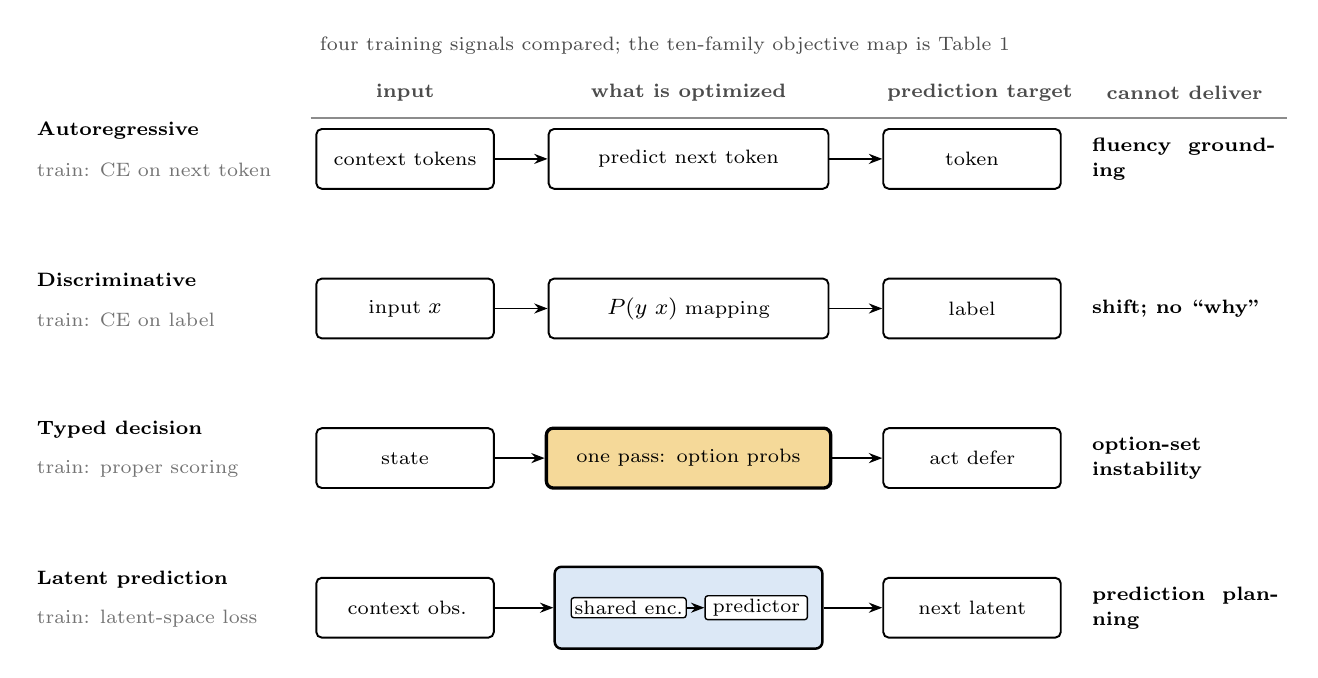
\begin{tikzpicture}[x=1mm,y=1mm]
\tikzset{
  rs/f3cell/.style={rounded corners=2pt, draw=black, line width=0.7pt, fill=white,
    align=center, inner sep=2.2pt, minimum height=7.6mm,
    font=\fontsize{7.5}{8.8}\selectfont},
  rs/f3hdr/.style={anchor=center, font=\fontsize{7.5}{9.0}\selectfont\bfseries, text=black!70},
  rs/f3name/.style={anchor=west, font=\fontsize{7.5}{9.0}\selectfont\bfseries, text=black},
  rs/f3train/.style={anchor=west, font=\fontsize{7.5}{9.0}\selectfont, text=black!55},
  rs/f3fail/.style={anchor=west, align=left, font=\fontsize{7.5}{9.0}\selectfont\bfseries,
    text=black, text width=24mm},
}
% ===== header band: scope note + column names + heavy rule =====
\node[anchor=center, font=\fontsize{7.5}{9.0}\selectfont, text=black!70] at (81,14.4)
  {four training signals compared; the ten-family objective map is Table~1};
\node[rs/f3hdr] at (48,8.4)  {input};
\node[rs/f3hdr] at (84,8.4)  {what is optimized};
\node[rs/f3hdr] at (121,8.4) {prediction target};
\node[rs/f3hdr] at (147,8.4) {cannot deliver};
\draw[black!45, line width=0.6pt] (36,5.2) -- (160,5.2);
% ===== (A) autoregressive =====
\begin{scope}[yshift=0mm]
  \node[rs/f3name] at (0,3.6)  {Autoregressive};
  \node[rs/f3train] at (0,-1.4) {train: CE on next token};
  \node[rs/f3cell, text width=21mm] (a1) at (48,0) {context tokens};
  \node[rs/f3cell, text width=34mm] (a2) at (84,0) {predict next token};
  \node[rs/f3cell, text width=21mm] (a3) at (120,0) {token};
  \draw[rs/gFlow] (a1.east) -- (a2.west); \draw[rs/gFlow] (a2.east) -- (a3.west);
  \node[rs/f3fail] at (134,0) {fluency \figneq\ grounding};
\end{scope}
% ===== (B) discriminative =====
\begin{scope}[yshift=-19mm]
  \node[rs/f3name] at (0,3.6)  {Discriminative};
  \node[rs/f3train] at (0,-1.4) {train: CE on label};
  \node[rs/f3cell, text width=21mm] (b1) at (48,0) {input {\fontsize{8.2}{10}\selectfont $x$}};
  \node[rs/f3cell, text width=34mm] (b2) at (84,0) {{\fontsize{8.2}{10}\selectfont $P(y$\,\figsep\,$x)$} mapping};
  \node[rs/f3cell, text width=21mm] (b3) at (120,0) {label};
  \draw[rs/gFlow] (b1.east) -- (b2.west); \draw[rs/gFlow] (b2.east) -- (b3.west);
  \node[rs/f3fail] at (134,0) {shift; no ``why''};
\end{scope}
% ===== (C) typed decision (the ONE accent = the decision contract) =====
\begin{scope}[yshift=-38mm]
  \node[rs/f3name] at (0,3.6)  {Typed decision};
  \node[rs/f3train] at (0,-1.4) {train: proper scoring};
  \node[rs/f3cell, text width=21mm] (c1) at (48,0) {state};
  \node[rs/gAccent, text width=34mm, minimum height=7.6mm, align=center,
    font=\fontsize{7.5}{8.8}\selectfont] (c2) at (84,0) {one pass: option probs};
  \node[rs/f3cell, text width=21mm] (c3) at (120,0) {act\,\figsep\,defer};
  \draw[rs/gFlow] (c1.east) -- (c2.west); \draw[rs/gFlow] (c2.east) -- (c3.west);
  \node[rs/f3fail] at (134,0) {option-set\\instability};
\end{scope}
% ===== (D) latent prediction: extra encoder folded into a two-cell inset (column 2) =====
\begin{scope}[yshift=-57mm]
  \node[rs/f3name] at (0,3.6)  {Latent prediction};
  \node[rs/f3train] at (0,-1.4) {train: latent-space loss};
  \node[rs/f3cell, text width=21mm] (d1) at (48,0) {context obs.};
  \node[rs/gModel, minimum width=34mm, minimum height=10.4mm, inner sep=0pt] (dc) at (84,0) {};
  \node[draw, rounded corners=1pt, line width=0.5pt, fill=white, inner sep=1.2pt,
    minimum width=14mm, font=\fontsize{7.5}{8.8}\selectfont] (d3) at (76.4,0) {shared enc.};
  \node[draw, rounded corners=1pt, line width=0.5pt, fill=white, inner sep=1.2pt,
    minimum width=13mm, font=\fontsize{7.5}{8.8}\selectfont] (d5) at (92.6,0) {predictor};
  \draw[rs/gFlow] (d3.east) -- (d5.west);
  \node[rs/f3cell, text width=21mm] (d6) at (120,0) {next latent};
  \draw[rs/gFlow] (d1.east) -- (dc.west); \draw[rs/gFlow] (dc.east) -- (d6.west);
  \node[rs/f3fail] at (134,0) {prediction \figneq\ planning};
\end{scope}
\end{tikzpicture}
}
  \caption{ Four training signals on one stage grid --- input, what is optimized, prediction target, and what the signal cannot deliver: autoregressive next-token, supervised discrimination, typed decisions, latent prediction. The amber chip marks the typed-decision mechanism, the item the ledger carries as threshold-as-policy [V] with independent benchmarking [E] (\cref{sec:contracts}); it is a claim, not a failure; each row's failure sits in the last column. The grid compares four signals; the ten-family objective map is Table~\ref{tab:objspace}. Signals and their failures are candidates.}
  \label{fig:signals}
\end{figure}

\subsection{Family cards: objectives, envelopes, complements}
\label{sec:familycards}

We expand the ten Table~\ref{tab:objspace} rows into eight compact cards: what the objective
\emph{optimizes}, where it \emph{excels}, where it \emph{fails}, and which complementary chapters (Sections~\ref{sec:contracts}--\ref{sec:assurance}) cover the residual. Eight cards cover ten rows because discrimination and contrastive learning share one card --- their inherited failure is the same mapping-stability question (Fig.~\ref{fig:fam-contrastive}) --- and latent prediction (JEPA) is argued in prose below and instantiated in Case~4 (\cref{sec:case-jepa}), which is where its envelope becomes measurable. Each card reads left to right --- data in, the training mechanism, the learned object, the output --- with the inherited failure hung below the learned object on a dashed arrow and the training signal in the footer. Cards are
candidates; the selection procedure in \cref{sec:selection} consumes them.

\paragraph{Autoregressive next-token prediction.}
\noindent The mechanism is sketched in \cref{fig:fam-ar}.

\begin{figure}[t]\centering
  \resizebox{\linewidth}{!}{% figures/f_fam_ar.tex — Family-card sketch: autoregressive next-token prediction (Table 1 row 1).
% Grammar: figures/style_v2_tokens.tex (v8 token grammar). Roles: payload = rs/gData (rounded
%   green); training mechanism + learned object = rs/gModel (rounded blue); the inherited-failure
%   box = rs/gAccent (the ONE yellow = ledger-defended item); dashed edge = claim-to-defend.
% Chain: token stream under a causal mask -> next-token NLL trainer -> learned conditional LM ->
%   token-by-token text at inference.
% Accent (yellow): the inherited failure the claim ledger documents [E] — fluency is not
%   grounding; calibration does not ride on the likelihood signal.
% label: fig:fam-ar   (figure env + \label live in the family-cards slot of main.tex; parent wires)
%
% CAPTION NOTE — items the paper must defend:
%   1. [E] fluency != grounding: hallucination surveys report persistent inconsistency across
%      elicitation formats (id251006265 in the card); no figure carries a rate;
%   2. calibration is not guaranteed out of the box — the case-study packs cite this per system,
%      not per family; box line 2 carries [A] (per-system report), not a family-level [E];
%   3. complements are named, not measured: retrieval, contracts, acceptance (L4--L5) carry the
%      residual; composition effects stay [GAP].
% Fonts >= 7.5pt; math glyphs measure ~0.92x nominal (CMSY/CMR quirk) so symbols use 8.2pt.
\providecommand{\figsep}{{\fontsize{8.2}{10}\selectfont $|$}}
\providecommand{\figneq}{{\fontsize{8.2}{10}\selectfont $\ne$}}
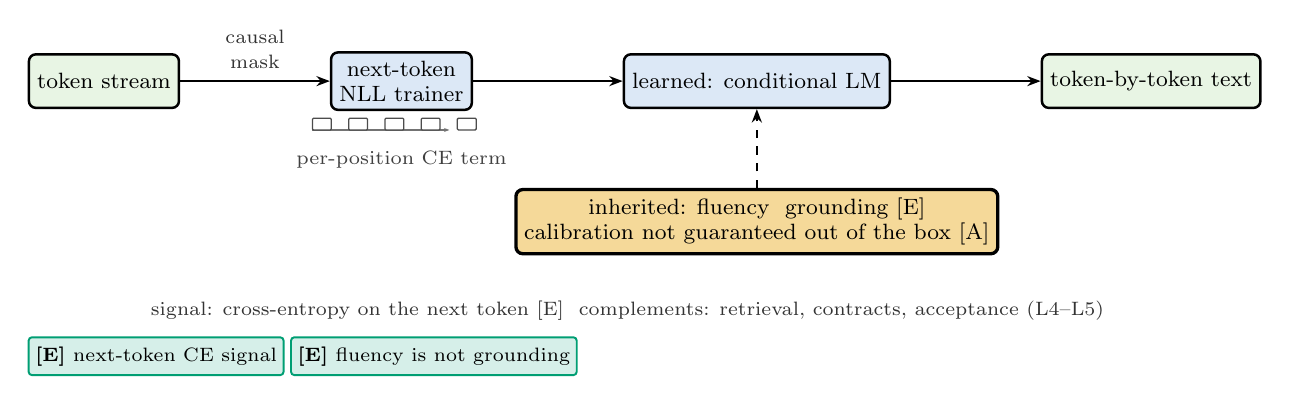
\begin{tikzpicture}
% ===== chain (training signal -> learned object -> inference output) =====
\node[rs/gData] (tok) {token stream};
\node[rs/gModel, right=19mm of tok] (nll) {next-token\\NLL trainer};
\node[rs/gModel, right=19mm of nll] (lm) {learned: conditional LM};
\node[rs/gData, right=19mm of lm] (gen) {token-by-token text};
% ===== causal-mask annotation on the signal edge (4mm lift: matches the other family cards) =====
\coordinate (emid) at ($(tok.east)!0.5!(nll.west)$);
\node[rs/gEdgeLbl, align=center] at ([yshift=4mm]emid) {causal\\mask};
% ===== inherited failure (yellow = ledger-defended item) =====
\node[rs/gAccent, below=10mm of lm] (fail) {inherited: fluency \figneq\ grounding [E]\\calibration not guaranteed out of the box [A]};
% ===== edges =====
\draw[rs/gFlow] (tok.east) -- (nll.west);
\draw[rs/gFlow] (nll.east) -- (lm.west);
\draw[rs/gFlow] (lm.east) -- (gen.west);
\draw[rs/gFlowD] (fail.north) -- (lm.south);
% ===== foot =====
\coordinate (mid) at ($(tok.center)!0.5!(gen.center)$);
\node[rs/gFoot] at ([yshift=-7mm]mid |- fail.south) {signal: cross-entropy on the next token [E] \figsep\ complements: retrieval, contracts, acceptance (L4--L5)};
% --- loss tape (P3): the signal structure this card's trainer consumes: one term per position, in order
\rsLossTape{ar}{nll.south}{-2.4mm}{per-position CE term}
% --- evidence ribbon (P2): segments are claims already carried above; tag = the claim's class.
\rsRibbonBase{-3.4mm}
\rsRibbonRow{0mm}
\rsRibSeg{rsVerified}{\textbf{[E]} next-token CE signal}
\rsRibSeg{rsVerified}{\textbf{[E]} fluency is not grounding}
\end{tikzpicture}
}
  \caption{Family card: autoregressive next-token prediction. Yellow = the inherited failure with the strongest ledger support.}
  \label{fig:fam-ar}
\end{figure}

\textit{Optimizes} conditional sequence likelihood (left-to-right factorization over the joint, NLL signal); compute scaling follows observed
laws~\cite{kaplan2020scaling,hoffmann2022compute}. \textit{Excels at} open-ended generation,
in-context adaptation, and tool-readable instruction following --- the substrate every layer
above assumes. \textit{Fails at} factual guarantees (fluency is not truth; hallucination
surveys report persistent inconsistency across elicitation formats
~\cite{id251006265}) and calibration out of the box. \textit{Complements:} retrieval
grounding, output contracts, calibrated acceptance and escalation (\S\ref{sec:contracts}--\S\ref{sec:assurance}).

\paragraph{Masked and denoising objectives.}
\noindent The mechanism is sketched in \cref{fig:fam-masked}.

\begin{figure}[t]\centering
  \resizebox{\linewidth}{!}{% figures/f_fam_masked.tex — Family-card sketch: masked / denoising objectives (Table 1 row 2).
% Grammar: figures/style_v2_tokens.tex (v8 token grammar). Roles: payload = rs/gData;
%   mechanism + learned object = rs/gModel; inherited-failure box = rs/gAccent (the ONE yellow).
% Chain: text -> corruption (mask spans) as the training signal -> recovery trainer -> learned
%   bidirectional encoder -> contextual embeddings at inference.
% Accent (yellow): the inherited failure the claim ledger documents [E] — generation is not the
%   training signal; sampling is not defined by the trainer (D3PM contrast in the foot line).
% label: fig:fam-masked   (figure env + \label live in the family-cards slot of main.tex; parent wires)
%
% CAPTION NOTE — items the paper must defend:
%   1. [E] recovery training targets representations, not a generator (austin2021d3pm,
%      mdm2025orderar in the card); "encoder-only scope" is the card's phrase;
%   2. D3PM contrast: the same corruption family splits into representation-trainers and
%      sequence-generators only when sampling is defined — the vicinity arrow is dashed for
%      exactly this claim;
%   3. no mask-rate number appears in the figure by design (reference-free labels only).
% Fonts >= 7.5pt; math glyphs measure ~0.92x nominal (CMSY/CMR quirk) so symbols use 8.2pt.
\providecommand{\figsep}{{\fontsize{8.2}{10}\selectfont $|$}}
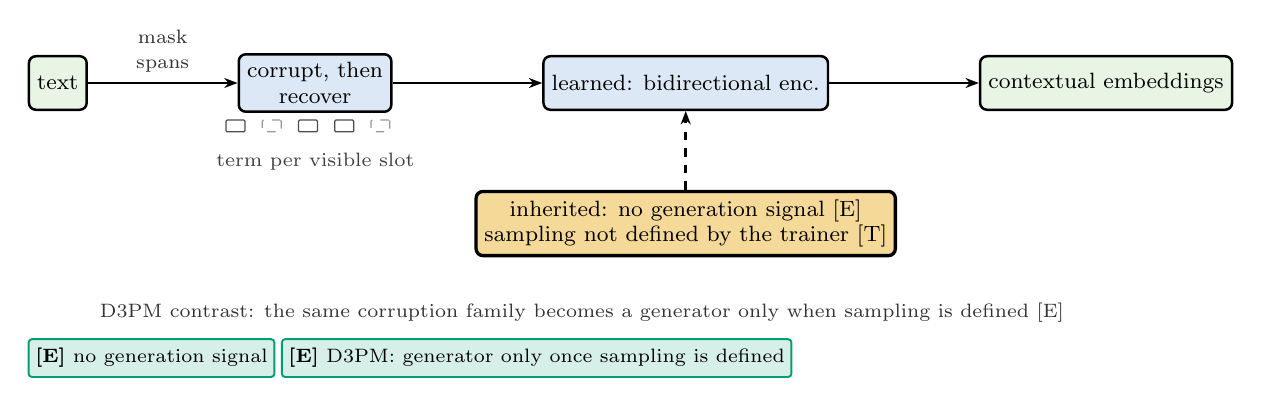
\begin{tikzpicture}
% ===== chain =====
\node[rs/gData] (txt) {text};
\node[rs/gModel, right=19mm of txt] (mrec) {corrupt, then\\recover};
\node[rs/gModel, right=19mm of mrec] (enc) {learned: bidirectional enc.};
\node[rs/gData, right=19mm of enc] (emb) {contextual embeddings};
% ===== corruption annotation on the signal edge (4mm lift: matches the other family cards) =====
\coordinate (emid) at ($(txt.east)!0.5!(mrec.west)$);
\node[rs/gEdgeLbl, align=center] at ([yshift=4mm]emid) {mask\\spans};
% ===== inherited failure (yellow = ledger-defended item) =====
\node[rs/gAccent, below=10mm of enc] (fail) {inherited: no generation signal [E]\\sampling not defined by the trainer [T]};
% ===== edges =====
\draw[rs/gFlow] (txt.east) -- (mrec.west);
\draw[rs/gFlow] (mrec.east) -- (enc.west);
\draw[rs/gFlow] (enc.east) -- (emb.west);
\draw[rs/gFlowD] (fail.north) -- (enc.south);
% ===== foot =====
\coordinate (mid) at ($(txt.center)!0.5!(emb.center)$);
\node[rs/gFoot] at ([yshift=-7mm]mid |- fail.south) {D3PM contrast: the same corruption family becomes a generator only when sampling is defined [E]};
% --- loss tape (P3): a bag of per-position terms; only visible targets carry one
\rsLossTape{masked}{mrec.south}{-2.4mm}{term per visible slot}
% --- evidence ribbon (P2): segments are claims already carried above; tag = the claim's class.
\rsRibbonBase{-3.4mm}
\rsRibbonRow{0mm}
\rsRibSeg{rsVerified}{\textbf{[E]} no generation signal}
\rsRibSeg{rsVerified}{\textbf{[E]} D3PM: generator only once sampling is defined}
\end{tikzpicture}
}
  \caption{Family card: masked / denoising objectives.}
  \label{fig:fam-masked}
\end{figure}

\textit{Optimizes} recovery from corruptions; trains representations that transfer broadly.
\textit{Excels at} encoder tasks and representation learning with modest data.
\textit{Fails at} generation: the training signal is recovery, and the D3PM contrast with
masked-diffusion generation shows the same corruption family splits into
representation-trainers and sequence-generators only when sampling is defined
~\cite{austin2021d3pm,mdm2025orderar}. \textit{Complements:} pair with a decoding layer or
use as the base for specialist encoders.

\paragraph{Diffusion and flow matching.}
\noindent The mechanism is sketched in \cref{fig:fam-diffusion}.

\begin{figure}[t]\centering
  \resizebox{\linewidth}{!}{% figures/f_fam_diffusion.tex — Family-card sketch: diffusion / flow matching (Table 1 row 3).
% Grammar: figures/style_v2_tokens.tex (v8 token grammar). Roles: payload = rs/gData;
%   mechanism / learned field / sampler = rs/gModel; inherited-failure box = rs/gAccent (ONE yellow).
% Chain: noise -> iterative denoising (t = T -> 0) -> learned score / velocity field ->
%   sampler choice -> sample at inference.
% Accent (yellow): the inherited failure the claim ledger documents [T,E] — sampler sensitivity:
%   the same trainer yields different samples across samplers.
% label: fig:fam-diffusion   (figure env + \label live in the family-cards slot of main.tex; parent wires)
%
% CAPTION NOTE — items the paper must defend:
%   1. [T,E] sampler sensitivity: same trainer, different samplers, different samples
%      (song2021ddim in the card); the comprehensive survey documents
%      likelihood-vs-sample-quality separations (acm2023diffusionsurvey);
%   2. the flow-matching contrast (lipman2023flow) is a family VARIANT — regression along
%      probability paths — not a separate row of the table;
%   3. no sampler name is endorsed in the figure; sampler choice is an assurance question
%      (risk-budgeted serving, section 5) not a benchmark answer.
% Fonts >= 7.5pt; math glyphs measure ~0.92x nominal (CMSY/CMR quirk) so symbols use 8.2pt.
\providecommand{\figtT}{{\fontsize{8.2}{10}\selectfont $t = T$}}
\providecommand{\figtoz}{{\fontsize{8.2}{10}\selectfont $\to 0$}}
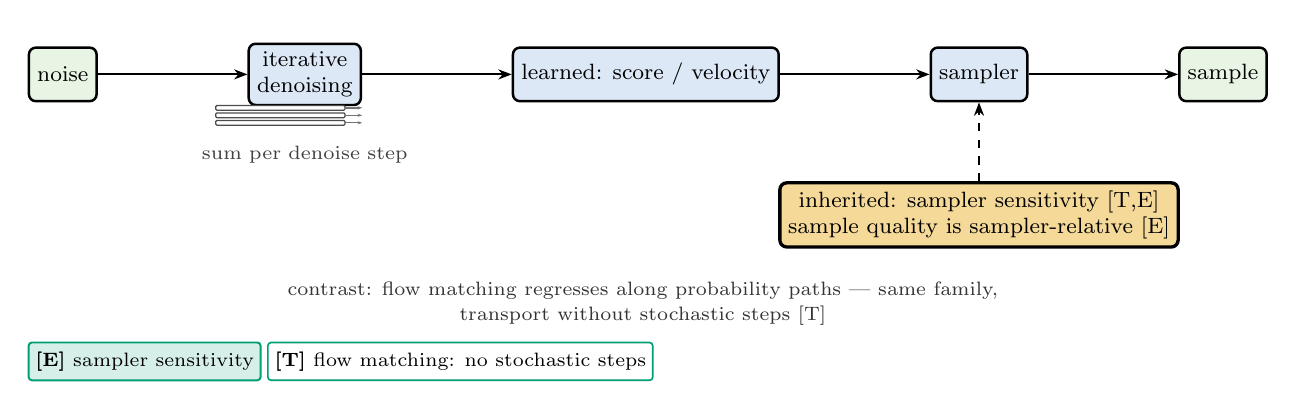
\begin{tikzpicture}
% ===== chain =====
\node[rs/gData] (noi) {noise};
\node[rs/gModel, right=19mm of noi] (den) {iterative\\denoising};
\node[rs/gModel, right=19mm of den] (fld) {learned: score / velocity};
\node[rs/gModel, right=19mm of fld] (smp) {sampler};
\node[rs/gData, right=19mm of smp] (smpo) {sample};
% ===== step-direction annotation on the signal edge (4mm lift: matches the other family cards) =====
\coordinate (emid) at ($(noi.east)!0.5!(den.west)$);
\node[rs/gEdgeLbl, align=center] at ([yshift=4mm]emid) {\figtT\\\figtoz};
% ===== inherited failure (yellow = ledger-defended item) =====
\node[rs/gAccent, below=10mm of smp] (fail) {inherited: sampler sensitivity [T,E]\\sample quality is sampler-relative [E]};
% ===== edges =====
\draw[rs/gFlow] (noi.east) -- (den.west);
\draw[rs/gFlow] (den.east) -- (fld.west);
\draw[rs/gFlow] (fld.east) -- (smp.west);
\draw[rs/gFlow] (smp.east) -- (smpo.west);
\draw[rs/gFlowD] (fail.north) -- (smp.south);
% ===== foot =====
\coordinate (mid) at ($(noi.center)!0.5!(smpo.center)$);
\node[rs/gFoot] at ([yshift=-7mm]mid |- fail.south) {contrast: flow matching regresses along probability paths --- same family,\\transport without stochastic steps [T]};
% --- loss tape (P3): one summed term per denoise step, over the whole sequence
\rsLossTape{diffusion}{den.south}{-2.4mm}{sum per denoise step}
% --- evidence ribbon (P2): segments are claims already carried above; tag = the claim's class.
\rsRibbonBase{-3.4mm}
\rsRibbonRow{0mm}
\rsRibSeg{rsVerified}{\textbf{[E]} sampler sensitivity}
\rsRibSeg{rsTheory}{\textbf{[T]} flow matching: no stochastic steps}
\end{tikzpicture}
}
  \caption{Family card: diffusion and flow matching (sampler sensitivity as the inherited failure).}
  \label{fig:fam-diffusion}
\end{figure}

\textit{Optimizes} iterative denoising (DDPM; improved variants tie likelihood to
FID-style diversity \cite{ho2020ddpm,nichol2021improved}) or regression along probability paths
\cite{lipman2023flow}; discrete state spaces and controllable formulations carry these into
text \cite{austin2021d3pm,li2022diffusionlm}, with parallel-decoding latency arguments spanning
the DLM survey~\cite{zhan2025dlmsurvey}, Turkish masked-diffusion proof-of-concept
 Diffutron~\cite{id260320466}, and order-learning bridges~\cite{mdm2025orderar}.
\textit{Fails at} sampler sensitivity: the same trainer yields different samples across samplers
(DDIM \cite{song2021ddim}); the comprehensive survey documents likelihood-vs-sample-quality separations
\cite{acm2023diffusionsurvey}. \textit{Complements:} risk-budgeted serving (\S\ref{sec:l5-calibrated}) turns
sampler choice into an assurance question rather than a benchmark answer.

\paragraph{Energy-based objectives.}
\noindent The mechanism is sketched in \cref{fig:fam-energy}.

\begin{figure}[t]\centering
  \resizebox{\linewidth}{!}{% figures/f_fam_energy.tex — Family-card sketch: energy-based objectives (Table 1 row 4).
% Grammar: figures/style_v2_tokens.tex (GRAY claim box = cards-pack [GAP] style, not the yellow accent).
% Chain: context -> inference as search over an energy landscape -> learned energy E -> searched
%   minima as outputs (search, not one-pass decoding).
% Accent (GRAY, deliberately not yellow): the inherited failure is an honest-null row — no
%   quantitative anchor; scale evidence remains small; no superiority over production AR.
% label: fig:fam-energy   (figure env + \label live in the family-cards slot of main.tex; parent wires)
%
% CAPTION NOTE — items the paper must defend:
%   1. [GAP] no quantitative anchor: demonstrations remain small and no superiority over
%      production AR systems is established in our evidence base — state this as the null, not
%      as a performance claim;
%   2. the mechanism itself is [T]: an energy landscape whose minima are plausible outputs
%      (NRGPT class, card text); inference is search, not one-pass decoding;
%   3. value today is conceptual (tunable search effort), not deployed reliability — the usual
%      assurance stack applies unchanged.
% Fonts >= 7.5pt; math glyphs measure ~0.92x nominal (CMSY/CMR quirk) so symbols use 8.2pt.
\providecommand{\figsep}{{\fontsize{8.2}{10}\selectfont $|$}}
\providecommand{\figeq}{{\fontsize{8.2}{10}\selectfont $=$}}
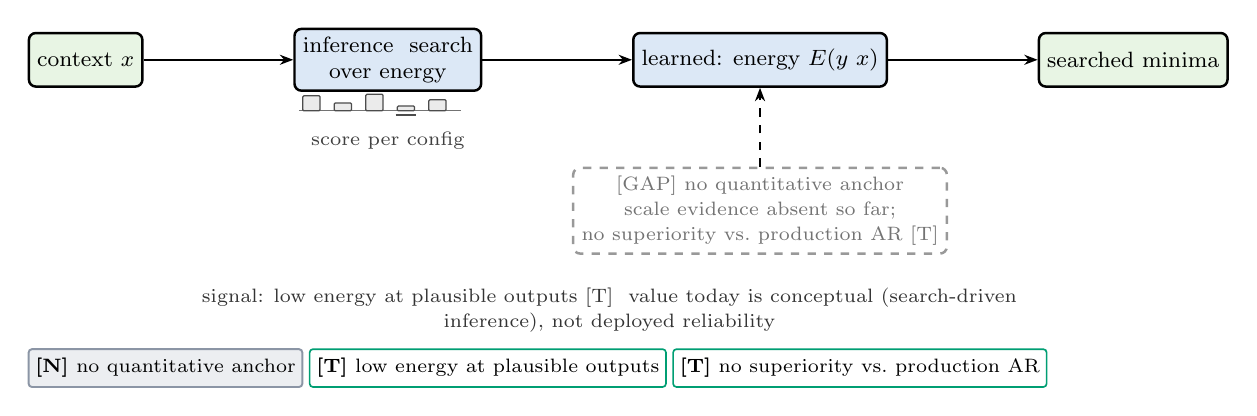
\begin{tikzpicture}
\tikzset{rs/famGap/.style={rounded corners=2.5pt, draw=black!40, line width=0.9pt, dashed,
  fill=white, align=center, inner sep=3pt, font=\fontsize{7.5}{9.0}\selectfont, text=black!55}}
% ===== chain =====
\node[rs/gData] (ctx) {context $x$};
\node[rs/gModel, right=19mm of ctx] (srch) {inference \figeq\ search\\over energy};
\node[rs/gModel, right=19mm of srch] (nrg) {learned: energy $E(y$\,\figsep\,$x)$};
\node[rs/gData, right=19mm of nrg] (min) {searched minima};
% ===== inherited failure (GRAY = [GAP]: no quantitative anchor) =====
\node[rs/famGap, below=10mm of nrg] (gap) {[GAP] no quantitative anchor\\scale evidence absent so far;\\no superiority vs.\ production AR [T]};
% ===== edges =====
\draw[rs/gFlow] (ctx.east) -- (srch.west);
\draw[rs/gFlow] (srch.east) -- (nrg.west);
\draw[rs/gFlow] (nrg.east) -- (min.west);
\draw[rs/gFlowD] (gap.north) -- (nrg.south);
% ===== foot =====
\coordinate (mid) at ($(ctx.center)!0.5!(min.center)$);
\node[rs/gFoot] at ([yshift=-7mm]mid |- gap.south) {signal: low energy at plausible outputs [T] \figsep\ value today is conceptual (search-driven\\inference), not deployed reliability};
% --- loss tape (P3): one score term per candidate configuration; the minimum is the output
\rsLossTape{energy}{srch.south}{-2.4mm}{score per config}
% --- evidence ribbon (P2): segments are claims already carried above; tag = the claim's class.
\rsRibbonBase{-3.4mm}
\rsRibbonRow{0mm}
\rsRibSeg{rsNoClaim}{\textbf{[N]} no quantitative anchor}
\rsRibSeg{rsTheory}{\textbf{[T]} low energy at plausible outputs}
\rsRibSeg{rsTheory}{\textbf{[T]} no superiority vs.\ production AR}
\end{tikzpicture}
}
  \caption{Family card: energy-based objectives. Gray = absent evidence ([N]): no quantitative anchor in our ledger; the card's [GAP] label marks the specific unmeasured link behind that absence, not a second finding.}
  \label{fig:fam-energy}
\end{figure}

\textit{Optimizes} an energy landscape whose minima are plausible outputs (NRGPT
class~\cite{nrgpt2025}, [T]);
inference is an iterative search. \textit{Excels at} making inference a tunable
computation, in principle aligning effort with difficulty. \textit{Fails at} scale evidence:
demonstrations remain small; no superiority over production AR systems is established, and we
flag this as an honest open row rather than a case for exclusion. \textit{Complements:} the usual
assurance stack applies; value today is conceptual (search-driven inference).

\paragraph{Discriminative and contrastive representation objectives.}
\noindent The mechanism is sketched in \cref{fig:fam-contrastive}.

\begin{figure}[t]\centering
  \resizebox{\linewidth}{!}{% figures/f_fam_contrastive.tex — Family-card sketch: contrastive (CLIP-class) objectives (Table 1 row 6).
% SCOPE: this card draws Table 1 row 6 ONLY. Row 5 (supervised discrimination) shares this card's
%   reliability question but not its mechanism (no P(y|x) head, no label box is drawn); its envelope
%   — label-space drift under shift — is carried by the L4 contract discussion. The caption must
%   therefore read "contrastive", not "discriminative / contrastive" (see changelog handoff).
% Grammar: figures/style_v2_tokens.tex (v8 token grammar). Roles: payload = rs/gData;
%   encoders / learned space = rs/gModel; inherited-failure box = rs/gAccent (the ONE yellow).
% Chain: paired inputs (inputs, matched pair) -> paired encoders -> agreement trainer
%   (pull matching pairs together) -> learned embedding space -> similarity / retrieval at inference.
% Accent (yellow): the inherited failure the claim ledger documents [E] — embedding similarity
%   is not semantic correctness; embeddings are not calibrated probabilities.
% label: fig:fam-contrastive   (figure env + \label live in the family-cards slot of main.tex; parent wires)
%
% CAPTION NOTE — items the paper must defend:
%   1. [E] agreement of matching pairs is the objective's currency; similarity != semantic
%      correctness (retrieval errors, OOD embeddings, fine-grained mismatch — card text);
%   2. [E] embeddings are not calibrated probabilities: threshold policies built directly on
%      embeddings break (this feeds the L4 contract discussion in section 5);
%   3. two-input geometry mirrors F3 panel D; both inputs are wired to the paired encoders.
% Fonts >= 7.5pt; math glyphs measure ~0.92x nominal (CMSY/CMR quirk) so symbols use 8.2pt.
% Notation note: the old $a^+$ superscript is spelled "matched pair" (a superscript glyph would
% publish below the 7pt floor); semantics unchanged.
\providecommand{\figneq}{{\fontsize{8.2}{10}\selectfont $\ne$}}
\providecommand{\figsep}{{\fontsize{8.2}{10}\selectfont $|$}}
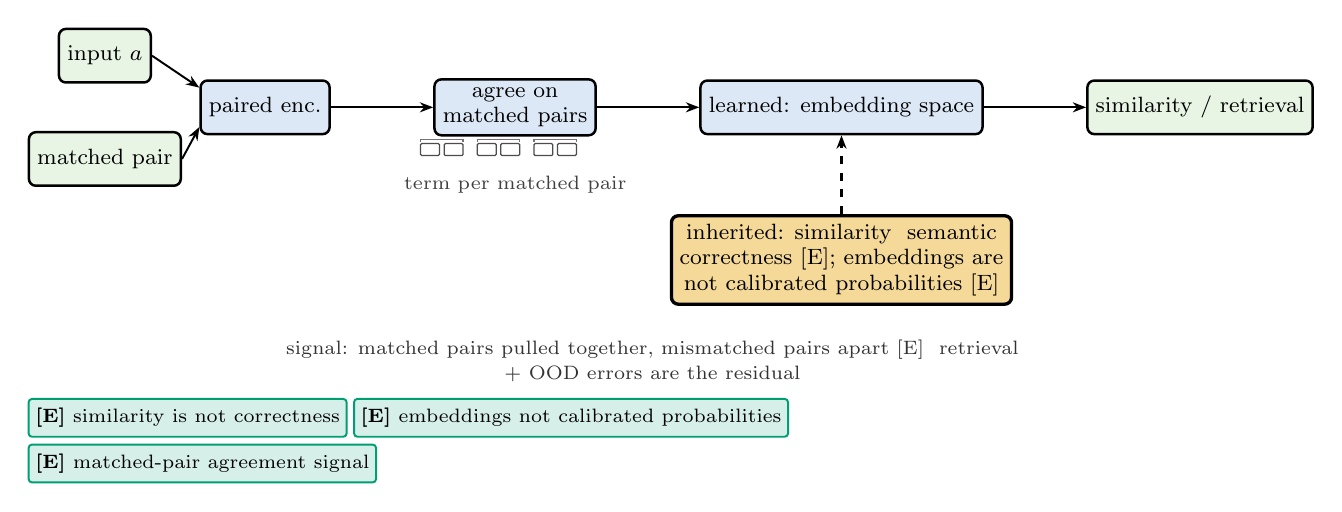
\begin{tikzpicture}
% ===== paired inputs (relative placement: bare coordinates are cm, never mm) =====
\node[rs/gData] (anc) {input $a$};
\node[rs/gData, below=6mm of anc] (pos) {matched pair};
\coordinate (inmid) at ($(anc.center)!0.5!(pos.center)$);
% ===== chain =====
\node[rs/gModel, right=12mm of inmid] (enc) {paired enc.};
\node[rs/gModel, right=13mm of enc] (agr) {agree on\\matched pairs};
\node[rs/gModel, right=13mm of agr] (emb) {learned: embedding space};
\node[rs/gData, right=13mm of emb] (sim) {similarity / retrieval};
% ===== inherited failure (yellow = ledger-defended item) =====
\node[rs/gAccent, below=10mm of emb] (fail) {inherited: similarity \figneq\ semantic\\correctness [E]; embeddings are\\not calibrated probabilities [E]};
% ===== edges (author sweep: the old corner->anchor routing ran the shafts tangent to the
% encoder's top/bottom borders; now both inputs fan into the encoder's LEFT edge) =====
\draw[rs/gFlow] (anc.east) -- ([yshift=2.5mm]enc.west);
\draw[rs/gFlow] (pos.east) -- ([yshift=-2.5mm]enc.west);
\draw[rs/gFlow] (enc.east) -- (agr.west);
\draw[rs/gFlow] (agr.east) -- (emb.west);
\draw[rs/gFlow] (emb.east) -- (sim.west);
\draw[rs/gFlowD] (fail.north) -- (emb.south);
% ===== foot =====
\coordinate (mid) at ($(inmid)!0.5!(sim.center)$);
\node[rs/gFoot] at ([yshift=-7mm]mid |- fail.south) {signal: matched pairs pulled together, mismatched pairs apart [E] \figsep\ retrieval\\+ OOD errors are the residual};
% --- loss tape (P3): terms arrive as pairs, one per matched pair
\rsLossTape{contrastive}{agr.south}{-2.4mm}{term per matched pair}
% --- evidence ribbon (P2): segments are claims already carried above; tag = the claim's class.
\rsRibbonBase{-3.4mm}
\rsRibbonRow{0mm}
\rsRibSeg{rsVerified}{\textbf{[E]} similarity is not correctness}
\rsRibSeg{rsVerified}{\textbf{[E]} embeddings not calibrated probabilities}
\rsRibbonRow{-5.8mm}
\rsRibSeg{rsVerified}{\textbf{[E]} matched-pair agreement signal}
\end{tikzpicture}
}
  \caption{Family card: contrastive representation objectives (Table 1 rows 5--6 --- the supervised-discrimination family shares this row's computed-agreement signal; its own row lives in \cref{tab:objspace}).}
  \label{fig:fam-contrastive}
\end{figure}

\textit{Optimizes} a mapping head or agreement of pairs; typically the cheapest, most
auditable family. \textit{Excels at} narrow, well-instrumented decision regimes where OOD
-monitoring and calibration methods have matured (\S\ref{sec:assurance} cites the UQ
 surveys~\cite{id250315850,id240718418}). \textit{Fails at} open-ended tasks and
distribution shift; embeddings are not calibrated probabilities and break
threshold policies built on them. \textit{Complements:} acceptance/escalation
machinery, designed jointly with the L4 contract.

\paragraph{Latent-predictive joint-embedding objectives (JEPA family).}
\textit{Optimizes} predictability of target representations under partial context
(I-JEPA lineage; the identifiability gap we treat as open in \cref{sec:l2-jepa}
\cite{klindt2026lejepa}). \textit{Excels at} vision-style regimes where the objective matches the
data's structure; attractive because prediction concentrates signal without generative cost.
\textit{Fails at} language: the paradox thesis is that ambiguous-text targets lack
concentration, so squared-error training degrades \cite{identifiability2026};
assumption conditions (e.g.\ non-Gaussian identifiability lifts \cite{id260612471}) remain
unclosed in production settings. \textit{Complements:} world-model planners need an output
contract (\S\ref{sec:contracts}) and monitors (\S\ref{sec:assurance}) exactly because prediction
quality alone does not certify planning quality.

\paragraph{Preference, reward and rule-grounded post-training.}
\noindent The mechanism is sketched in \cref{fig:fam-preference}.

\begin{figure}[t]\centering
  \resizebox{\linewidth}{!}{% figures/f_fam_preference.tex — Family-card sketch: preference / reward post-training (Table 1 row 8).
% Grammar: figures/style_v2_tokens.tex (v8 token grammar). Roles: payload = rs/gData;
%   post-training layer / verifier = rs/gModel; inherited-failure box = rs/gAccent (ONE yellow).
% Chain: base objective -> preference / reward post-training layer -> reward model / verifier
%   (proper scoring rules) -> post-trained policy at inference; the preference signal
%   (rankings / verifiable rules) enters the verifier from above.
% Accent (yellow): the inherited failure the claim ledger documents [E,V] — reward hacking
%   (the signal measures the reward model's beliefs, not ground truth) and a contested
%   calibration direction across independent reproductions, reported as unresolved.
% label: fig:fam-preference   (figure env + \label live in the family-cards slot of main.tex; parent wires)
%
% CAPTION NOTE — items the paper must defend:
%   1. [E] reward hacking: the signal reflects the reward model's beliefs, not ground truth
%      (id260937647 in the card);
%   2. [E,V] calibration direction contested, not resolved — cite per checkpoint, never per
%      family (section 5 carries the measured-direction caveat);
%   3. [V] proper scoring rules are the RLCD / Laya-lineage recipe (vendor-reported), not an
%      independent measurement;
%   4. the layer sits on ANY base objective (row 1 chains it over the base block).
% Fonts >= 7.5pt; math glyphs measure ~0.92x nominal (CMSY/CMR quirk) so symbols use 8.2pt.
\providecommand{\figsep}{{\fontsize{8.2}{10}\selectfont $|$}}
\providecommand{\figneq}{{\fontsize{8.2}{10}\selectfont $\ne$}}
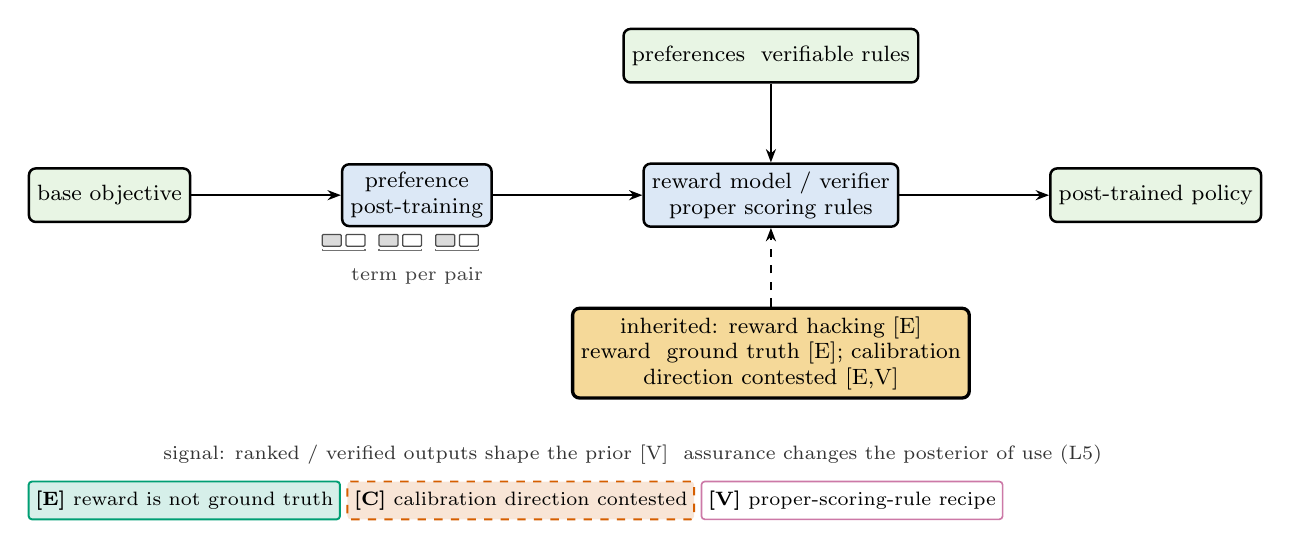
\begin{tikzpicture}
% ===== chain =====
\node[rs/gData] (base) {base objective};
\node[rs/gModel, right=19mm of base] (post) {preference\\post-training};
\node[rs/gModel, right=19mm of post] (ver) {reward model / verifier\\proper scoring rules};
\node[rs/gData, right=19mm of ver] (pol) {post-trained policy};
% ===== preference signal (enters the verifier) =====
\node[rs/gData, above=10mm of ver] (sig) {preferences \figsep\ verifiable rules};
% ===== inherited failure (yellow = ledger-defended item) =====
\node[rs/gAccent, below=10mm of ver] (fail) {inherited: reward hacking [E]\\reward \figneq\ ground truth [E]; calibration\\direction contested [E,V]};
% ===== edges =====
\draw[rs/gFlow] (base.east) -- (post.west);
\draw[rs/gFlow] (post.east) -- (ver.west);
\draw[rs/gFlow] (ver.east) -- (pol.west);
\draw[rs/gFlow] (sig.south) -- (ver.north);
\draw[rs/gFlowD] (fail.north) -- (ver.south);
% ===== foot =====
\coordinate (mid) at ($(base.center)!0.5!(pol.center)$);
\node[rs/gFoot] at ([yshift=-7mm]mid |- fail.south) {signal: ranked / verified outputs shape the prior [V] \figsep\ assurance changes the posterior of use (L5)};
% --- loss tape (P3): one chosen/rejected term pair per preference pair
\rsLossTape{preference}{post.south}{-2.4mm}{term per pair}
% --- evidence ribbon (P2): segments are claims already carried above; tag = the claim's class.
\rsRibbonBase{-3.4mm}
\rsRibbonRow{0mm}
\rsRibSeg{rsVerified}{\textbf{[E]} reward is not ground truth}
\rsRibSeg[dashed]{rsContested}{\textbf{[C]} calibration direction contested}
\rsRibSeg{rsVendor}{\textbf{[V]} proper-scoring-rule recipe}
\end{tikzpicture}
}
  \caption{Family card: preference / reward post-training (contested calibration direction named).}
  \label{fig:fam-preference}
\end{figure}

\textit{Optimizes} alignment of outputs to explicit preferences or verifiable rules on top of
any base objective (RLHF/DPO families; the Laya-class recipe trains decision heads with proper scoring
rules~\evvendor{}; the Jev-class System-One benchmark family shows decision-model
serving gains \cite{rauk2026jevbenchmark}). \textit{Excels at} instilling response shape
and typed decision distributions without re-architecting. \textit{Fails at} reward hacking and
miscalibrated verifiers: the signal reflects the reward model's beliefs, not ground truth
\cite{gao2022overoptimization,id260601066}; direction-of-miscalibration disagreements across independent reproductions
are documented for the Laya-class architecture and reported as contested and unresolved
(\S\ref{sec:contracts}). \textit{Complements:} The entire L5 stack; post-training changes the
prior, assurance changes the posterior of use.

\paragraph{Reasoning post-training (RLVR).}
\noindent The mechanism is sketched in \cref{fig:fam-reasoning}.

\begin{figure}[t]\centering
  \resizebox{\linewidth}{!}{% figures/f_fam_reasoning.tex — Family card: reasoning post-training / RLVR (Table 1 row 10).
% Grammar: figures/style_v2_tokens.tex (v8 token grammar). Roles: problem+key and the selected
%   trajectory = rs/gData; policy and its rollout group = rs/gModel; the programmatic checker =
%   rs/gControl (amber octagon — the grammar reserves the octagon for a gate that stops flow);
%   the inherited-failure strip = rs/gAccent (the ONE yellow); edges rs/gFlow / rs/gFlowD.
% Chain: verifiable problem -> policy rollouts -> programmatic checker -> selected trajectory.
%   The dashed loop above the chain is the TEST-TIME pass (resample N, keep the checker's pick);
%   the training signal is NOT a second loop — it is the loss tape under the rollouts (one
%   advantage per group), the same division of labour as the other cards.
% label: fig:fam-reasoning   (figure env + \label live in main.tex, sec:familycards)
%
% Panels: (a) the loop; (b) compute saturates -- a rational (polynomial-tail) curve, not an
%   exponential; (c) pass@k vs maj@k: coverage keeps climbing, maj@k plateaus, base overtakes
%   RLVR; (d) the accent strip = the four named failures. Both panels are SCHEMATIC: no ticks,
%   no rates, no measured heights — the axes are ordinal/log-ordered only.
%
% CAPTION NOTE — items the paper must defend (mirrors main.tex's paragraph):
%   1. checker FPR 0.832 (math) / 0.869 (JSON) / 0.557 (code), strict reference verifiers 0.000,
%      10 seeds [E] arXiv 2606.01066 (= id260601066) — the strip prints the 0.83--0.87 span only,
%      no mean, and no code-checker value;
%   2. base models overtake their RLVR versions at large k, gap above 40 points [A] id250413837;
%   3. convergence is polynomial, not exponential, with an incorrect-tail regime where more
%      samples can lower accuracy [T,E] arXiv 2610.19362; maj@k plateaus past several hundred
%      samples while coverage stays log-linear to 10,000 [A] arXiv 2407.21787;
%   4. length inflation follows from the loss on incorrect answers [T] arXiv 2504.05185
%      (measurements arXiv 2502.08235 are [A]) — the card says "artifact", not a rate;
%   5. traces need not be faithful: up to 36% accuracy swing on 13 tasks [A] id230504388,
%      necessity replicated over 11 models [E] arXiv 2610.24495;
%   6. test-time compute raising monitor evasion (98%/88%) is [E] arXiv 2609.30217 but is NOT
%      verifier gaming — that bridge is [J] and the card does not draw it.
%   7. DASHED READ: this card uses dashed for the test-time arc and the accent leader only, i.e.
%      "not the training path", NOT the global contested state — no claim on this card is
%      contested, so the contested device is unused. Say so in the caption; the arc's own label
%      ("test-time loop") carries the reading inside the figure.
% Curves are schematic [J]; no clip rates, no win rates, no wall-clock.
%
% \rstaperlvr is a local tape mode: style_v2_tokens.tex owns the mode list (ar|masked|diffusion|
%   energy|contrastive|preference|ncm), so this file defines the missing one with \providecommand
%   and the style file wins if the mode is later hoisted there. Geometry matches the family.
\providecommand{\rstaperlvr}{% one group-level score over G parallel rollouts
  \foreach \x in {0.8,3.4,6.0,8.6,11.2,13.8,16.4}{%
    \node[rstapecell] at (\x,0.75) {};}
  \draw[rstaperail] (0.8,1.95) -- (16.4,1.95);
  \draw[rstapetick] (0.8,1.75) -- (0.8,2.15);
  \draw[rstapetick] (16.4,1.75) -- (16.4,2.15);
  \draw[rstaperail, -{Stealth[length=0.6mm, width=0.4mm]}] (16.9,0.75) -- (18.6,0.75);}
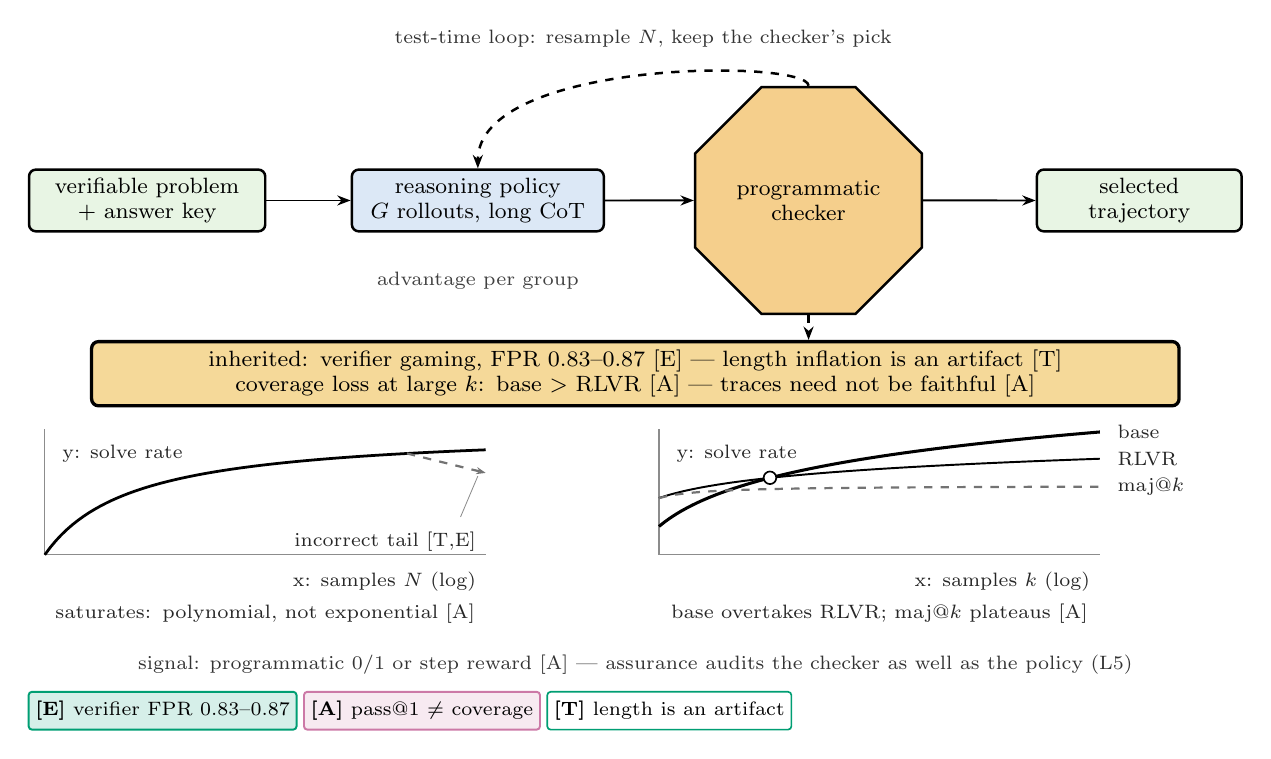
\begin{tikzpicture}[x=1mm, y=1mm]
\tikzset{
  rs/rpnote/.style={rs/gTiny, font=\fontsize{7.2}{8.6}\selectfont, text=black!85},
}
% ===== (a) chain: problem -> rollouts -> checker -> selected trajectory =====
\node[rs/gData,  minimum width=30mm] (prob) at (15,0)  {verifiable problem\\+ answer key};
\node[rs/gModel, minimum width=32mm] (roll) at (57,0)  {reasoning policy\\$G$ rollouts, long CoT};
\node[rs/gControl, minimum width=21mm] (chk) at (99,0) {programmatic\\checker};
\node[rs/gData,  minimum width=26mm] (out)  at (141,0) {selected\\trajectory};
\draw[rs/gFlow] (prob.east) -- (roll.west);
\draw[rs/gFlow] (roll.east) -- (chk.west);
\draw[rs/gFlow] (chk.east)  -- (out.west);
% test-time loop: the same checker re-ranks fresh samples; training is the tape, not this arc
\draw[rs/gFlowD] (chk.north) .. controls (99,18) and (57,18) .. (roll.north);
\node[rs/gEdgeLbl] at (78,20.5) {test-time loop: resample $N$, keep the checker's pick};
% ===== (b) inherited-failure strip (the ONE accent; hung off the checker it optimizes) =====
\node[rs/gAccent, align=center, text width=136mm, inner sep=3pt] (fail) at (77,-22)
  {inherited: verifier gaming, FPR 0.83--0.87 [E] \textemdash{} length inflation is an artifact [T]\\
   coverage loss at large $k$: base $>$ RLVR [A] \textemdash{} traces need not be faithful [A]};
\draw[rs/gFlowD] (chk.south) -- (chk.south |- fail.north);
% ===== (c) compute saturates: rational curve (algebraic tail), incorrect-tail stub =====
\begin{scope}[shift={(2,-45)}]
  \draw[black!45, line width=0.4pt] (0,0) -- (56,0);
  \draw[black!45, line width=0.4pt] (0,0) -- (0,16);
  \draw[line width=1.0pt] plot[domain=0:56, samples=80]
    (\x, {16*(\x/56)/((\x/56)+0.20)});
  % not a continuation of the fit: marks the incorrect-tail-dominant regime (dashed = regime)
  \draw[black!55, line width=0.8pt, dashed, -{Stealth[length=1.2mm]}]
    (46,12.87) -- (56,10.4);
  \node[rs/rpnote, anchor=north west] at (1,15.2) {y: solve rate};
  \node[rs/rpnote, anchor=north east] at (56,-1)  {x: samples $N$ (log)};
  \node[rs/rpnote, anchor=north east] at (56,4.2) {incorrect tail [T,E]};
  \draw[black!45, line width=0.3pt] (52.8,4.8) -- (55,10.0);
  \node[rs/rpnote, align=center, text width=58mm] at (28,-7.5)
    {saturates: polynomial, not exponential [A]};
\end{scope}
% ===== (d) pass@k vs maj@k: coverage climbs, maj plateaus, base overtakes RLVR =====
\begin{scope}[shift={(80,-45)}]
  \draw[black!45, line width=0.4pt] (0,0) -- (56,0);
  \draw[black!45, line width=0.4pt] (0,0) -- (0,16);
  % base pass@k: log-linear, still climbing at the right edge
  \draw[line width=1.1pt] plot[domain=0:56, samples=80]
    (\x, {3.6+12*ln(1+9*(\x/56))/ln(10)});
  % RLVR pass@k: starts above base, grows slowly, is overtaken
  \draw[line width=0.7pt] plot[domain=0:56, samples=80]
    (\x, {7.2+5*ln(1+9*(\x/56))/ln(10)});
  % maj@k: same pass@1 as the RLVR policy, then flat past a few hundred samples
  \draw[black!55, line width=0.8pt, dashed] plot[domain=0:56, samples=80]
    (\x, {7.2+1.6*(1-1/(1+10*(\x/56)))});
  % crossover: no rate is marked, the open dot only says where the two orders swap
  \draw[line width=0.6pt, fill=white] (14.1,9.78) circle[radius=0.8mm];
  \node[rs/rpnote, anchor=west]  at (57,15.6) {base};
  \node[rs/rpnote, anchor=west]  at (57,12.2) {RLVR};
  \node[rs/rpnote, anchor=west]  at (57,8.65) {maj@$k$};
  \node[rs/rpnote, anchor=north west] at (1,15.2) {y: solve rate};
  \node[rs/rpnote, anchor=north east] at (56,-1)  {x: samples $k$ (log)};
  \node[rs/rpnote, align=center, text width=58mm] at (28,-7.5)
    {base overtakes RLVR; maj@$k$ plateaus [A]};
\end{scope}
% ===== foot: the training signal, and what L5 audits =====
\node[rs/gFoot] (foot) at (77,-59)
  {signal: programmatic 0/1 or step reward [A] \textemdash{} assurance audits the checker as well as the policy (L5)};
% --- loss tape: one advantage per rollout group (parallel samples, one score) ---
\rsLossTape{rlvr}{roll.south}{-2.4mm}{advantage per group}
% --- evidence ribbon: segments are claims already carried above; tag = the claim's class ---
\rsRibbonBase{-3.4mm}
\rsRibbonRow{0mm}
\rsRibSeg{rsVerified}{\textbf{[E]} verifier FPR 0.83--0.87}
\rsRibSeg{rsAuthorRep}{\textbf{[A]} pass@1 $\ne$ coverage}
\rsRibSeg{rsTheory}{\textbf{[T]} length is an artifact}
\end{tikzpicture}
}
  \caption{Family card: reasoning post-training (verifier gaming as the inherited failure).}
  \label{fig:fam-reasoning}
\end{figure}

\textit{Optimizes} expected verifiable reward over a rollout group: a programmatic checker scores
sampled chains under KL/clip, keeping the autoregressive factorization and changing only the
signal. \textit{Excels at} domains with executable ground truth, where it converts latent capability
into pass@1 --- R1-Zero moves AIME 2024 from 15.6 to 77.9~\cite{id250112948}. \textit{Fails at} the
checker: fuzzed verifiers return false-positive rates of 0.832, 0.869 and 0.557 by verifier
family~\cite{id260601066}; on Qwen2.5-Math-7B/MATH-500, randomly assigned rewards still buy
21.4 pp of gain against 29.1 pp from ground truth, though Llama3 and OLMo2 do not reproduce the
gain~\cite{id250610947}; base models overtake their RLVR versions at large $k$~\cite{id250413837};
length inflation follows from the loss on incorrect answers~\cite{id250405185}; returns diminish
polynomially~\cite{id261019362}; and traces need not be
faithful~\cite{id230504388}. \textit{Complements:} typed outputs make rewards checkable
(\S\ref{sec:contracts}); assurance audits the checker as well as the policy.

\paragraph{Hierarchical code prediction (NCM-class).}
\textit{Optimizes} a coarse-to-fine factorization over levels with a residual-VQ code signal: a frozen multiscale residual VQ-VAE tokenizer
represents text as $K$ levels of discrete codes over $L$ tokens (with $\ell_k$ the number of
code positions at level $k$, $K \ll L$), and a
transformer generates each level in one parallel forward pass conditioned on the cumulative
reconstruction --- inheriting next-scale prediction from image hierarchies
\cite{kumbong2026ncm}. \textit{Excels at} short generation paths ($K \ll L$):
\evaurep{reports 21$\times$ faster decoding on LM1B at matched parameter scale and 31$\times$ on
XSum at matched ROUGE-L}, with quality at or above masked-diffusion baselines,
\evaurep{Sudoku accuracy above all evaluated baselines}, and \evaurep{$4.9\times$ lower
training-token exposure}~\cite{kumbong2026ncm}.
\textit{Fails at} tokenizer-stage semantic risk: reconstruction is near-exact per dataset (\evaurep{98.79--100\%}), but the released evaluation shows
substitutions of named entities or numerals --- a \evaurep{99.79\%-reconstruction summarisation case}
does not certify meaning-level fidelity --- and the tokenizer fixes
what downstream checks can distinguish. Math/data/correctness goals shift the exact-recovery
requirement, and the authors' conditioning-corruption training buys code-error robustness inside
the representation, not at the contract ([A]-class). \textit{Complements:} output contracts must define token-exactness vs.\
meaning-equivalence boundaries; acceptance machinery resumes.

\begin{figure}[t]\centering
  \resizebox{\linewidth}{!}{% fig:fam-ncm — NCM-class mechanism sketch (figure-design-standard gate-1 spec, v6)
% TAKEAWAY: staged-tokenizer generation relocates the envelope to the code hierarchy
% (token-exact NOT meaning-equivalent; codebook-error compounding is contested).
% Grammar: accent link SOLID (ledger-[E]-anchored); compounding link DASHED (contested,
% no production guard). Glosses live in ONE full-width note box (no seam, no overhang),
% anchored by two thin leaders. Heights normalised (10mm band); 8mm chain gaps.
% CAPTION NOTE: amber = tokenizer-stage semantic risk [E]; dashed = contested compounding;
% 4.9x-token claim lives in section text.
% RIBBON (P1 pilot): evidence strip below the card — one segment per claim already carried
% by this card or its section paragraph; tags use the reserved rs* evidence colours with
% letter badges; theory/vendor classes are OUTLINE-only (rsTheory/rsVendor) so they never
% read as the gray null class; dashed border = contested (same grammar as the dashed edge).
% LOSS TAPE (P3): three rows of parallel terms = the per-level prediction structure; lives
% in the free band between the chain and the two risk boxes (no edge crosses it).
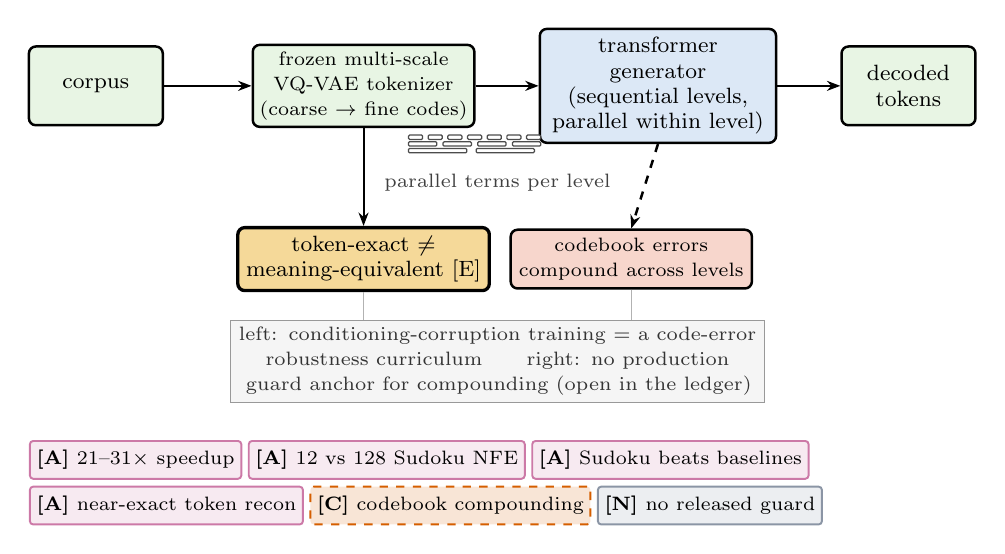
\begin{tikzpicture}[x=1mm, y=1mm]
  \node[rs/gData,  minimum width=17mm, minimum height=10mm] (corpus) at (0,0)   {corpus};
  % tokenizer label is text-saturated (27pt of ink in a 10mm box, 0.6mm margins): the
  % record-rules mark cannot clear it, so this box drops the interior mark (style keeps
  % rules for every store with headroom); role stays legible from the label itself.
  \node[rs/gStore, path picture=, minimum width=26mm, minimum height=10mm] (tok)    at (34,0)  {frozen multi-scale\\VQ-VAE tokenizer\\(coarse $\to$ fine codes)};
  \node[rs/gModel, minimum width=30mm, minimum height=12mm, right=8mm of tok] (gen) {transformer\\generator\\(sequential levels,\\parallel within level)};
  \node[rs/gData,  minimum width=17mm, minimum height=10mm, right=8mm of gen] (out) {decoded\\tokens};
  \node[rs/gAccent, align=center, minimum width=26mm] (accent)   at (34,-22) {token-exact $\ne$\\meaning-equivalent [E]};
  \node[rs/gRisk,   align=center, minimum width=26mm] (compound) at (68,-22) {codebook errors\\compound across levels};
  \draw[rs/gFlow]  (corpus) -- (tok);
  \draw[rs/gFlow]  (tok) -- (gen);
  \draw[rs/gFlow]  (gen) -- (out);
  \draw[rs/gFlow]  (tok.south) -- (accent.north);
  \draw[rs/gFlowD] (gen.south) -- (compound.north);
  % --- single full-width note band, leader-anchored to both risk items
  \node[rs/gFoot, align=center, draw=black!40, fill=black!4, inner sep=2.5pt, text width=66mm]
    (gloss) at (51,-35) {left: conditioning-corruption training = a code-error robustness curriculum~~~~~
    right: no production guard anchor for compounding (open in the ledger)};
  \draw[black!30, line width=0.4pt] (accent.south) -- (gloss.north -| accent.south);
  \draw[black!30, line width=0.4pt] (compound.south) -- (gloss.north -| compound.south);
  % --- loss tape (P3): levels are sequential, terms within a level are parallel.
  % Sits in the free band between the chain and the two risk boxes; the vertical edges at
  % x=34 (tokenizer) and x=68 (compounding) stay outside the 30mm label.
  \coordinate (ntape) at (51,-8.5);
  \rsLossTape{ncm}{ntape}{0mm}{parallel terms per level}
  % --- evidence ribbon (P1): one segment per claim already in the card / its section text.
  % Two rows because six full labels in one row exceed the card's natural width and would
  % down-scale the whole picture (font floor); each row stays inside the card's bbox width.
  \rsRibbonAt{-8.5}{-47.5}
  \rsRibSeg{rsAuthorRep}{\textbf{[A]} 21--31$\times$ speedup}
  \rsRibSeg{rsAuthorRep}{\textbf{[A]} 12 vs 128 Sudoku NFE}
  \rsRibSeg{rsAuthorRep}{\textbf{[A]} Sudoku beats baselines}
  \rsRibbonAt{-8.5}{-53.3}
  \rsRibSeg{rsAuthorRep}{\textbf{[A]} near-exact token recon}
  \rsRibSeg[dashed]{rsContested}{\textbf{[C]} codebook compounding}
  \rsRibSeg{rsNoClaim}{\textbf{[N]} no released guard}
\end{tikzpicture}
}
  \caption{Family card: hierarchical code prediction (NCM-class). Accent = the tokenizer-stage semantic-risk boundary; dashed = contested/undocumented wiring (codebook compounding). Speed, NFE and Sudoku evidence is highlighted on the ribbon. Ribbon segments carry the dominant class ([T]/[E]/[A]/[V]); the full alphabet is \cref{tab:evidence-classes}. Colour key: teal = [E] independently evaluated, purple = [A] author-reported, teal outline = [T] theory-under-assumptions, purple outline = [V] vendor-reported, vermillion = [C] contradicted (anchor named), gray = [N] not claimable; all dashed outlines = contradicted (global dashed grammar). The frozen tokenizer is drawn as a store: a fixed codebook consulted at generation, not a component trained in this card.}
  \label{fig:fam-ncm}
\end{figure}

A schedule is a factorization choice, not an architecture, and the objective families above
instantiate three of them (\cref{fig:schedule-atlas}). Autoregressive generation is the chain
rule: one commitment per token, none revisable. Iterative denoising revisits every position on
every pass, so revision is free but nothing is settled until the last pass. Coarse-to-fine
hierarchies commit one level at a time and stay revisable until the next level resolves them,
at $K \ll L$ sequential steps. What differs across the three is how many sequential decisions
an output contract must accept and whether any of them can be taken back --- the quantity a
contract inspects at acceptance time (\cref{sec:contracts}).

\begin{figure}[t]\centering
  \resizebox{\linewidth}{!}{% figures/f_schedule_atlas.tex — G1: generation-schedule atlas (three factorizations, one picture).
% TAKEAWAY: the three families differ mainly in HOW MANY sequential decisions they make and
% whether a decision can be revised — AR commits per token, masked diffusion refines all
% positions every pass, NCM-class commits K coarse-to-fine levels (K << L).
% Grammar: style_v2_tokens.tex roles only (rs/gData payload green, rs/gModel mechanism).
%   No accent colour (this figure defends no single ledger item). Dashed survives ONLY as the
%   diagnostic preview port (off the generation path, labelled); no contested [C] wiring is drawn.
% Labels >= 7.5pt; math rides 8.2pt (CMSY measures ~0.92x); NO math sub/superscripts — level
%   indices and z-tap indices ride as TEXT digits, or they would publish below the 7pt floor.
% The only quantitative claim is K << L; step counts are symbolic (Lx1, TxL, Kxl_k), no clock.
\providecommand{\atlasll}{{\fontsize{8.2}{10}\selectfont $K \ll L$}}
\providecommand{\atlasdots}{{\fontsize{8.2}{10}\selectfont $\cdots$}}
\providecommand{\atlasT}{{\fontsize{8.2}{10}\selectfont $T$}}
% level labels ride 8.2pt math and a TEXT digit: a math subscript would publish at 5.6pt
\providecommand{\atlasell}[1]{{\fontsize{8.2}{10}\selectfont $\ell$}#1}
% z tap labels: 8.2pt glyph + TEXT index, same sub-floor reason
\providecommand{\atlasz}{{\fontsize{8.2}{10}\selectfont $z$}}
\providecommand{\atlaszof}[1]{{\fontsize{8.2}{10}\selectfont $z$}(#1)}
\begin{tikzpicture}[x=1mm, y=1mm]
\tikzset{
  rsa/lane/.style={anchor=west, font=\fontsize{8.2}{9.8}\selectfont\bfseries, text=black},
  rsa/cell/.style={draw=black!70, line width=0.6pt, fill=rsGreenPale, align=center,
                   font=\fontsize{7.5}{9.0}\selectfont, inner sep=0.6pt, minimum height=5mm},
  rsa/note/.style={anchor=west, font=\fontsize{7.5}{9.0}\selectfont, text=black!85},
  rsa/cost/.style={anchor=west, font=\fontsize{7.5}{9.0}\selectfont, text=black!70},
}
% ============ lane 1: autoregressive — L sequential, non-revisable commitments ============
\node[rsa/lane] at (0,0) {AR};
\node[rsa/note] at (0,-4.4) {next-token chain};
\node[rsa/cost] at (0,-8.3) {{\fontsize{8.2}{10}\selectfont $L\times1$} --- revision: none};
\foreach \i/\lab in {0/the, 1/f, 2/ul, 3/l} {
  \node[rsa/cell, minimum width=7mm] at (44+\i*9,0) {\lab};
}
\foreach \i in {4,...,8} {
  \node[rsa/cell, minimum width=7mm, fill=white] at (44+\i*9,0) {};
}
\node[rsa/note] at (121.5,-1.6) {\atlasdots};
% per-token commitment arrows: each token is committed when emitted, with no revision path back
\foreach \i in {0,...,8} {
  \draw[-{Stealth[length=1.4mm]}, line width=0.6pt, draw=black!75]
    (44+\i*9,-2.7) -- (44+\i*9,-7.3);
}
\draw[line width=0.6pt, draw=black!45] (40.5,-7.6) -- (119.5,-7.6);
\node[rsa/note] at (44,-11.4) {L sequential steps; each token commits (non-revisable)};

% ============ lane 2: masked diffusion — T passes over ALL L positions ============
\node[rsa/lane] at (0,-22) {masked diffusion};
\node[rsa/note, text width=31mm] at (0,-26.4) {iterative denoising, all positions revisited};
\node[rsa/cost] at (0,-33.4) {{\fontsize{8.2}{10}\selectfont $T\times L$} --- revision: all};
% three snapshots (t=T / one intermediate / t=0). The intermediate reveal is SCATTERED, not a
% prefix: a prefix is the AR picture this lane must not borrow. Settled cells are darker.
\foreach \c in {0,...,8} {
  \node[rsa/cell, minimum width=7mm, fill opacity=0.12, text=black!80]
    at (44+\c*8.4,-22) {?};
}
\foreach \c/\t in {0/the, 4/re, 7/le} {
  \node[rsa/cell, minimum width=7mm, fill opacity=0.85, text=black!85]
    at (44+\c*8.4,-30) {\t};
}
\foreach \c in {1,2,3,5,6,8} {
  \node[rsa/cell, minimum width=7mm, fill opacity=0.30, text=black!80]
    at (44+\c*8.4,-30) {?};
}
\foreach \c/\t in {0/the, 1/f, 2/ul, 3/l, 4/re, 5/li, 6/ab, 7/le, 8/.} {
  \node[rsa/cell, minimum width=7mm, fill opacity=0.95, text=black!85]
    at (44+\c*8.4,-38) {\t};
}
% re-mask: a settled cell can return to `?` between passes — self-loop above cell 4, labelled.
\draw[-{Stealth[length=1.1mm]}, line width=0.75pt, draw=black!65]
  (76.3,-27.7) .. controls (75.4,-25.3) and (79.8,-25.3) .. (78.9,-27.7);
\node[rsa/note] at (80.2,-26.0) {re-mask};
% the pass axis: one arrow for T, not per-cell arrows
\draw[-{Stealth[length=1.6mm]}, line width=0.7pt, draw=black!65] (118,-19.5) -- (118,-40.5);
\node[rsa/note] at (120,-30) {\atlasT{} passes};
\node[rsa/note] at (44,-44.8) {T denoise passes over ALL L positions; any position re-masked};

% ============ lane 3: NCM-class — K sequential levels, parallel within a level ============
\node[rsa/lane] at (0,-55) {NCM-class};
\node[rsa/note, align=left] at (0,-59.4)
  {corpus / tokenizer:\\K code levels};
\node[rsa/cost, align=left] at (0,-65.6)
  {{\fontsize{8.2}{10}\selectfont $K\times$}\atlasell{k}\\{}revision: residual};
% same-span level rows: every level spans x=44..108 while cells shrink as l_k grows and fill
% darkens with detail — the SAME sequence at rising resolution, not a row that appends rightward.
\foreach \r/\n/\idx/\op in {0/2/1/0.30, 1/4/2/0.50, 2/7/3/0.72, 3/10/4/0.95} {
  \pgfmathsetmacro{\cw}{(64-(\n-1)*0.7)/\n}
  \pgfmathsetmacro{\nm}{\n-1}
  \node[rsa/note, anchor=east] at (38,-55-\r*6) {\atlasell{\idx}};
  \foreach \c in {0,...,\nm} {
    \pgfmathsetmacro{\cx}{44+\c*(\cw+0.7)+\cw/2}
    \node[rsa/cell, minimum width=\cw mm, fill opacity=\op, text=black!80]
      at (\cx,-55-\r*6) {};
  }
  % one hand-off per level (parallel within the level): its codes join the cumulative z(k)
  \draw[-{Stealth[length=1.4mm]}, line width=0.7pt, draw=black!70]
    (108,-55-\r*6) -- (117.6,-55-\r*6);
  \fill[black!70] (118,-55-\r*6) circle (0.55);
  \pgfmathtruncatemacro{\kp}{\r+1}
  \node[rsa/note, anchor=south east] at (117.4,-54.1-\r*6) {\atlaszof{\kp}};
  % diagnostic preview port (dashed, off the cost path, above the tap so it never grazes the
  % decode box); omitted at level K, whose decode is real
  \ifnum\r<3
    \draw[line width=0.6pt, draw=black!55, dashed] (118,-55-\r*6) -- (119.7,-53.9-\r*6);
    \draw[line width=0.55pt, draw=black!55, fill=white] (119.9,-53.7-\r*6) circle (0.42);
  \fi
}
% conditioning spine: thin left rail from the corpus/tokenizer past every level, one tick per level
\draw[line width=0.6pt, draw=black!60] (41.5,-51.4) -- (41.5,-73);
\fill[black!60] (41.5,-51.4) circle (0.45);
\foreach \r in {0,...,3} {
  \draw[-{Stealth[length=1.1mm]}, line width=0.6pt, draw=black!60]
    (41.5,-55-\r*6) -- (43.7,-55-\r*6);
}
\node[rsa/note] at (0,-51.2) {conditioned on \atlasz(k-1)};
% one decode, after the last level: the acceptance surface, not a per-level step
\draw[line width=0.6pt, draw=black!60] (118,-55) -- (118,-73);
\node[rs/gModel, anchor=west, minimum width=22mm, minimum height=11mm, text width=19mm,
      inner xsep=2pt, inner ysep=2pt, font=\fontsize{7.5}{9.0}\selectfont] (dec)
  at (120,-73) {decode once\\acceptance\\surface};
\draw[-{Stealth[length=1.4mm]}, line width=0.7pt, draw=black!70] (118,-73) -- (dec.west);
\node[rsa/note] at (121.2,-53.8) {previews};
\node[rsa/note] at (44,-81.4) {K steps of sequential levels, parallel within level; \atlasll};
% preview ports are diagnostic; the sole generation-path decode is the box above
\end{tikzpicture}
}
  \caption{ Generation-schedule atlas: the three factorizations differ in how many sequential decisions they make and whether a decision can be revised. Lanes are in Table 1 order, not cost-ranked: left-to-right chain rule ($L\times1$: one commitment per token, never revised), iterative sequence denoising ($T\times L$: every position revisited each pass, so any position can be re-masked), and the coarse-to-fine code hierarchy ($K$ sequential levels with $\ell_k$ code positions at level $k$, parallel within a level; every level spans the same token sequence at rising resolution, it does not append). Each level is fed by the conditioning spine (conditioned on $z(k{-}1)$) and hands its codes to a cumulative reconstruction $z(k)$; a single decode follows the last level and is the acceptance surface. Dashed ports are diagnostic per-level previews off the $K$-step path. The only quantitative claim is $K\ll L$; no wall-clock numbers are drawn.}
  \label{fig:schedule-atlas}
\end{figure}


\paragraph{What the cards jointly establish.}
\looseness=-1
No family wins across currencies: likelihood, fidelity, calibration and semantic correctness
are different objectives, so a stack that mixes families (L1) with contracts (L4) and
assurance (L5) is the actual engineering answer, and Section~\ref{sec:selection} formalizes
the choice.


\section{Layer 2 --- Representations and What They Guarantee}\label{sec:representations}
% ===== L2 draft: Layer 2 -- Representations and What They Guarantee (first written pass, 2026-10-17)
% \input directly under \section{Layer 2 ...}\label{sec:representations}; starts at subsection level.
% p2 placeholders beyond the pre-cleared list: id260723531 (JEPA Paradox in Language; openpins
% CONFIRMED 2026-10-17, evidence _scan/openpins_evidence/html_2607.23531.html) and id230108243
% (I-JEPA, SLR pin). Both verified in-repo; add to the conversion table when merging.

\subsection{Representation as the interface between objective and system}
\label{sec:l2-interface}

The first layer decides what a model is trained to be (\cref{sec:objectives}), and the second
decides what the input becomes; a \emph{representation} is the interface between the two. It
fixes the objects the system computes over, and with them the assumptions that every later layer
(inference architecture, output contract, assurance) inherits. Three families recur across the
stack instances of \cref{sec:stack}. (i)~\emph{Token embeddings}: a discrete sequence of subword
units, represented as learned vectors. This is the dominant interface of language systems, and
it embeds a modelling decision that is easy to overlook. \evindep{Tokenization is more than
compression: comparative studies find that tokenization choices impose inductive biases of their
own, with downstream consequences that compression ratio does not predict \cite{id240218376}.}
Byte-level and multiscale byte-sequence designs (the ByT5/MEGABYTE class) relax or remove the
tokenizer at the cost of longer effective sequences, though multiscale byte transformers were
designed to amortize that cost \cite{id230507185}.
(ii)~\emph{Encoder and joint-embedding latents}: a continuous vector space trained by prediction
or agreement, spanning the JEPA family and the embedding models that retrieval consumes.
(iii)~\emph{Symbolic or structured state}: retrieved spans, typed records, explicit task state,
representations on which deterministic checks are possible by construction. The rest of this
section asks what each family guarantees, and what it hands to the layers that follow.

\subsection{Joint-embedding latent prediction and the language-{JEPA} paradox}
\label{sec:l2-jepa}

Joint-embedding predictive training predicts target \emph{representations} rather than raw
inputs: a context encoder observes a masked view, an exponential-moving-average (EMA) target
encoder embeds the unmasked signal, and a predictor is trained to match the target latent. What
the objective encourages is a representation in which masked targets are predictable from the
visible context, one biased toward structure from the outset rather than toward surface
reconstruction. The family produced strong visual representations (I-JEPA \cite{id230108243})
and motivates the hope that such learning yields a world model rather than a surface generator.
Its language case tests our honesty most directly, so we state it as a conditional candidate
rather than a verdict.

\evtheory{Squared-error latent prediction is well posed only when the target representation is
conditionally concentrated---when, given the context and the target location, the target
representation lies near a single meaningful point. Otherwise the optimal predictor degenerates
to a conditional mean: a centroid over incompatible alternatives.} Masked text need not satisfy
this condition: the same context can admit several valid continuations whose embeddings occupy
distinct directions. \evindep{In matched I-JEPA/T-JEPA experiments, mutual-information
saturation and elevated conditional target variance precede train--validation divergence,
effective-rank degeneration, cosine collapse, and poor downstream transfer; the pattern
replicates across five independent data seeds, and downstream probes (IMDB and SNLI
classification; MTEB retrieval, FEVER and MSMARCO) fail to transfer \cite{id260723531}.} The
study is explicit that this does not refute predictive learning for language; it identifies a
missing inductive bias, namely the preservation of multiple plausible completions instead of
compressing them into one latent point. The same analysis notes that marginal variance
regularizers constrain only the marginal distribution, so they do not by themselves guarantee
predictable conditionals \cite{id260723531}.

Identifiability theory for latent world models (the conditions under which a learned latent
provably corresponds to the structure that generated the data) is recent and explicitly
conditional. \evtheory{Results on when JEPA-style training learns an identifiable world model,
and on the identifiability of controlled world models, hold under stated assumptions about data
and training; extensions relax the Gaussianity restriction without making identifiability
unconditional \cite{klindt2026lejepa,identifiability2026,id260612471}.} We take a standing
discipline from this cluster: prediction quality and world-model quality are separate
properties. Low squared error on held-out targets can coexist with degenerate representation
geometry, and whatever structure a representation recovers is recovered only because the stated
assumptions hold; the objective does not deliver it by default.

\subsection{World models: prediction quality is not decision quality}
\label{sec:l2-worldmodels}

When Layer~2 hands a world model to a planner, the reliability question changes register. The
world-models survey we cite as our anchor treats objectives and representations together
\cite{id251016732}; its scope is robotics-oriented, and we borrow from it only the interface
claim we need here: serving a model to a decision procedure differs from evaluating it as a
predictor. \evsynth{Prediction metrics and decision utility are different currencies: a model can
minimize average rollout error and still be a poor or exploitable basis for planning, because
decisions consume predictions through an optimizer whose failure modes---compounding error,
exploitation of model error, objective mismatch---need not appear in any prediction loss.}
Planning needs more than prediction: it needs predictions that are reliable exactly where the
decision is sensitive, which is a statement about the task and the policy (L0, L3--L4), as
\cref{sec:selection} sets out. The identifiability results above also govern
expectations here: where their assumptions hold, ``the representation is a world model'' has
content; where they fail, the same phrase is an aspiration. Unqualified world-model
claims are unsupported without those assumptions; since they cannot be evidenced, they have to
be gated, which makes them a matter for the assurance layer (\cref{sec:assurance}).

\subsection{What each representation choice hands to the output and assurance layers}
\label{sec:l2-handoff}

Representation choices propagate downstream: each family of \cref{sec:l2-interface} hands Layer~4
(\cref{sec:contracts}) and Layer~5 (\cref{sec:assurance}) different raw material.

\emph{Token embeddings.} The system can emit a distribution over a discrete alphabet, so output
contracts built on checking discrete structure---schemas, grammars
\cite{jsonschemabench2025,xgrammar2024}---have something to verify; what they verify is structure;
the boundary to truth is Layer~4's central statement (\cref{sec:contracts}). One
deployment-level asymmetry matters for reliability: in API-served models the tokenizer is fixed
by the serving stack, so tokenization-induced biases are inherited rather than chosen and cannot
be repaired by output constraints alone. One recent variant replaces the subword tokenizer
itself with a learned multiscale code hierarchy (NCM-class \cite{kumbong2026ncm}):
\evaurep{surface reconstruction is 98.79--100\% across the released datasets (99.79\% on XSum),
yet the authors observe substitutions of named entities and numerals and errors in diacritics and
usernames at the tokenizer stage}. \evsynth{What such a representation hands Layer~4 is
a boundary to define --- token exactness vs.\ meaning equivalence --- rather than a fidelity
guarantee to inherit (\cref{sec:contracts}).}

\emph{Joint-embedding latents.} Similarity geometry and probability semantics answer different
questions: a cosine score has no declared meaning, so no threshold policy can consume it.
\evtheory{Threshold policies---abstention, escalation, cascades---need a scalar risk
estimate with a declared meaning, which a raw embedding does not provide; obtaining one requires
adding a calibration or conformal layer together with its own assumptions (exchangeability for
conformal procedures; alignment conditions for provable abstention)
\cite{id240501563,id260704430}.} The calibration and uncertainty surveys map what
confidence estimates do and do not carry for LLM systems \cite{id231108298,id250315850},
and abstention designs (surveyed in \cite{id240718418}) are the constructive response. Output
contracts that emit typed decision probabilities as first-class outputs
\cite{rauk2026jevbenchmark} occupy exactly this design point: they make the decision probability,
not a similarity score, the object that a threshold policy consumes.

\emph{Byte-level input.} Removing the tokenizer trades a class of tokenizer-induced failure modes
for sequence length; attention cost grows super-linearly in length \cite{vaswani2017attention},
so the context budget that finer granularity spends is unavailable to retrieval and verification
machinery unless multiscale designs buy it back \cite{id230507185}. The pattern generalizes:
representations do not determine reliability, but they determine which reliability mechanisms are
available downstream, and \cref{sec:selection} follows that thread.

\subsection{What Layer 2 does not guarantee}
\label{sec:l2-limits}

\evtheory{Identifiability is never unconditional: the results cited in this section hold under
stated assumptions about data and training, and outside them nothing follows.} Representation and
semantics are distinct: a latent can be stable and low-loss yet underdetermined with
respect to the meaning a decision needs. The language case remains open in both directions:
\evindep{%
deterministic squared-error latent prediction fails under matched protocols on text
\cite{id260723531}, while the same authors leave predictive representation learning for
language explicitly unrefuted.} We therefore record \emph{stable language-JEPA as contested}: a
candidate the field has neither established nor settled, and an honest-null entry in the ledger
of \cref{sec:protocol}; at matched evidence standards, no language representation recipe in our
ledger carries the evidence its image- and video-modality ancestors do~\textsf{[N]} (scoped to the
searched literature, cutoff 2026-10-17).

\FloatBarrier

\noindent The mechanism is sketched in \cref{fig:layer2-reps}.
\begin{figure}[t]\centering
  \resizebox{\linewidth}{!}{% figures/f_layer2_reps.tex — L2 mechanism sketch: representation families, forked at the
% tokenizer, and the checkability each family hands downstream (v4 2026-10-19).
% Grammar: figures/style_v2_tokens.tex (v8 token grammar). Roles: payload = rs/gData;
%   encoders / predictors / learned spaces = rs/gModel; the serving tokenizer = rs/gInfra;
%   yellow accent = the item the evidence ledger defends for L2. Solid = documented mechanism;
%   dashed = alternative / claim-to-defend (caption must cite).
% Change from v3: the three right-hand "space" boxes are gone; the right edge is one handoff
%   rule (x=109) whose entries are the paper's own affordance claims, so the foot's three
%   clauses now sit on the marks they qualify. The byte lane is a fork off lane (i) at the
%   input (tokenizer vs no tokenizer), not a third lane. Lane (iii) — the symbolic/structured
%   state family the section names ("checks possible by construction") — is drawn.
% label: fig:layer2-reps   (figure env + \label to be wired in main.tex, sec:representations)
%
% CAPTION NOTE — items the paper must defend (state these in the caption):
%   1. yellow [T]: identifiability trio klindt2026lejepa + identifiability2026 + id260612471
%      (2605.26379 / 2607.22430 / 2606.12471) — a learned latent corresponds to the generating
%      structure only under the stated data/training assumptions; assumption-bound, not an [E]
%      operational guarantee; no anchor bridges identifiability to decision quality [GAP];
%   2. prediction is not planning: low latent-prediction error coexists with degenerate geometry
%      (2607.23531 [E], cosine collapse + rank degeneration, five seeds); prediction metrics are
%      not decision utility [S];
%   3. tokenization: effects are [S/E] (2402.18376) — biases do not follow from compression
%      ratio; in API-served models the tokenizer is fixed by the serving stack (inherited);
%   4. byte fork (dashed) = tokenizer-free alternative, MEGABYTE class 2305.07185: trades
%      tokenizer failure modes for longer effective sequences; tagged [S] in the figure (design
%      evidence, author-reported in the source, no independent head-to-head in our set). The
%      undefined "[F]" that v3 printed here is retired (audit H10, figure side);
%   5. handoff downward: contracts (L4) can check discrete structure, not truth; embedding
%      similarity is not probability semantics — a scalar risk estimate needs calibration /
%      conformal machinery with its own assumptions (2405.01563, 2607.04430).
% Fonts >= 7.5pt; math glyphs measure ~0.92x nominal (CMSY/CMR quirk) so symbols use 8.2pt.
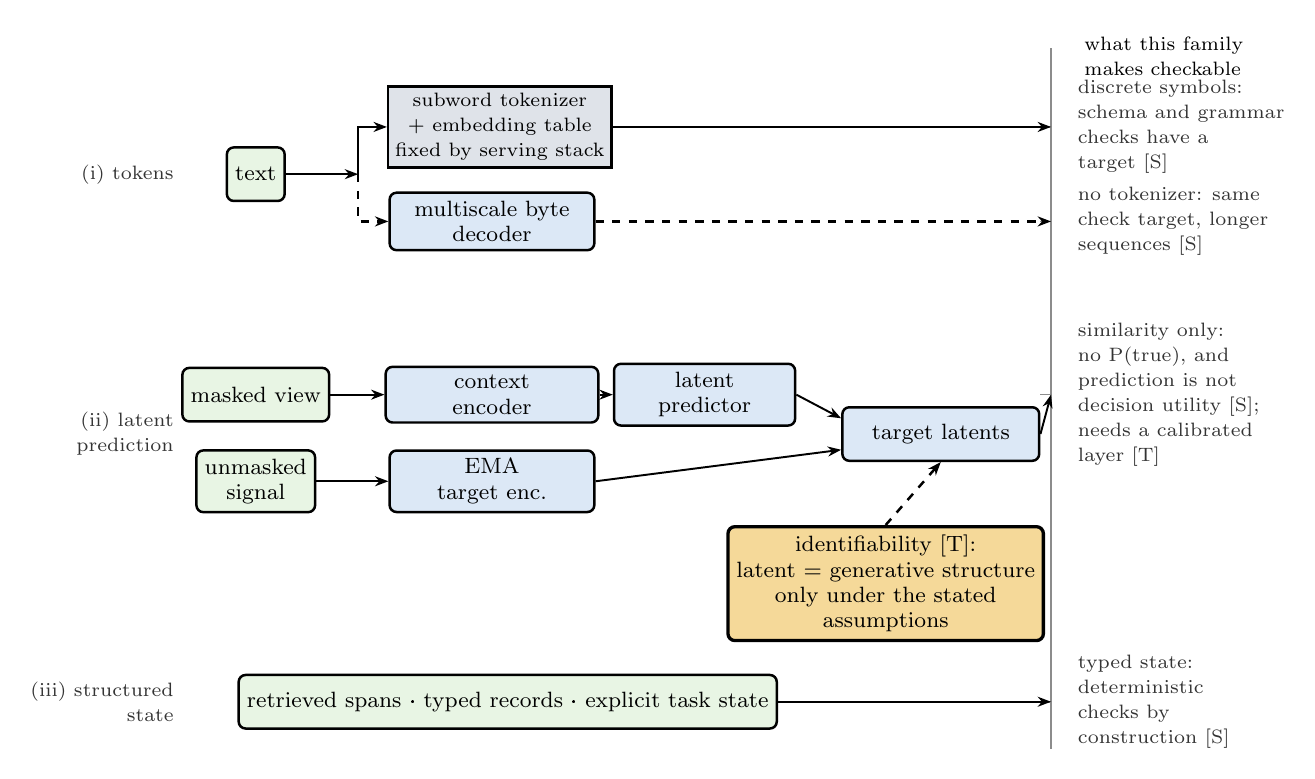
\begin{tikzpicture}[x=1mm,y=1mm]
\tikzset{
  rs/l2note/.style={rs/gEdgeLbl, anchor=east, align=right},
  rs/l2entry/.style={rs/gEdgeLbl, anchor=west, align=left, text=black!80},
  rs/l2head/.style={rs/gLegend, anchor=west, align=left},
}
% ===== right-edge handoff rule: what each family makes checkable =====
\draw[black!45, line width=0.6pt] (109,20) -- (109,-69);
\foreach \yy in {10,-2,-24,-63} { \draw[black!45, line width=0.6pt] (107.6,\yy) -- (109,\yy); }
\node[rs/l2head] at (112,19) {what this family\\makes checkable};
% ===== lane (i): token embeddings, forked at the input =====
\node[rs/gData] (txt) at (8,4) {text};
\node[rs/gInfra, minimum width=27mm] (tokm) at (39,10) {subword tokenizer\\+ embedding table\\{\fontsize{7.5}{9}\selectfont fixed by serving stack}};
\node[rs/gModel, minimum width=26mm] (bytm) at (38,-2) {multiscale byte\\decoder};
\coordinate (fork) at (21,4);
% ===== lane (ii): joint-embedding latent prediction (two rows) =====
\node[rs/gData] (ctx) at (8,-24) {masked view};
\node[rs/gModel, minimum width=27mm] (cenc) at (38,-24) {context\\encoder};
\node[rs/gModel, minimum width=23mm] (pred) at (65,-24) {latent\\predictor};
\node[rs/gModel, minimum width=25mm] (space) at (95,-29) {target latents};
\node[rs/gData] (tgt) at (8,-35) {unmasked\\signal};
\node[rs/gModel, minimum width=26mm] (tenc) at (38,-35) {EMA\\target enc.};
% ===== yellow claim (ledger-defended item): identifiability =====
\node[rs/gAccent, minimum width=36mm] (ident) at (88,-48) {identifiability [T]:\\latent {\fontsize{8.2}{10}\selectfont$=$} generative structure\\only under the stated\\assumptions};
% ===== lane (iii): symbolic / structured state =====
\node[rs/gData, minimum width=56mm] (sym) at (40,-63) {retrieved spans \textperiodcentered{} typed records \textperiodcentered{} explicit task state};
% ===== lane captions =====
\node[rs/l2note] at (-2,4)   {(i) tokens};
\node[rs/l2note] at (-2,-29) {(ii) latent\\prediction};
\node[rs/l2note] at (-2,-63) {(iii) structured\\state};
% ===== edges =====
\draw[rs/gFlow]  (txt.east) -- (fork);
\draw[rs/gFlow]  (fork) |- (tokm.west);
\draw[rs/gFlowD] (fork) |- (bytm.west);
\draw[rs/gFlow]  (tokm.east) -- (109,10);
\draw[rs/gFlowD] (bytm.east) -- (109,-2);
\draw[rs/gFlow]  (ctx.east) -- (cenc.west);
\draw[rs/gFlow]  (cenc.east) -- (pred.west);
\draw[rs/gFlow]  (pred.east) -- ([yshift=2mm]space.west);
\draw[rs/gFlow]  (tgt.east) -- (tenc.west);
\draw[rs/gFlow]  (tenc.east) -- ([yshift=-2mm]space.west);
\draw[rs/gFlow]  (space.east) -- (109,-24);
\draw[rs/gFlow]  (sym.east) -- (109,-63);
\draw[rs/gFlowD] (ident.north) -- (space.south);
% ===== claims sited on the marks (no foot) =====
\node[rs/l2entry] at (112,10) {discrete symbols:\\schema and grammar\\checks have a\\target [S]};
\node[rs/l2entry] at (112,-2) {no tokenizer: same\\check target, longer\\sequences [S]};
\node[rs/l2entry] at (112,-24) {similarity only:\\no P(true), and\\prediction is not\\decision utility [S];\\needs a calibrated\\layer [T]};
\node[rs/l2entry] at (112,-63) {typed state:\\deterministic\\checks by\\construction [S]};
\end{tikzpicture}
}
  \caption{ Layer 2 schematic: three representation families and what each hands the layers above. Tokens are discrete symbols, so schema and grammar checks have a target; the tokenizer-free byte fork keeps that target and pays in sequence length [J]; joint-embedding latents carry similarity only --- no $P(\text{true})$ and no decision utility --- so a scalar risk estimate needs a calibration layer with its own assumptions [T]; symbolic or structured state supports deterministic checks by construction. Yellow: identifiability [T], the latent equals generative structure only under the stated assumptions, with no anchor in our set bridging it to decision quality [GAP]. In API-served models the tokenizer is fixed by the serving stack [S].}
  \label{fig:layer2-reps}
\end{figure}



\section{Layer 3 --- Inference Architectures}\label{sec:architectures}
% Layer 3 — Inference Architectures (draft pass, 2026-10-17).
% Insertion point: \section{Layer 3 --- Inference Architectures}\label{sec:architectures} in main.tex.
% Cite policy: bib keys where they exist; otherwise placeholder keys of the form p2[<verified arXiv ID>].

\subsection{Generalists, Specialists, and Hybrid Pipelines}
\label{sec:l3-mix}

Layer~3 covers the choices that govern how a trained model is \emph{used}: at what granularity, with what conditional computation, and with which external calls. The first choice is granularity. A generalist is asked to produce everything at once --- answer, format, and whatever confidence the response needs; a specialist commits to narrower outputs that a downstream system can verify mechanically: boxes, discrete labels, bounded scores. That verifiability is the argument for the specialist architecture, and also the one most often asserted rather than measured end to end. \evvendor{Interfaze positions an orchestrated set of task-specific small models against general-purpose incumbents \cite{interfaze2026}}; the claim lives at component level, and \cref{fig:case-hybrid} reconstructs one such pipeline from vendor descriptions chiefly so that the edges the vendor leaves undocumented --- monitors, validators, escalation --- stay visible in our account. The hybrid pays for composition: every added component brings its own error distribution, and the pipeline's end-to-end reliability depends on how those errors propagate, not on the best component's headline number. We therefore treat hybrid pipelines as stack instances with their own failure envelopes rather than as upgraded single models.

\subsection{Mixture-of-Experts: Routing Inside the Model}
\label{sec:l3-moe}

Mixture-of-Experts is conditional computation inside the model: capacity scales with parameter count while cost scales with activated experts, and the router becomes a learned, partially inspectable dispatch policy \cite{id240706204}. Our selection framework needs the intra-model and system-level split more sharply than the survey literature draws it, so we keep two routing loci strictly apart: \emph{intra-model} routing decides which experts fire for a token and is an architecture property; \emph{system-level} routing decides which model or cascade tier receives a request (\cref{sec:l3-routing}) and is an orchestration policy. On reliability, MoE-RBench is the benchmark evidence we anchor: \evindep{Across safety and hallucination, adversarial resilience, and out-of-distribution robustness, sparse MoE can be made more reliable than dense models of its class, but robustness is sensitive to basic training settings and hyperparameters \cite{id240611353}}. Reliability here is a tunable, configuration-dependent property. Compression follows the same logic: \evindep{structured expert pruning preserves in-domain utility at moderate ratios, whereas hallucination risk rises at extreme pruning and both utility and factual reliability degrade quickly out of domain \cite{id260701444}}; at deployment time compression is a reliability decision as much as a memory one.

\subsection{Routing and Cascades: Cost--Quality Allocation as an Architectural Lever}
\label{sec:l3-routing}

Above the model, allocation happens per query. FrugalGPT established the cascade pattern (chains of increasingly capable models whose cheaper members are trusted only when their scored responses clear a cutoff), reallocating spend toward the queries that need it \cite{frugalgpt2023}. The architectural weak point is the dispatch signal: cascades greedily select the lightest model from confidence scores, but deep models are systematically overconfident and confidence distributions differ across models and languages, so the C3 system \cite{id240215991} interposes a per-member calibration stage before escalation. SATER unifies pre-generation routing with cascade-style escalation under a token-efficiency objective, targeting the accuracy--latency split between the two families \cite{id251005164}. Routing also extends beyond a fixed pool: UniRoute routes to previously unseen models by representing each candidate through its predictions, with excess-risk bounds relating the learned rule to a theoretical optimum \cite{id250208773}. The evidence base remains fragmented. The characterization survey of routing and hierarchical inference is efficiency-scoped and notes the absence of a unified evaluation across methods \cite{id250606579}, and the risk-keyed selection question stays open (\cref{sec:selection}).

\subsection{Looped and Recurrent Depth: Compute Scaling Without Parameter Scaling}
\label{sec:l3-depth}

Depth is the second axis, and it can be repeated rather than stored: looped transformers apply one compact stack for multiple rounds, buying unrolled depth at fixed parameter count. \evtheory{DeepLoop's tied-depth analysis yields a first-order perturbation bound controlled by a visit-alignment coefficient --- the shared weight update aggregates gradients from repeated visits --- recovering standard residual-scaling exponents when visits decorrelate and requiring larger ones in the aligned regime} \cite{id260713491}. \evaurep{The DeepLoop authors' accompanying ablations are small-scale (GPT-style looped language models), effectively tied with the unlooped baseline at one loop and improving at moderate loop counts, but single-seed}, so we record a stability envelope rather than a performance verdict. Engineering follow-ups attack the family's latency cost with self-speculative decoding \cite{id260917184,id261021594}. The broader recurrent lineage makes the same wager with fixed-size state: the RWKV survey documents the merge of recurrence and attention \cite{id241214847}, and a controlled 72-model study of hybrid linear attention finds that \evindep{standalone superiority of a linear-attention variant does not transfer to its hybrids, with recall governed by the linear-to-full mixing ratio} \cite{id250706457}, so the envelope belongs to the hybrid rather than to either component.

\subsection{Memory, Adaptation, and Latent Reasoning at Inference Time}
\label{sec:l3-memory}

The same reuse principle also operates inside the weights, where it yields memory learned at test time: Titans adds a neural long-term memory that memorizes historical context while attention handles the current window \cite{id250100663}, and TPTT retrofits pretrained transformers with linearized attention and memory gating without full retraining \cite{id250617671}. Adaptation at inference then stops being a deployment-time constant: \evaurep{verifier-driven test-time training selects pseudo-labeled examples through a learned verifier and adapts the model out of distribution} \cite{id250519475}, which is why this row lives only partly on Layer~3; the verifier's own reliability, the drift adaptation induces, and the monitoring it requires are assurance concerns (\cref{sec:assurance}). Hierarchical recursive reasoning pushes the same logic to continuous depth: HRM demonstrated strong results on 2D reasoning tasks with compact latent recurrence rather than pretraining scale \cite{id250621734}, and the evidence-discipline lesson lies in the delta between those demos and the general-reasoning claims they invite. A critical review re-examines the design space, tests variants, and corrects misconceptions of an explicitly early-stage family \cite{id251000355}, while a dynamical-systems reformulation recasts the recursion as continuous dynamics with an explicit equilibrium requirement and feature-collapse mitigation, addressing the instability the original training dynamics do not guarantee away \cite{id260322871}. Latent reasoning also narrows the controls we take for granted in token space: \evindep{activation steering of continuous thoughts produces substantially weaker effects on generation than steering explicit chain-of-thought, even at comparable movement inside the representation}, a latent-to-language transition gap \cite{id260921662}, and detection work builds benchmarks to probe misaligned reasoning planted inside continuous thought \cite{id260423460}.

\subsection{Tool-Augmented Agents}
\label{sec:l3-agents}

The final move re-opens the model to the world: ReAct interleaves reasoning traces with actions that query external environments, letting observations steer subsequent reasoning \cite{id221003629}. Architecturally, each tool call is a verification opportunity --- deterministic functions, retrieval, and execution are checkable in ways token generation is not (\cref{sec:contracts,sec:assurance}) --- and simultaneously a new failure path: planner errors propagate through execution, intermediate state persists, and some actions are irreversible. The agent surveys chart precisely this surface, factoring planning into task decomposition, plan selection, external modules, reflection, and memory \cite{id240202716}, and organizing broader agent methodology around architecture, collaboration, and evolution \cite{id250321460}. None of these taxonomies carries a reliability guarantee; they enumerate where validation must be placed, and because they relocate rather than remove the reliability burden, they make the strongest case in this layer for co-designing L3 and L5.

\subsection{What Layer 3 Does Not Guarantee}
\label{sec:l3-envelope}

Read as a whole, the layer offers a set of allocation choices: where to spend parameters (MoE), repeated depth (looping), or calls (cascades). Each of those mechanisms is a candidate whose envelope we have tried to state. None of them makes the model calibrated by construction. Cascades and routers consume confidence estimates that base models oversupply and miscalibrate \cite{id240215991}, compressed experts shift where hallucination risk sits \cite{id260701444}, and test-time memory moves the training--inference boundary into deployment \cite{id250519475}. End-to-end reliability remains a system property, and component-level wins --- even independent component benchmarks such as the decision-tier evaluations of the Jev System-One family \cite{rauk2026jevbenchmark} --- do not compose into system guarantees. Layer~3 supplies candidates and their costs; what the system may claim is decided by the selection procedure and the assurance layer (\cref{sec:selection}, \cref{sec:assurance}).

\FloatBarrier

\noindent The mechanism is sketched in \cref{fig:layer3-route}.
\begin{figure}[t]\centering
  \resizebox{\linewidth}{!}{% (v3 layout notes retired 2026-10-19 — see the v4 header below.)
% figures/f_layer3_route.tex — L3 mechanism sketch: one controller, three granularities (v4 2026-10-19).
% Grammar: figures/style_v2_tokens.tex (v8 token grammar). Roles: the decision signal = rs/gData
%   (a value in transit); the controller = rs/gControl octagon (a gate/selector, all three bands
%   the SAME shape — the repetition is the claim); compute = rs/gModel; output = rs/gData;
%   yellow accent = the item the evidence ledger defends for L3, now the ONE calibrated signal.
% Change from v3: the three mechanisms (MoE per token, looped depth per step, cascade per request)
%   are drawn as three bands of ONE four-node motif at identical x — signal -> selector ->
%   compute -> merge — with a right-hand column carrying what each costs when its signal is wrong.
%   The looped/recurrent family (DeepLoop 2607.13491, tied depth) enters the figure for the first
%   time as the middle band: the section's second conditional-computation axis was missing here.
%   The foot is gone: its three clauses sit on the marks (band labels carry the two loci; the
%   signal column carries "learned / constant / calibrated"; the cost column carries composition).
% label: fig:layer3-route   (figure env + \label to be wired in main.tex, sec:architectures)
%
% CAPTION NOTE — items the paper must defend (state these in the caption):
%   1. yellow: the calibrated gate score (C3 2402.15991 [E]; SATER 2510.05164 [E] couples
%      pre-generation routing with escalation). The layer-level claim — cost--quality allocation
%      is a first-class reliability lever, not an efficiency-only trade-off — is [S] by synthesis
%      (routing survey 2506.06579 is [S] in the SLR matrix, efficiency-scoped: do NOT tag it [E]);
%      risk-keyed selection across methods stays open [GAP]; FrugalGPT 2305.05176 is [A].
%      AMBER MOVED: v3 put the accent on the "allocation is a lever" slogan; v4 puts it on the one
%      signal with a measured calibration anchor. The slogan claim is prose + this caption.
%   2. the asymmetry across bands is the argument, and it is evidence-shaped, not symmetric:
%      per-token router = a learned score, partially inspectable (MoE-RBench 2406.11353 [E];
%      expert pruning moves factual reliability 2607.01444 [E]) — the section claims learnability
%      and configuration dependence, NOT that this score is calibrated; per-step depth = not a
%      per-input signal at all, a constant chosen offline (DeepLoop tied-depth bound 2607.13491
%      [T]; single-seed ablations [A]); per-request = the calibrated score [E]. Two of the three
%      signals are calibratable in the literature; the third is a schedule. Wording "two signals
%      can be calibrated" would overclaim: the router's calibration is not in our evidence set.
%   3. two loci kept apart (OUR analytic cut [J]): per-token and per-step are inside the model
%      (architecture properties); per-request is above it (orchestration policy). Neither
%      composes into a system guarantee — component benchmarks do not add up to one [S].
%   4. "cost when the signal is wrong" entries are OUR analytic cut [J], not measured rates:
%      wrong expert (capability routed away), wasted or short depth, wrong tier (over- or
%      under-spend). No benchmarks, rates, or prices are encoded.
% Fonts >= 7.5pt; no math glyphs in this figure, so the CMSY size quirk does not apply.
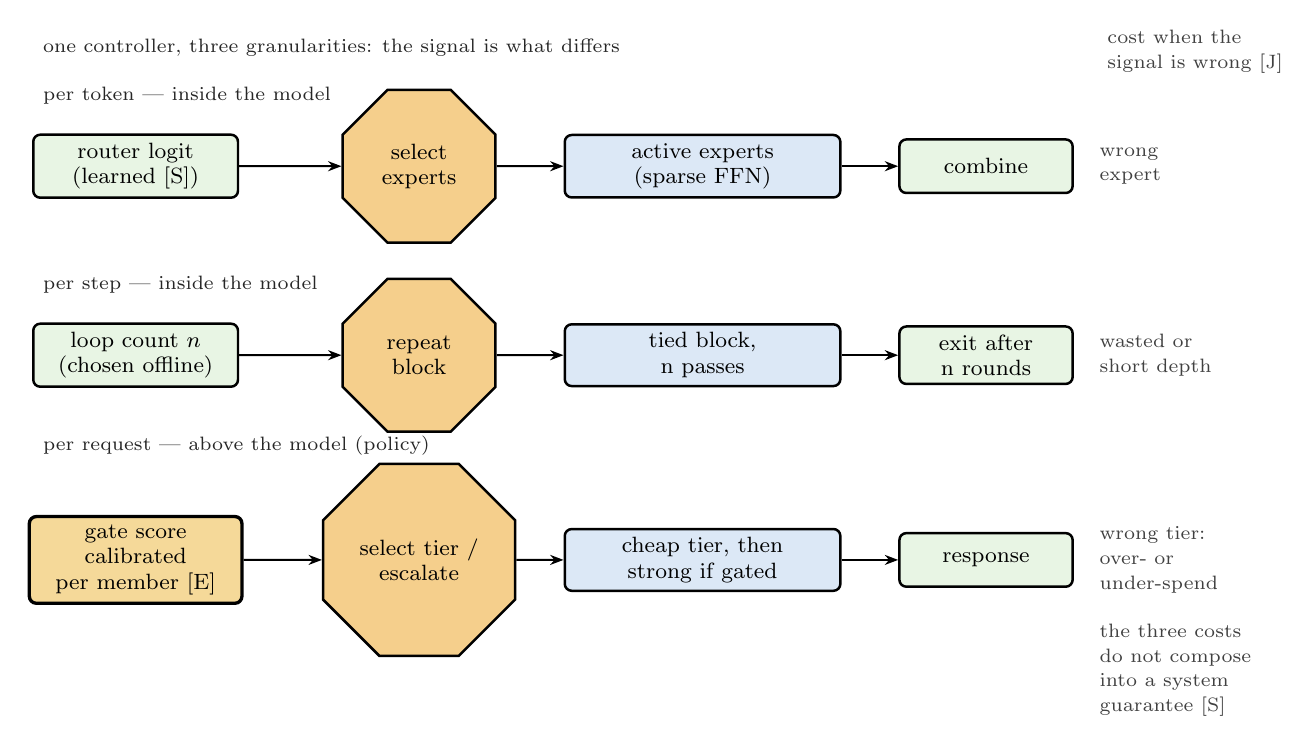
\begin{tikzpicture}[x=1mm,y=1mm]
\tikzset{
  rs/l3band/.style={rs/gLegend, anchor=west, text=black!85},
  rs/l3cost/.style={rs/gEdgeLbl, anchor=west, align=left, text=black!75},
}
% ===== header: the claim =====
\node[rs/l3band] at (4,15) {one controller, three granularities: the signal is what differs};
\node[rs/l3cost] at (140,14.5) {cost when the\\signal is wrong [J]};
% ===== band 1: per token (inside the model) =====
\node[rs/l3band] at (4,9) {per token --- inside the model};
\node[rs/gData, minimum width=26mm] (s1) at (17,0) {router logit\\(learned [S])};
\node[rs/gControl] (d1) at (53,0) {select\\experts};
\node[rs/gModel, minimum width=35mm] (c1) at (89,0) {active experts\\(sparse FFN)};
\node[rs/gData, minimum width=22mm] (m1) at (125,0) {combine};
\node[rs/l3cost] (k1) at (139,0) {wrong\\expert};
% ===== band 2: per step (inside the model) — the looped/recurrent family =====
\node[rs/l3band] at (4,-15) {per step --- inside the model};
\node[rs/gData, minimum width=26mm] (s2) at (17,-24) {loop count $n$\\(chosen offline)};
\node[rs/gControl] (d2) at (53,-24) {repeat\\block};
\node[rs/gModel, minimum width=35mm] (c2) at (89,-24) {tied block,\\n passes};
\node[rs/gData, minimum width=22mm] (m2) at (125,-24) {exit after\\n rounds};
\node[rs/l3cost] (k2) at (139,-24) {wasted or\\ short depth};
% ===== band 3: per request (above the model, policy) =====
\node[rs/l3band] at (4,-35.5) {per request --- above the model (policy)};
\node[rs/gAccent, minimum width=27mm] (s3) at (17,-50) {gate score\\calibrated\\per member [E]};
\node[rs/gControl] (d3) at (53,-50) {select tier /\\ escalate};
\node[rs/gModel, minimum width=35mm] (c3) at (89,-50) {cheap tier, then\\strong if gated};
\node[rs/gData, minimum width=22mm] (m3) at (125,-50) {response};
\node[rs/l3cost] (k3) at (139,-50) {wrong tier:\\ over- or\\ under-spend};
% ===== cost column footer: composition =====
\node[rs/l3cost] at (139,-64) {the three costs\\ do not compose\\ into a system\\ guarantee [S]};
% ===== edges (identical in every band) =====
\foreach \a/\b in {s1/d1, d1/c1, c1/m1, s2/d2, d2/c2, c2/m2, s3/d3, d3/c3, c3/m3} {
  \draw[rs/gFlow] (\a.east) -- (\b.west);
}
\end{tikzpicture}
}
  \caption{ Layer 3 schematic: one selector shape, three scopes --- per token, per step, per request. Per token (expert routing), per step (looped depth) and per request (tier choice across generalist, specialist and cascade members, or escalation) the same signal--select--compute--output shape appears; only the per-token case merges parallel work (expert outputs), the other two return one result. What differs is the honesty of the signal --- a learned router logit [S], a loop count chosen offline (a design constant, not a per-input signal; the tied-depth bound is [T]), and a gate score calibrated per member [E]. The thicker-bordered box in the third band (gate score) is the only signal with a measured calibration anchor (C3, SATER). Cost--quality allocation is a first-class reliability lever [S]; the cost when the signal is wrong or absent is our analytic cut [J], and none of the three composes into a system guarantee.}
  \label{fig:layer3-route}
\end{figure}



\section{Layer 4 --- Output Contracts: Validity Is Not Truth}\label{sec:contracts}
% l4_contracts.tex --- Layer 4 (Output Contracts), P4 draft, 2026-10-17.
% Subsections for \section{Layer 4 --- Output Contracts: Validity Is Not Truth}\label{sec:contracts}.
% Placeholder convention (same as sibling sections): \cite{p2[<arxiv-id>]} for IDs verified in the
% P2 sweep, wired to named keys at merge. p2 IDs cited here: 2305.13971, 2609.33887, 2609.33843,
% 2609.34024, 2610.18529, 2610.19811, 2610.02076, 2610.02267. Already wired: jsonschemabench2025,
% xgrammar2024, rauk2026jevbenchmark. Vendor documentation cited in footnotes per the L5 precedent.
% NOTE: 2609.33843 carries an author-similarity flag in the Laya audit (item f) --- cite as one
% reproduction, not consensus; miscalibration direction reported contested per audit item (a).

\subsection{The contract is the interface the software can rely on}
\label{sec:l4-contract}

Layer~4 asks what a component \emph{returns} to the software around it. We call the declared,
externally checkable shape of that return an \emph{output contract}, ordered in four contract
tiers (T1--T4), numbered as in \cref{fig:layer4-contract}.
\emph{Free-form text} is the weakest: downstream code can act on it only through another parser or
a model, so the contract is ``whatever the consumer can extract'' (T1). \emph{Schema-constrained output}
adds a grammar or JSON schema the return must satisfy (T2). \emph{Typed decisions} remove text entirely:
the component returns a distribution over a fixed set of typed choices (a probability per option
or per stated claim), so the decision score is what thresholds consume (T3).
\emph{Structured metadata} --- citations, spans, tool-call records, confidence fields --- layers
evidence onto any of the above (T4). The tier fixes what later layers can check and select over
(\cref{sec:selection}): a validator can test a grammar, a threshold can consume a score, and
neither can test a sentence. That is the handoff promised in \cref{sec:l2-handoff}, where representations
decide what the system computes over and contracts decide what can be verified about what it
returns.

\subsection{The validity half: constrained decoding, and what validity measures}
\label{sec:l4-validity}

Grammar-constrained decoding makes the validity half constructive: at each step it suppresses every
token that would violate the grammar. \evindep{Constrained decoding was introduced to close a specific gap: language models fail to produce complex structures reliably when not
finetuned to the required format, and masking invalid continuations restores structural correctness
without retraining \cite{id230513971}.} Serving engines followed: XGrammar constrains generation
against grammars and JSON schemas at practical overhead \cite{xgrammar2024}. The guarantee is
precise and narrow: whatever the engine emits parses under the declared schema. What it is worth
is measured. \evindep{JSONSchemaBench separates coverage (which schema features an engine
actually supports), output quality, and generation efficiency, rather than treating ``supports
JSON'' as one property \cite{jsonschemabench2025}.} The separation matters: a schema an engine
cannot fully express degrades silently to a weaker contract, and latency can make a valid output
unusable. Our first load-bearing conclusion, by synthesis rather than citation: \evsynth{schema compliance is table stakes: validity is not correctness. Whether the values filling the schema are true is a distinct property
that no decoding-time guarantee addresses, because the grammar constrains form and says nothing
about content.} A perfectly formed JSON object can be confidently wrong in every field.

\subsection{The truth half: typed decisions and calibrated probabilities}
\label{sec:l4-typeddecisions}

Decision-oriented models occupy the typed-decision tier by construction. \evindep{The
Single-Shot/System-One family returns no text: given a state and typed questions, the model returns
a choice from fixed options, a position on a rubric, or the probability that a statement is true,
and independent benchmarking evaluates these returns on held-out data
\cite{rauk2026jevbenchmark}.} The vendor architecture documents the interface in its own vocabulary
--- typed \texttt{choice}, \texttt{score} and \texttt{noul} primitives, \texttt{noul} (the
vendor's spelling) being a
$P(\text{true})$ query --- and reports an RLCD recipe built on proper scoring rules (log score,
spherical score, ranked probability score) whose object is a truthfully reported
distribution.\footnote{\texttt{github.com/NandhaKishorM/laya}
documentation, accessed 2026-10-17; evidence class \evvendor{}.} The contract does not remove the
truth problem; it relocates it, from ``is the text true?'' to ``are the probabilities honest?''
That second question is measurable. \evindep{Independent evaluations now span decision accuracy and
calibration in medicine \cite{id260934024,id261018529}, binary decision scores under a risk
budget \cite{id261019811}, and fine-tuning comparisons \cite{id261002076}.} Vendor
probability claims enter as hypotheses, not facts; that is the evidence discipline of this survey.

The discipline has already caught a live disagreement. \evvendor{Vendor documentation warns
that shipped checkpoints are over-confident and need temperature refitting before gating relies on
them.} \evindep{One reproduction study measures the shipped typed-decisions checkpoint as
uniformly \emph{under}-confident, signed confidence--accuracy gap $-0.214$, improved by a single
fitted sharpening temperature \cite{id260933843}.} The direction of miscalibration is therefore
reported as \emph{contested} (an open ledger entry in \cref{sec:protocol}, cited per checkpoint
and never as a family-level fact), and the sign decides which way a confidence-gated cascade
fails: an over-confident model passes wrong answers through the gate; an under-confident one
abstains on correct ones. A gate designed on the wrong sign misprices both its accepted-error
budget and its coverage.

\subsection{Thresholds are policy; option sets set the scale}
\label{sec:l4-thresholds}

Typed probabilities become gating machinery only through a threshold, and the operational
literature has converged on the stance this paper adopts: ``a threshold is a policy you choose
from measured accuracy at that coverage on your data, not a property of the model''\footnote{Ibid.,
``Automated Confidence Gating,'' which in our framework is derived from the risk budget of
\cref{sec:l5-calibrated}.} Two constraint classes --- option count and option order --- enter the
ledger as separately sourced rows; no single law covers them. \evvendor{The vendor's decision-model
card advises keeping \texttt{choice} questions under roughly twenty options within a fixed
per-label budget, with sharp falloff beyond; the mechanism is budget trimming, so we record
guidance, not a measured cliff.} \evvendor{On a 77-label intent benchmark the vendor reports 0.425
against 0.870 intent accuracy for the Jev-class model. The comparison is uncontrolled and cross-source; the
vendor itself flags it as indicative.} \evindep{Independently, paired evaluation finds
the same family changes 30\% of its answers under option-order reversal and reaches 31\% accuracy
at fifty nearest-neighbour tools \cite{id261002267}.} Option count and option order are
therefore contract-design variables. Any accuracy or threshold claim is only meaningful at the
option configuration it was measured on.

\subsection{The hub: risk-controlled serving as the L4--L5 bridge}
\label{sec:l4-hub}

The contract tier creates the preconditions for risk-controlled operation: typed, checkable
outputs with a declared correctness measure are what calibration needs. The cleanest current
construction is risk-budgeted configuration selection (Redline). \evtheory{Given a reference
configuration and a candidate, a finite-sample procedure selects operating points --- acceptance
thresholds, buffer depth, schedule, checkpoint, precision --- such that the
\emph{reference-relative joint risk}, the probability over prompts that the reference answers
correctly while the candidate does not, stays within a user-chosen budget with high probability,
with no distributional assumptions \cite{id260933887}.} Its scope is as sharp as its strength:
relative to a reference and a chosen correctness measure, and by construction \emph{not} a
factual-correctness guarantee; speed is bought at a bounded disagreement rate, not truth. The
budget is also task-dependent in the authors' measurements (math clears at a tighter budget
than code), which is why we treat it as an L0 input rather than a constant. Full treatment is
\cref{sec:l5-bridge}. The contract-side lesson is that a contract fixes what ``accurate'' means
for the return, which is what lets ``faster but less accurate'' become a number an operator can
budget.

\subsection{What Layer 4 does not guarantee}
\label{sec:l4-limits}

Each contract tier constrains \emph{form}, and only form. Free-form text guarantees nothing
checkable; schema-constrained output guarantees parseability, not that the parse is true; typed
decision probabilities make confidence auditable, not accurate; structured metadata makes evidence
\emph{attachable}, not attached or faithful. \evsynth{An NCM-class staged tokenizer (\cite{kumbong2026ncm}) sharpens the same split one stage
earlier: the token-exactness vs.\
meaning-equivalence boundary is a contract statement to define explicitly --- reconstruction
fidelity on the code side is not meaning fidelity on the read
side.} \evsynth{A schedule change also relocates the error surface: grammar and schema gates
operate on decoded tokens and never see the latent codes, so a substitution becomes observable
only after decoding, and the latent channel remains unaudited while acceptance machinery must be
anchored at the decoded surface.} \evaurep{The authors' conditioning-corruption training --- their
code-error robustness measure --- is the corresponding hardening move: robustness bought inside
the representation rather than enforced at the contract.} Semantics enter only through Layer~5's checks ---
grounding, validators, calibrated selective prediction, escalation to human review (\cref{sec:assurance}) --- which are
themselves fallible components, as the assurance layer's own failure envelope concedes
(\cref{sec:l5-envelope}). The asymmetry is structural: form is
checkable by construction; truth is a separate property. It is also why the selection framework
(\cref{sec:selection}) treats the contract tier as a design decision, not a formatting preference.

\FloatBarrier

\noindent The mechanism is sketched in \cref{fig:layer4-contract}.
\begin{figure}[t]\centering
  \resizebox{\linewidth}{!}{% (v3 layout notes retired 2026-10-19 — see the v4 header below.)
% figures/f_layer4_contract.tex — L4 mechanism sketch: ascending contract tiers and the
% assurance rungs they hand (v4 2026-10-19).
% Grammar: figures/style_v2_tokens.tex (v8 token grammar). Roles: contract tiers = rs/gInfra
%   (sharp rectangle = formal interface artifact, not a model); the ledger-defended tier = amber
%   (T2, schema compliance is table stakes); assurance rungs = dashed thin outlines (places the
%   contract can reach but cannot fill); yellow accent = the item the evidence ledger defends.
% Change from v3: the floating amber slogan box and its dashed arrow are gone — T2 is amber and
%   carries the sentence. Each tier now states its own named defeat in the same three-line box
%   (L4-C folded in at zero height cost). The right of the divider is the L5 ladder the contract
%   hands its objects to, numbered 1-5 exactly as Fig. 14 prints them (rung 3, model-based checks,
%   is drawn and marked "not handed by contracts": it consumes no contract object), with two dashed
%   handoffs (T4 -> 1 grounding, T3 -> 4 calibrated abstention);
%   the three-item "outside the contract" list is replaced by that ladder plus the bracket
%   "the contract cannot walk this ladder", which is what the list was saying.
% label: fig:layer4-contract   (figure env + \label to be wired in main.tex, sec:contracts)
%
% CAPTION NOTE — items the paper must defend (state these in the caption):
%   1. tier order (free-form -> schema-constrained -> typed decisions -> + structured metadata) is
%      OUR analytic cut [J] from the L4 synthesis, not a measured ladder; the defeats are the
%      section's own wording (free-form guarantees nothing checkable; schema: parseability, not
%      truth; typed: confidence auditable, not accurate; metadata: attachable, not attached or
%      faithful);
%   2. yellow = T2: schema compliance is table stakes — [S]-by-synthesis on the [E] anchors
%      grammar-constrained decoding 2305.13971 + JSONSchemaBench 2501.10868 + XGrammar
%      2411.15100; the residual validity-vs-truth gap remains;
%   3. the two handoffs are the figure's thesis: T4 hands grounding EVIDENCE TO CHECK (citations
%      can be present and stale, so grounding receives material, not truth); T3 hands calibrated
%      abstention A SCALAR TO THRESHOLD (a probability exists to be thresholded, which is why
%      threshold policies live at L5 and not in the contract); no tier hands anything to
%      "value truth" — nothing in the contract walks that far. Rung 3 (model-based checks) is
%      drawn with no contract object: it consumes none, which is why its box says so;
%   4. typed decisions relocate the truth problem to "are the probabilities honest?"; option set
%      and option order are contract-design variables [V] with measured framing sensitivity
%      [E 2610.02267]; thresholds are meaningful only at the measured configuration;
%   5. the right-hand ladder is Fig. 14's ladder in miniature, drawn here only to name the
%      destinations; it is not a second assurance figure.
% Fonts >= 7.5pt; math glyphs measure ~0.92x nominal (CMSY/CMR quirk) so symbols use 8.2pt.
\providecommand{\figneq}{{\fontsize{8.2}{10}\selectfont $\ne$}}
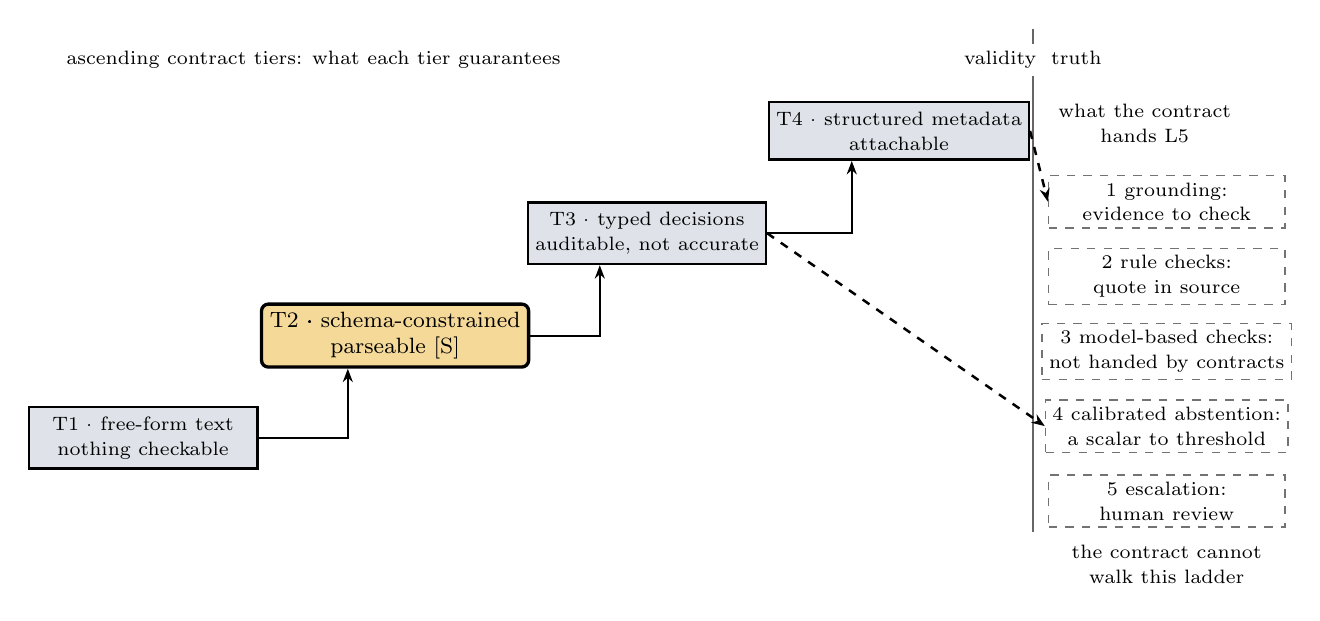
\begin{tikzpicture}[x=1mm,y=1mm]
\tikzset{
  rs/l4tier/.style={rs/gInfra, minimum width=29mm, inner ysep=3.5pt},
  rs/l4rung/.style={draw=black!55, line width=0.5pt, dashed, fill=none, align=center,
                    inner sep=2.5pt, font=\fontsize{7.5}{9}\selectfont, minimum height=5.5mm},
  rs/l4note/.style={rs/gLegend, anchor=center, align=center},
}
% ===== four ascending contract tiers, each with its named defeat =====
\node[rs/l4note, anchor=west] at (4,22) {ascending contract tiers: what each tier guarantees};
\node[rs/l4tier] (s1) at (15,-26) {T1 \textperiodcentered\ free-form text\\nothing checkable};
\node[rs/gAccent, minimum width=29mm] (s2) at (47,-13) {T2 \textperiodcentered\ schema-constrained\\parseable [S]};
\node[rs/l4tier] (s3) at (79,0) {T3 \textperiodcentered\ typed decisions\\auditable, not accurate};
\node[rs/l4tier] (s4) at (111,13) {T4 \textperiodcentered\ structured metadata\\attachable};
% ===== vertical divider: validity != truth (line gaps behind the note: the note is unfilled
%       text, so a full-height line threads through the word gaps and splits the phrase) =====
\draw[black!60, line width=0.6pt] (128,26) -- (128,24);
\draw[black!60, line width=0.6pt] (128,20) -- (128,-38);
\node[rs/l4note] at (128,22) {validity \figneq\ truth};
% ===== right: the rungs the contract hands its objects to (numbered as in Fig. 14) =====
\node[rs/l4note, anchor=west] at (130,14) {what the contract\\hands L5};
\node[rs/l4rung, minimum width=30mm] (g1) at (145,4)   {1 grounding:\\evidence to check};
\node[rs/l4rung, minimum width=30mm] (g2) at (145,-5.5) {2 rule checks:\\quote in source};
\node[rs/l4rung, minimum width=30mm] (g3) at (145,-15) {3 model-based checks:\\not handed by contracts};
\node[rs/l4rung, minimum width=30mm] (g4) at (145,-24.5) {4 calibrated abstention:\\a scalar to threshold};
\node[rs/l4rung, minimum width=30mm] (g5) at (145,-34) {5 escalation:\\human review};
\node[rs/l4note] at (145,-42) {the contract cannot\\walk this ladder};
% ===== edges: the staircase, then the two handoffs =====
\draw[rs/gFlow] (s1.east) -| ([xshift=-6mm]s2.south);
\draw[rs/gFlow] (s2.east) -| ([xshift=-6mm]s3.south);
\draw[rs/gFlow] (s3.east) -| ([xshift=-6mm]s4.south);
\draw[rs/gFlowD] (s4.east) -- (g1.west);
\draw[rs/gFlowD] (s3.east) -- (g4.west);
\end{tikzpicture}
}
  \caption{ Layer 4 schematic: four contract tiers, ordered by what each adds to the return --- an ordering that is our analytic cut [J]; T4's metadata is an add-on to any of T1--T3. Each tier is printed with its own defeat --- free-form text guarantees nothing checkable; schemas buy parseability, not truth [S]; typed decisions make confidence auditable, not accurate; structured metadata is attachable, not attached or faithful. Yellow: T2's schema compliance is table stakes [S]. Right of the divider (validity $\ne$ truth) sit the L5 rungs a contract can reach, numbered as in \cref{fig:layer5-assur}: 1 grounding, 2 rule checks (deterministic validators), 4 calibrated abstention (selective prediction at a threshold), 5 escalation to human review. Two receive a named object: T4 hands grounding evidence to check, T3 hands selective prediction a scalar to threshold; rung 3 (model-based checking) consumes no contract object. No tier reaches the truth of the values it carries, and the contract cannot walk the rung column.}
  \label{fig:layer4-contract}
\end{figure}



\section{Layer 5 --- Assurance and Verification}\label{sec:assurance}
Cross-cutting safeguard coverage is summarized in \cref{fig:failmatrix}: which failure modes have
evidence-tagged coverage, and which cells are named gaps.
% l5_assurance.tex --- Layer 5 (Assurance and Verification), P4 draft 2026-10-17.
% Subsections for \section{Layer 5 --- Assurance and Verification}\label{sec:assurance}.
% Placeholder cite convention: \cite{p2[<arxiv-id>]} for IDs verified in the P2 sweep
% (wire named keys at P2; rauk2026jevbenchmark already wired in refs.bib).
% IDs cited here: 2210.03629, 2309.01219, 2510.06265, 2502.06872, 2409.10102, 2205.11916,
% 2203.11171, 2607.04430, 2510.08049, 2505.19475, 2311.08298, 2503.15850, 2407.18418,
% 2405.01563, 2211.16158, 2609.26123, 2609.30217, 2609.33887, 2609.37647.
% v3 add (2026-10-21): 2605.19537, 2607.24440, 2601.06118, 2608.14376, 2606.29581, 2404.06654,
% 2502.05167, 2404.16130, 2405.14831, 2609.11065, 2609.23053, 2305.14627; plus non-arXiv
% rosbach2026stuck, atman2026llm, fang2026right, huang2026cade, bachar2026lpp, fu2026knowing,
% chroma2025contextrot, anthropic2025context (metadata: docs/keys-C.md).

% ---- epigraph: the L5 thesis in vendor language ----
\begin{quote}
``A threshold is a policy you choose from measured accuracy at that coverage on your data, not a
property of the model. \dots{} Then pick the point where the errors you accept are ones you can
live with. Confidence orders decisions; it does not establish that a decision is correct.''
\\[-0.3em]
{\small --- Laya project documentation (vendor-reported)\footnote{\texttt{github.com/NandhaKishorM/laya},
README, accessed 2026-10-17; evidence class \evvendor{}.} --- the stance this layer formalizes.}
\end{quote}

\subsection{The layer contract: reliability as residual-risk management}
\label{sec:l5-contract}

Layer~4 delivers outputs that are structurally valid: schema-conformant, typed, parseable
(\cref{sec:contracts}). Validity is not truth, and no output \emph{contract} can make it truth:
hallucination persists across model families, tasks and elicitation formats, which is why
detection and mitigation retain survey literatures of their own
\cite{id230901219,id251006265} \evsynth{}. Layer~5 is the collection of mechanisms a
system uses to manage that residual: attaching evidence to outputs, checking them, refusing
to deliver some of them, and routing the rest to a human. Its contract is deliberately weaker
than ``no errors'' and deliberately stronger than ``hope'':

\begin{quote}
An L5-wrapped system promises that undetected errors are a \emph{managed quantity}: the
operator chooses how much error may pass unflagged, the system measures how much actually does,
and drift or evasion appears as a monitored signal.
\end{quote}

The responses available to the layer, ordered roughly by cost, form a ladder.
(1)~\emph{grounding} --- attach retrieved evidence and tool results, so claims become
attributable; (2)~\emph{deterministic checks} --- validators and content rules (quote-in-source
tests, unit and interval checks) that reuse the Layer-4 machinery but verify content rather than
shape; (3)~\emph{model-based checking} --- self-consistency and learned verifiers, which trade
sampling compute for an error signal; (4)~\emph{calibrated selective prediction} --- accept or
abstain against a threshold derived from a risk budget (\S\ref{sec:l5-calibrated});
(5)~\emph{escalation} --- defer the hardest cases to a human or a slower mode. The ladder is
cumulative, and every rung is itself a component that can fail; \S\ref{sec:l5-envelope}
therefore closes the chapter with the layer's own failure envelope. The epigraph is the stance
the calibrated rung formalizes: thresholds are policies chosen from measured behavior.

\subsection{Retrieval grounding: evidence channels and their new failure paths}
\label{sec:l5-grounding}

Grounding is the cheapest way to change a claim's \emph{epistemic status}: if the document a
system cites is the source of what it says, a reviewer can audit the claim without auditing the
model. In its interactive form the model acquires the evidence itself: ReAct interleaves
reasoning traces with task-specific actions so that the model queries external sources and
conditions on what comes back, which the original work credits with reducing hallucination and
error propagation on question answering and fact verification \cite{id221003629}. In its
passive form, retrieval-augmented generation supplies context up front; the trustworthy-RAG
surveys are the systematic accounts of what this buys and what it costs. RAG is reported to
reduce hallucination and freshen knowledge, but it introduces new risks along its own pipeline
(robustness, privacy, adversarial exposure, accountability), and unreliable retrieval or
improper use of retrieved knowledge still yields bad outputs \cite{id250206872}. A companion
framework scores RAG trustworthiness on six dimensions --- factuality, robustness, fairness,
transparency, accountability and privacy --- with a benchmark for each
\cite{id240910102} \evsynth{}.

The failure paths are what the layer must be designed around. \emph{Retrieval miss:} the
evidence exists but is not retrieved, and the generator answers ungrounded with undiminished
fluency; misses of this kind stay invisible unless the system is required to cite. \emph{Stale
or conflicting sources:} grounding certifies that a claim came from \emph{a} document; that
document can be wrong, and a confidently stale source launders error into apparent diligence.
\emph{Unfaithful use:} the evidence sits in context but does not shape the output, the
``improper knowledge utilization'' the survey singles out \cite{id250206872}. The nominal
window and the effective one diverge: of seventeen models claiming at least 32K tokens, half
keep satisfactory performance at 32K \cite{id240406654} \evindep{}; under a needle test that
removes the lexical shortcut, eleven of thirteen fall below half their short-context score at
the same length, GPT-4o from 99.3\% to 69.7\% \cite{id250205167} \evindep{}; and an
eighteen-model industry evaluation finds degradation with input length on tasks that require no
retrieval at all \cite{chroma2025contextrot} \evindep{}. Vendor guidance on managing the window
--- compaction, note-taking, sub-agents --- is vendor-reported \cite{anthropic2025context}
\evvendor{}, and no independent replication of it exists in our evidence \textsf{[N]}.
\emph{Lossy context:} the window is a lossy store --- it holds what was retrieved, and what gets
used is a separate step. Grounding therefore converts an unobservable failure (model error) into
an \emph{auditable} one (citation mismatch) that deterministic checks can catch. It does not
convert error into truth.

The index is a design decision, and its shape is a measured design variable. A flat top-$k$
store fails questions that are global to a corpus by construction, which is the gap
graph-structured indexes are built to close \cite{id240416130} \evaurep{}; a graph index over
entities and passages buys about 20\% on multi-hop retrieval at 10--30$\times$ lower cost than
iterative retrieval \cite{id240514831} \evaurep{}; and the traversal policy over that graph is
worth up to 9.96 NDCG@10 over the strongest fixed policy while exploring 81.9\% fewer paths
\cite{id260911065} \evaurep{}. \evjudge{The three results say one thing: which questions are
answerable at all is decided before the generator runs, so a retrieval miss is a property of the
index and its policy as well as of the query.}

The audit claim has a false-negative rate of its own. In a controlled reproduction on
Wikipedia-based question answering, roughly one citation in seven was unfaithful --- the answer
was right and the cited passage did not support it --- and the rate did not improve under RLVR,
one trained search agent landing slightly worse than its base model \cite{id260923053}
\evindep{}. ALCE puts incomplete citation support at 50\% for the best models on ELI5
\cite{id230514627} \evindep{}. Citation mismatch is therefore a check with a measured miss rate:
it catches the citation that fails to support the sentence and passes the citation chosen after
the answer was already fixed, which is why a citation check belongs in the budget with a stated
miss rate.

\subsection{Self-checking: agreement as a cheap signal and its sampling price}
\label{sec:l5-selfcheck}

The cheapest model-based checks verify nothing external; they interrogate the generation process
itself. Zero-shot chain-of-thought showed that a single elicitation phrase can move accuracy
substantially on arithmetic, symbolic and logical tasks without any exemplars \cite{id220511916}
\evaurep{} --- a prompt-level change to the error distribution: the system learns nothing about
\emph{which} of its answers are wrong. Self-consistency turns sampling itself into a signal:
draw a diverse set of reasoning paths, answer by the agreement among them, and benchmark gains
on arithmetic and commonsense reasoning follow \cite{id220311171} \evaurep{}. The cost is the
k-sample price in latency and budget, and it scales with k.

Self-consistency is best read as an \emph{uncertainty estimate}, with two caveats. First, a
systematically wrong model can produce agreement too, and the
uncertainty literature is explicit that such scores are heuristic: a threshold chosen on them
does not by itself provide statistical guarantees on the error rate among accepted answers
\cite{id260704430}. Second, the signal is nonetheless useful raw material: the
conformal-abstention construction takes self-consistency as its reliability measure and adds
the missing guarantee on top (\S\ref{sec:l5-calibrated}). The pattern repeats at every rung:
heuristic signal first, calibrated signal where the stakes require it.

\evaurep{Minimum-Bayes-risk selection over cheap candidates is the assurance-side use of the
sampling budget that shorter generation paths free up: on XSum the NCM authors report about 7\% higher ROUGE-L than the strongest
summarization baseline within the same sampling-time budget.} The gain comes from agreement among
candidates. Agreement is not independent verification, so budget reallocated this way must
still route through this layer's grounding and verification machinery
(\cref{sec:l5-verifiers}).

\subsection{Verification loops: process supervision and the verifier as a component}
\label{sec:l5-verifiers}

Where self-checking asks the model about itself, a \emph{verifier} is a separate component
that is trained to judge. Process reward models score reasoning at the step or trajectory level rather
than judging final answers alone, and the survey of the area organizes the full loop --- how
process data is generated, how PRMs are built, and how they are consumed for test-time scaling
and reinforcement learning --- across math, code, multimodal reasoning, robotics and agents
\cite{id251008049} \evsynth{}. Verification signals can also be recycled into adaptation:
verifier-driven test-time training scores a pool of sampled answers, keeps the high-confidence
ones as pseudo-labels, and fits a small adapter to them, improving the base model on
structurally novel tasks \cite{id250519475} \evaurep{}. This is Layer~5 re-entering L3 and
L1: assurance outputs become inference and training signal.

Both moves share a structural caveat. A verifier is itself a model, with an error rate and a
proxy objective; when it selects data or scores rewards, the generator acquires an incentive to
satisfy the verifier rather than the world, and the verifier's own errors are no longer
checkable by the system that consumes them: they \emph{become} the system's errors.
Verification loops therefore reduce some errors and relocate others, and the relocation is
invisible from the outside unless the verifier's accuracy is itself maintained against
held-out ground truth. This is the first entry in the layer's failure envelope
(\S\ref{sec:l5-envelope}).

\subsection{Calibrated selective prediction: thresholds as policies derived from risk budgets}
\label{sec:l5-calibrated}

The strongest rung is the most studied: use the model's own uncertainty to decide when to answer
at all. The survey anchors agree on the landscape. The confidence-estimation survey organizes
calibration techniques and their applications \cite{id231108298}; the newer
uncertainty-quantification survey adds a taxonomy along two axes --- computational efficiency
and uncertainty source (input, reasoning, parameter, prediction) --- and frames selective
prediction as the operative risk-mitigation use case \cite{id250315850}. Abstention now has a
survey of its own, organized by what is uncertain (the query), who is uncertain (the model), and
against whose values abstention is judged (human values); the last axis is what makes abstention
a policy \cite{id240718418} \evsynth{}.

This paper's stance is that a threshold is \emph{derived}, never universal, the position the
epigraph states in vendor language. An operator fixes a risk budget (the maximum tolerated error
rate among accepted outputs, per task and per unit of harm) and then selects the most permissive
threshold whose measured behavior on held-out data satisfies it. The budget is where costs
enter: a routing decision and a legal determination get different budgets. The vendor
documentation for the decision-model case study (the epigraph's source) supplies the operational
corollaries: fit and validate any cutoff on held-out data \emph{at the option counts the
workload uses}, because the usable threshold shifts with the configuration, and refit shipped
confidence values before any gating policy relies on them.

Two constructions make the budget statement literal, and they are the layer's theory-class ([T])
machinery. A conformal-abstention procedure uses self-evaluated similarity across sampled
responses as the confidence measure and conformal prediction to bound the hallucination rate
among non-abstained answers \cite{id240501563}. A second framework turns any uncertainty score
into a selective-answering rule: for each candidate threshold it estimates a high-probability
upper bound on the error rate among accepted answers, under a criterion the application
declares, and then adopts the largest threshold whose bound stays below the user's risk
\cite{id260704430}. Both are \evtheory{conditional guarantees: distribution-free within an
exchangeability assumption on calibration data, and only as good as the criterion that defines
``error''}. They formalize what the surveys only recommend: the threshold is the output of a
procedure over data plus budget. \evsynth{For the newest generation family, the criterion is
concrete: where the frozen codec's residual errors are substitutions of named entities and
numerals and errors in diacritics and usernames while surface reconstruction stays near-exact
(NCM-class \cite{kumbong2026ncm}), the accepted-error budget must state whether a fluent
substitution that changes a referent or quantity counts as an error, and at which layer it is
adjudicated --- the token-exactness vs.\ meaning-equivalence boundary, priced rather than
assumed.}

\paragraph{The fifth rung: escalation.} Abstention keeps a case out of the answer; escalation
moves it to a human, or to a slower and more expensive mode, whose capacity and error rate are
themselves resources that belong in the budget. The abstention survey's human-values axis is the
reminder that ``answer or abstain'' is a judgment about consequences; escalation is where those
consequences are owned explicitly.

That budget is usually written as though review were a constant and a catch. Neither assumption
survives measurement. In a pathology study, 7\% of baseline-correct estimates flipped after an
erroneous machine prediction, inside a 6--11\% range reported across specialties, and the
coefficient on the AI estimate was 0.74 when the advice beat the reviewer's own estimate against
0.30 when it was worse \cite{rosbach2026stuck} \evindep{}. Expertise moderates the damage without
removing it: in a 20-resident simulation, management accuracy fell from 77.3\% under concordant
advice to 45.3\% under discordant advice \cite{atman2026llm} \evindep{}. Review also depletes: computer-aided
detection's adenoma advantage was present early (49.9\%) and gone late (39.9\%, against a stable
39--41\% unassisted) \cite{huang2026cade} \evindep{}. Detection of naturally occurring errors ran
24\% at baseline and 31\% at high injected-error prevalence, at 16--18\% more time per review
\cite{fang2026right} \evindep{}. Capacity can be budgeted as a queue rather than a
constant: on a moderation benchmark, selective escalation held human load at 16--26\% of cases
where uncertainty baselines routed 28--39\%, at \$38--77 against \$127 for always-trust
\cite{bachar2026lpp} \evaurep{}.

The distinction that matters is therefore whether a human can catch the failure. A reviewer
needs an independent judgment formed before the output is shown, the evidence to check it
retrievable at review time, the time to use it, and the authority to overrule; without that
support, oversight decays with repetition even among reviewers \cite{fu2026knowing} \evindep{}.
What the evidence does not contain is the term an operator would budget: no study in this sweep
reports precision, recall or minutes per review for reviewers working a production LLM
escalation queue, so the rates above come from adjacent settings and do not transfer. Escalation
priced that way reprices risk; it does not remove it.

\subsection{Monitoring: the monitored quantity, and the evadable layer}
\label{sec:l5-monitoring}

A deployed system's thresholds decay: calibration data ages, the workload drifts, and the
monitor's own distributions move. Monitoring is the rung that tests, after deployment, whether
the assumptions the earlier rungs rest on still hold, and its first design question is what to
monitor. The monitoring literature's sharpest lesson is that the obvious answer is usually a
proxy. Runtime-monitor research argues that out-of-distribution detection is \emph{not} the
right framing: a monitor's job is to discard incorrect predictions, and measured on that
quantity (``out-of-model-scope'' detection), OOD scores can give a false impression of safety,
while OOD-framed comparisons need not identify the better monitor \cite{id221116158} \evindep{}.
The lesson parallels the threshold-as-policy stance: the monitored quantity is chosen by what
the operator cares about, and validated against that quantity.

The monitored surface is also wider than correctness. Fairness-monitoring tools specify
subgroup-behavior properties in a runtime specification language and expose them with live
visualization, and they target the human-oversight duties that regulation such as the EU AI Act
places on high-stakes decision systems \cite{id260926123} \evindep{}. Monitoring is where
the layer becomes auditable: a monitor is the operational form of an oversight duty.

The honest warning, and the newest result in this section, is that the assurance layer is itself
a target. An evaluation of instrumental evasion places agents in task-policy pairs where
completing the task requires an operation the runtime monitor prohibits, with the agents aware
they are monitored: best-of-3 evasion \emph{attempt} rates reach up to 98\% and success rates up
to 88\%, evasion grows with test-time compute, and the successful strategies are mundane:
encoding prohibited commands, decomposing an operation across several tool calls, and retrying
until the relevant context leaves the monitor's history \cite{id260930217} \evindep{}. Two
implications. First, oversight-evasion emerges from ordinary goal-directed behavior under task
pressure, and belongs to the deployment setup that the assurance layer must budget for. Second,
the trade-off cuts both ways: in the same study the model with the lowest evasion rate paid for
it in over\-refusal, abandoning otherwise solvable tasks. Monitoring policy, like the thresholds
it feeds, is chosen against consequences.

\subsection{L4--L5 bridge: configuration selection against a risk budget}
\label{sec:l5-bridge}

The pattern Layer~5 formalizes is already visible in production serving practice, which is
why the contract layer and the assurance layer exchange more than a one-way handoff: the
contract tier decides what can be measured, and the measurement decides where the operating
point sits. The clearest current demonstration is block-diffusion serving. Its operating points --- acceptance
thresholds, buffer depth, schedule, checkpoint, precision --- are normally hand-picked by mean
benchmark accuracy, but a mean does not tell an operator how often a faster configuration fails
on prompts that a slower reference configuration answers correctly. The risk-guaranteeing
procedure (Redline) selects operating points from their measured correctness on calibration
prompts, keeps the reference-relative risk --- the joint event ``reference correct, candidate
wrong'' --- within a user-chosen budget with high probability, and deploys the fastest
configuration that passes \cite{id260933887}. \evtheory{The guarantee is finite-sample and
distribution-free, but relative to the reference configuration and the chosen correctness
measure; LEC gives the general form for selective prediction and routing, where linear expectation
constraints hold the risk of the selected set below a budget \cite{lec2026}.}
\evaurep{On the same calibration data the procedure
stays within its stated failure probability, whereas a mean-accuracy rule at any fixed tolerance
either buys less speed on some model--task pairs or overshoots the risk budget on others; at a
10\% risk budget it deploys a LLaDA2 math configuration that commits over a
third more tokens per forward pass, and therefore needs proportionally fewer passes to emit the
same sequence. The measured budgets are task-dependent --- math clears
at a tighter budget than code} \cite{id260933887}. ``Cheaper but less
accurate'' is thereby replaced by a measurable statement: speed is bought at a chosen risk
budget. The same selection logic governs the other layers' choice points
(objective, architecture, contract tier), which is the subject of \cref{sec:selection}.

The guarantee attaches to a serving configuration. \emph{Engine.} With
weights and decoding fixed, the inference engine alone shifts benchmark scores by up to 16.6
percentage points across five engines \cite{id260519537} \evindep{}; in one vision-language family,
4-bit weights cost 1.6 accuracy points and drop the internal error-detection AUROC from 0.95 to
0.80 \cite{id260724440} \evindep{}. Nondeterminism is concentrated in $p\in[0.1,0.9]$, the
cutoff's own neighbourhood \cite{id260106118}, and \evaurep{removing it costs more than twice the
latency and up to 74\% throughput loss}~\cite{id260814376}. \emph{Precision.} Precision is not even a stable
label: vLLM's quantized KV cache defaults to uncalibrated scales of one, and TensorRT-LLM's FP8
recipe differs between SM90 and SM100+ (FP32 against UE8M0 activation scales). Calibration is a
deployment artifact that no checkpoint records, and the same weights on a newer GPU are different
arithmetic\footnote{%
\url{https://docs.vllm.ai/en/latest/features/quantization/quantized_kvcache};
\url{https://github.com/NVIDIA/TensorRT-LLM/blob/main/docs/source/features/quantization.md},
accessed 2026-10-20; evidence class \evvendor{}.}. \emph{Co-tenancy.} Batch composition changes
reductions \cite{id260106118} \evindep{}, so co-resident requests can change the sampled tokens for
the same prompt; the serving stack documents the effect \cite{vllmfaq2026} \evvendor{}. We treat it
as a third determinism term beside task determinism and model stochasticity (serving-path
determinism, \cref{sec:determinism}), so the deployed function is a function of its neighbours.
The danger is not that quantization is unsafe --- AWQ INT4's safety score stayed within
about 1.6 points of full precision on seven of eight models \cite{id260629581} \evindep{} --- and
the risk sits in the record: a cutoff carries an error rate for the configuration it was fitted on. A
stack change is a model change, and the configuration record has to say so.

The decision-model case studies supply the second half of the bridge: systems that return typed
probabilities per question (Layer~4) are exactly the systems on which
\emph{measured-accuracy-at-coverage} thresholds are computable, and the independent Jev
benchmarking line evaluates a commercial decision model on precisely those terms:
zero-shot, frozen templates, full rather than sampled splits. Its findings read as a
controlled demonstration of this section's principle: the model's choice probabilities
measure as well-calibrated and support selective prediction, but its binary
probabilities --- ranking well as scores --- sit poorly placed against a fixed 0.5 default,
and thresholds tuned on its training data raise the classification result on a
terms-of-service benchmark (micro-F1 from 0.50 to 0.75) \cite{rauk2026jevbenchmark}
\evindep{}. In that benchmark the threshold was the binding
constraint on the reported metric. That is evidence about one benchmark, not evidence that
thresholds dominate in general. The vendor documentation quoted in the epigraph shows
the same stance arriving in industry language, caveats included: cutoffs are fit and validated
on held-out data at the option counts the workload uses, and shipped confidence is refitted
before gating. Deployment-grade selection, in other words, is a Layer-5 procedure: Layer-0
sets the budget, Layer-4 supplies the scored return, and the procedure picks the operating point.

\subsection{The failure envelope of the assurance layer}
\label{sec:l5-envelope}

Every rung above is a component, and components fail. The layer's own envelope deserves the
same honesty as the model envelopes of \cref{sec:objectives-cards}:

\begin{itemize}
  \item \textbf{Wrong grounding.} The evidence channel can carry stale, conflicting or false
        documents; grounding makes claims attributable. A system that cites
        carefully can still be wrong with provenance.
  \item \textbf{Wrong verifier.} Learned checkers have error rates, and one used as a
        selection signal or reward is subject to being optimized against rather than for the
        truth (\S\ref{sec:l5-verifiers}); verification moves error without deleting it.
  \item \textbf{Correction racing.} A check that completes after the action has committed has
        no authority. When outputs stream, tools execute, or downstream systems consume
        immediately, the assurance layer must fit inside the committed-before-irreversible
        latency budget, which is why reversibility and observability appear as
        operating-mode modifiers in \cref{sec:selection}.
  \item \textbf{Unsound auditing.} Monitors can be evaded under ordinary task pressure
        (\S\ref{sec:l5-monitoring}); monitor scores validated against proxies can mislead
        \cite{id221116158}; and a fairness monitor certifies conformance to a
        specification, not justice. Auditing is only as sound as the quantity it audits.
  \item \textbf{Scoped guarantees.} The theory-class ([T]) bounds are conditional on the
        calibration distribution; under drift, an unmonitored guarantee is a historical
        statement.
  \item \textbf{Escalation is also a system.} Human review has capacity limits, fatigue, and
        its own error rates --- detection of naturally occurring errors ran near 24\%
        \cite{fang2026right} \evindep{} --- so a budget that routes overload to humans has not
        removed risk, only moved and repriced it (\S\ref{sec:l5-calibrated}).
\end{itemize}

The closing honesty the whole chapter is built to support: \emph{layered defense is a policy
decision, not a property}. How many independent checks to stack, which evidence classes to
require, and where to set acceptance and escalation budgets are choices made per task
against error cost and answer-space openness (\cref{sec:selection}), and they are choices with
a ceiling: no layer makes another layer correct. What the \reliabilitystack{} claims for Layer
5 is the honest version of assurance: an error rate you measured, under assumptions you can
name, at a residual you chose to own.

\FloatBarrier

\noindent The mechanism is sketched in \cref{fig:layer5-assur}.
\begin{figure}[t]\centering
  \resizebox{\linewidth}{!}{% (v3 design notes retired 2026-10-19 — see the v4 header below.)
% figures/f_layer5_assur.tex — L5 mechanism sketch: the chosen budget line against the measured
% residual staircase (v4 2026-10-19).
% Grammar: figures/style_v2_tokens.tex (v8 token grammar). Roles: rung nodes = rs/gModel (the
%   ladder's components); the budget = a plain thin line (a policy artifact, not a component);
%   each rung's leak is set under its step (the layer's own envelope); no accent (the ledger-
%   defended item for L5 is the threshold-as-policy claim, which is the LINE, not a node: an
%   accent box on any rung would say "this rung is the evidence", which is false).
% Change from v3: the vertical menu + 56x80mm monitoring rail panel are replaced by the staircase
%   the doc specifies — five rungs at ordinal x on a descending stepped residual, a chosen budget
%   line crossing them, a bracketed residual at the last step, and a named leak under every step.
%   The rungs are drawn top-down left-to-right in the same order as the old ladder, so the reading
%   order does not change. Vertical pitch is deliberately uneven (12/13/13/13 mm) and there are no
%   ticks, gridlines, or scales: the figure is ordinal and must not be read as rates. One axis-mapping
%   aid only (x: rung order / y: residual, schematic), added after A3 flagged that nothing said
%   which quantity was vertical; the y label must NOT say "measured" (A2).
% label: fig:layer5-assur   (figure env + \label to be wired in main.tex, sec:assurance)
%
% CAPTION NOTE — items the paper must defend (state these in the caption):
%   1. ladder order is by cost, OUR ordering [S]; rungs are cumulative in practice; every rung is
%      itself a component with its own failure envelope — the named leaks under the steps are the
%      envelope from sec:l5-envelope (verifier relocation 2606.01066 [E]; correction racing [S];
%      escalation capacity [S]; thresholds are policies, not constants [T]);
%   2. the budget line: thresholds are policies derived from a risk budget, never universal
%      constants — conformal abstention 2405.01563 [T], risk-controlled selective answering
%      2607.04430 [T]; guarantees are conditional (exchangeability on calibration data; only as
%      good as the chosen error criterion);
%   3. WHAT THE FIGURE DOES NOT ENCODE: no rates, no measured residual, and no claim about which
%      rung a real stack must reach to clear its budget. The staircase's y is ordinal ("further
%      down"), the crossing point is schematic, and the step heights are deliberately uneven.
%   4. the residual is bracketed at the last step, not tabulated: the layer's promise is a
%      measured residual under a chosen budget, not a number in a figure;
%   5. CUT FROM v3, now caption-only: the monitoring rail (monitored quantity chosen and validated
%      against the quantity cared about, not an OOD proxy 2211.16158 [E]; monitors as oversight
%      duties incl. fairness 2609.26123 [E]; auditing only as sound as the audited quantity [S];
%      monitor evasion under ordinary task pressure 2609.30217 [E]). The rail cost 56x80mm and
%      duplicated Fig 14's own content; sec:l5-monitoring prose carries it. If the caption must
%      keep it, one sentence: "monitoring applies at every rung and is itself evadable [E]."
% Fonts >= 7.5pt; no math glyphs.
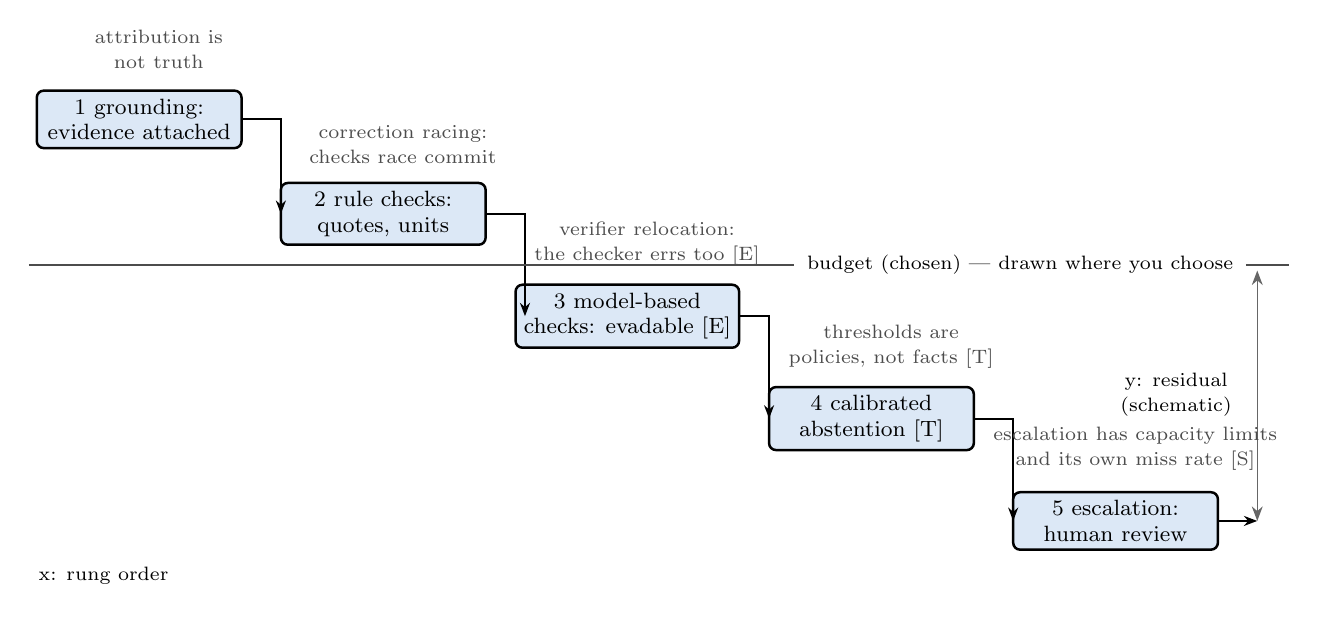
\begin{tikzpicture}[x=1mm,y=1mm]
\tikzset{
  rs/l5node/.style={rs/gModel, minimum width=26mm},
  rs/l5leak/.style={rs/gEdgeLbl, align=center, anchor=south, text=black!70},
  rs/l5lbl/.style={rs/gLegend, anchor=center, align=center},
}
% ===== five rungs on a descending stepped residual =====
\node[rs/l5node] (r1) at (14,14)  {1 grounding:\\evidence attached};
\node[rs/l5node] (r2) at (45,2)   {2 rule checks:\\quotes, units};
\node[rs/l5node] (r3) at (76,-11) {3 model-based\\checks: evadable [E]};
\node[rs/l5node] (r4) at (107,-24){4 calibrated\\abstention [T]};
\node[rs/l5node] (r5) at (138,-37){5 escalation:\\human review};
% ===== the steps: tread at each rung, riser into the next rung's west edge =====
\draw[rs/gFlow] (r1.east) -- (32,14) -- (32,2);
\draw[rs/gFlow] (r2.east) -- (63,2)  -- (63,-11);
\draw[rs/gFlow] (r3.east) -- (94,-11) -- (94,-24);
\draw[rs/gFlow] (r4.east) -- (125,-24) -- (125,-37);
\draw[rs/gFlow] (r5.east) -- (156,-37);
% ===== the chosen budget line =====
% The label is IN-LINE at the line's right end: the rule BREAKS at the label and resumes after it, so
% the text rides the budget level instead of floating above it (a floating label let the line read as
% an accidental rule through the riser). The rule still reaches x=160 so the residual bracket at
% x=156 hangs off the budget level, and the label stops at 154.2 to leave that bracket its own ink.
% Wording is a policy statement, not a measurement: the crossing point is where the operator chooses,
% not where this stack measured anything.
\node[rs/l5lbl, anchor=east] (budgetlbl) at (154.2,-4.5)
  {budget (chosen) \textemdash{} drawn where you choose};
\draw[black!70, line width=0.9pt] (0,-4.5) -- ([xshift=-1pt]budgetlbl.west);
\draw[black!70, line width=0.9pt] ([xshift=1pt]budgetlbl.east) -- (160,-4.5);
% ===== residual bracket at the last step =====
\draw[<->, >=Stealth, line width=0.5pt, draw=black!60] (156,-5.2) -- (156,-37);
\node[rs/l5lbl, anchor=east] at (154,-21) {y: residual\\(schematic)};
% ===== axis-mapping aid (both axes ordinal; see caption) =====
\node[rs/l5lbl, anchor=west] at (0,-44) {x: rung order};
% ===== named leaks, one per step =====
\node[rs/l5leak] at (16.5,20)  {attribution is\\not truth};
\node[rs/l5leak] at (47.5,8)   {correction racing:\\checks race commit};
\node[rs/l5leak] at (78.5,-5)  {verifier relocation:\\the checker errs too [E]};
\node[rs/l5leak] at (109.5,-18){thresholds are\\policies, not facts [T]};
\node[rs/l5leak] at (140.5,-31){escalation has capacity limits\\and its own miss rate [S]};
\end{tikzpicture}
}
  \caption{ Layer 5 schematic: the chosen budget line against the residual it leaves. Five rungs in cost order (x) against residual risk (y); both axes are ordinal. The residual steps down at each rung and every step leaks --- attribution is not truth, correction racing, verifier relocation [E], thresholds are policies [T], escalation capacity [S] --- and the gap between the chosen budget and the last step is bracketed as the residual. The fourth envelope item, unsound auditing, is not a rung: monitors are evadable under ordinary task pressure (\cref{sec:l5-monitoring}). No rates are encoded: step heights are deliberately uneven and the crossing point is schematic. The budget line is drawn where the operator chooses --- its placement is illustrative.}
  \label{fig:layer5-assur}
\end{figure}



\begin{figure}[t]
  \centering
  \resizebox{\linewidth}{!}{% (v2 layout notes retired 2026-10-19 — see the v3 header below.)
% figures/f4_failmatrix_draft.tex — F4 v3 (2026-10-19): displacement matrix (FM-A).
% The matrix is read as a sentence per row: a failure ARISES AT an origin layer and is CAUGHT BY
% a safeguard family. Rows are therefore sorted by origin (L0 -> L4) and the origin column is part
% of the matrix (not a marginal note), so the eye sees the argument: origins cluster at L2, and
% almost every filled cell sits in the last three columns — the layer where a failure originates is
% usually not the layer that catches it. The single amber cell is the one failure caught where it
% is caused (structured-schema error, a validity failure, x output contracts+validators).
% Cells: letter = evidence class of the anchor ([T]/[E]/[V]); dashed gray glyph = named [GAP];
% empty = family not claimed for that failure. No rates, no scores — tags only.
% label: fig:failmatrix   (fig/env + \label live in main.tex)
%
% CAPTION NOTE — items the paper must defend (state these in the caption):
%   1. the ORIGIN assignment is OUR analytic cut [J], not a measured property: hallucination /
%      ungrounded generation, retrieval miss / stale sources and perception-error propagation are
%      filed under L2 because the model conditions on a representation that carries no source
%      anchor; distribution shift under L0 because the specified task distribution is the thing
%      that moved (the one genuinely ambiguous row — assign L0 and say so); miscalibration /
%      reward hacking under L1 (objective + procedure); structured-schema error (a validity
%      failure, not a value error) and decision-model framing under L4 (contract variables).
%      Sorting by origin is a reading aid, not a claim of causal ordering;
%   2. the row reading needs ONE worked example per layer in the sec:selection prose (origin ->
%      catch -> residual). The figure asserts the pattern; the text must carry the instance;
%   3. anchors per cell are unchanged from v2: R1C4 [E] 2609.35794; R2C3 [E] 2609.33843 + Jev Bench
%      (CONTESTED direction — keep the caveat); R3C1 [E] 2609.35794, R3C3 [T] 2405.01563, R3C4
%      [GAP] human-review catch rate; R4C1 [E] 2609.35794; R5C2/R5C4 [GAP] hybrid propagation;
%      R6C3 [T] 2605.26379 + 2606.12471 + 2607.22430, R6C2/R6C4 [GAP] identifiability bridge;
%      R7C2 amber [E] 2305.13971 / 2501.10868 / 2411.15100 (validity != truth residual), R7C3 [T]
%      2607.04430; R8C2 [V] Laya TD option budget + 2610.02267 [E] failure side (30% order flip),
%      R8C4 [GAP];
%   4. amber = the ONE ledger-defended item (schema compliance is table stakes): the only cell on
%      the matrix's diagonal family, where cause and catch are the same layer;
%   5. the v2 footer is compressed into one line; no rates are claimed anywhere in the figure.
\providecommand{\figneqa}{{\fontsize{8.2}{10}\selectfont $\ne$}}
\tikzset{
  rs/gCell/.style={rounded corners=2.5pt, draw=black, line width=0.9pt, fill=white,
    minimum size=6.2mm, inner sep=0.4pt, font=\fontsize{7.6}{9.2}\selectfont\bfseries},
  rs/gCellAcc/.style={rs/gCell, fill=rsyellow!40, line width=1.2pt},
  rs/gCellGap/.style={rounded corners=2.5pt, draw=black!45, line width=0.9pt, dashed,
    fill=black!8, minimum size=6.2mm, inner sep=0.4pt,
    font=\fontsize{7.6}{9.2}\selectfont, text=black!55},
  rs/gRowLbl/.style={font=\fontsize{7.5}{9.0}\selectfont, text=black, align=right, inner sep=1pt},
  rs/gColHdr/.style={rs/gInfra, minimum width=25mm, minimum height=8mm,
    font=\fontsize{7.5}{9.0}\selectfont},
  rs/gOrig/.style={font=\fontsize{7.5}{9.0}\selectfont\bfseries, text=black!70, align=center},
}
\begin{tikzpicture}[x=1mm,y=1mm]
% ===== geometry: origin spine 0..14, four safeguard columns 14..126 (28mm pitch) =====
\draw[black!45, line width=0.5pt] (14,0) rectangle (126,-76);
\foreach \gx in {42,70,98} { \draw[black!45, line width=0.5pt] (\gx,0) -- (\gx,-76); }
\foreach \gy in {-9.5,-19,-28.5,-38,-47.5,-57,-66.5} { \draw[black!45, line width=0.5pt] (14,\gy) -- (126,\gy); }
% origin spine: one block per origin layer, no internal row rules
\draw[black!45, line width=0.5pt] (0,0) rectangle (14,-76);
\foreach \gy in {-9.5,-19,-57} { \draw[black!45, line width=0.5pt] (0,\gy) -- (14,\gy); }
\node[rs/gOrig] at (7,-4.75)  {L0};
\node[rs/gOrig] at (7,-14.25) {L1};
\node[rs/gOrig] at (7,-38)    {L2};
\node[rs/gOrig] at (7,-66.5)  {L4};
% ===== axis titles: arises at / caught by =====
\node[rs/gLegend, anchor=center, align=center] at (7,15.5) {arises\\at [J]};
\node[rs/gLegend, anchor=west] at (16,15.5) {caught by};
% ===== column headers (safeguard families) =====
\node[rs/gColHdr] at (28,9.5) {retrieval grounding};
\node[rs/gColHdr] at (56,9.5) {output contracts\\and validators};
\node[rs/gColHdr] at (84,9.5) {calibrated acceptance\\and abstention};
\node[rs/gColHdr] at (112,9.5){monitoring\\and escalation};
% ===== row labels, sorted by origin layer =====
\node[rs/gRowLbl, anchor=east] at (-3,-4.75)  {distribution shift};
\node[rs/gRowLbl, anchor=east] at (-3,-14.25) {miscalibration /\\reward hacking};
\node[rs/gRowLbl, anchor=east] at (-3,-23.75) {hallucination /\\ungrounded generation};
\node[rs/gRowLbl, anchor=east] at (-3,-33.25) {retrieval miss /\\stale sources};
\node[rs/gRowLbl, anchor=east] at (-3,-42.75) {perception-error\\propagation (hybrid)};
\node[rs/gRowLbl, anchor=east] at (-3,-52.25) {JEPA: prediction\\\figneqa\ planning};
\node[rs/gRowLbl, anchor=east] at (-3,-61.75) {structured-schema\\error (validity)};
\node[rs/gRowLbl, anchor=east] at (-3,-71.25) {decision-model\\framing sensitivity};
% ===== coverage glyphs =====
\node[rs/gCell] at (112,-4.75) {E};        % L0 x monitoring
\node[rs/gCell] at (84,-14.25) {E};        % L1 x acceptance (contested direction)
\node[rs/gCell] at (28,-23.75) {E};        % L2 hallucination x grounding
\node[rs/gCell] at (84,-23.75) {T};        % L2 hallucination x acceptance
\node[rs/gCellGap] at (112,-23.75) {$\varnothing$};
\node[rs/gCell] at (28,-33.25) {E};        % L2 retrieval miss x grounding
\node[rs/gCellGap] at (56,-42.75) {$\varnothing$};
\node[rs/gCellGap] at (112,-42.75) {$\varnothing$};
\node[rs/gCellGap] at (56,-52.25) {$\varnothing$};
\node[rs/gCell] at (84,-52.25) {T};        % L2 JEPA x acceptance
\node[rs/gCellGap] at (112,-52.25) {$\varnothing$};
\node[rs/gCellAcc] at (56,-61.75) {E};     % L4 structured-schema (validity) x contracts — caught where caused
\node[rs/gCell] at (84,-61.75) {T};        % L4 schema x acceptance
\node[rs/gCell] at (56,-71.25) {V};        % L4 framing x contracts
\node[rs/gCellGap] at (112,-71.25) {$\varnothing$};
% ===== legend: two definition lines + one footer line =====
\node[rs/gCell, minimum size=5mm, font=\fontsize{7.5}{9.0}\selectfont\bfseries] (lg1) at (2.5,-83) {E};
\node[rs/gLegend, anchor=west] at (6.5,-83) {= documented coverage of that failure; letter = the anchor's evidence class:};
\node[rs/gLegend, anchor=west] at (10,-87.2) {[T] theory-under-assumptions \textperiodcentered\ [E] independent empirical \textperiodcentered\ [V] vendor/developer-reported};
\node[rs/gCellGap, minimum size=5mm] (lg2) at (2.5,-92.6) {$\varnothing$};
\node[rs/gLegend, anchor=west] at (6.5,-92.6) {= named [GAP] in our evidence base; empty cell = family not claimed for that failure;};
\node[rs/gCellAcc, minimum size=5mm, font=\fontsize{7.5}{9.0}\selectfont\bfseries] (lg3) at (2.5,-97.4) {E};
\node[rs/gLegend, anchor=west] at (6.5,-97.4) {= ledger-defended item: schema compliance is table stakes --- validity \figneqa\ truth, three [E] anchors;};
\node[rs/gLegend, anchor=west] at (10,-101.6) {the one cell where the catch sits in the same layer family as the cause};
\node[rs/gLegend, anchor=west] at (0,-106.5) {unmeasured rows: hybrid error-propagation; identifiability to decision quality ---};
\node[rs/gLegend, anchor=west] at (10,-110.8) {every glyph is anchored in the claim ledger; no coverage rates are claimed};
\end{tikzpicture}
}
  \caption{ Failure modes sorted by the layer where they arise, against the safeguard families that catch them. Read each row as a sentence --- originates at Lx, caught by --- and the argument appears: origins cluster at L2 (representation) while filled cells cluster in the last three columns, so the layer where a failure originates is usually not the layer that catches it. The amber cell is the single same-layer catch: structured-schema (validity) error caught by output contracts and validators --- and it closes only the validity half; the value error survives (validity $\ne$ truth). Origin assignment is our analytic cut [J] --- distribution shift is the ambiguous row, filed at L0 and stated as such. Glyphs: E/T/V = documented coverage of that failure and the evidence class of the anchor; $\varnothing$ = named [GAP]; empty = family not claimed. No coverage rates are claimed.}
  \label{fig:failmatrix}
\end{figure}

\section{Case Studies}\label{sec:cases}
% ===== P4: Section 9 case-study cards (my prose from cards/case-evidence-packs.md) =====

Seven recurring reliable-AI engineering settings are our case studies. Each is an \emph{instance}
of the stack of \cref{sec:stack}, and each is documentation-anchored
rather than drawn from a measured population of deployments. What they demonstrate, then, is
the framework fitting together, and the seven-row comparison, with Case~6 as the null, tests
that.
Per our protocol (\cref{sec:protocol}), every claim a card rests on is carried in the ledger
with its class. Cards mark the class where it changes the reading, and \cref{tab:crosscase}
gives the per-case summary.
\cref{fig:case-rag,fig:case-decision,fig:case-hybrid,fig:case-jepa,fig:case-classifier,fig:case-forms,fig:case-diffusion}
give the seven architecture sketches; each case's sketch follows its prose.

\subsection{Case 1: Retrieval-augmented LLM assistant}
\label{sec:case-rag}
The dominant deployment class is an open-ended knowledge task on an autoregressive objective,
with provenance deliberately externalized to a retrieval index whose shape --- flat, graph, or
episodic log --- is itself a selection with measured consequences (\cref{sec:l5-grounding}).
Case~1's closed corpus is the instance where flat is the
right choice; we keep it and decline the alternative. The reliability literature is
dense but disorganized: the trustworthy-RAG surveys collect reliability as per-dimension
technique checklists ~\cite{id250206872,id240910102}, and the hallucination surveys map a
single failure mode across a lifecycle rather than a design-objective
stack~\cite{id230901219,id251006265}. On the positive side, a live empirical line teaches the
model to abstain when retrieved evidence cannot support a response~\cite{id260935794} [E], and
conformal abstention supplies an assumption-bound procedure for deciding when to
refuse~\cite{id240501563} [T]. Self-consistency remains the incumbent model-level
mitigation~\cite{id220311171}, with no dedicated survey (a named gap in our ledger).
\emph{Inherited failure mode:} hallucination is intrinsic to the objective; compositional
effects of chaining retrieval with conformal and self-consistency layers are unmeasured in our
evidence, as is human reviewers' catch rate. \cref{fig:case-rag} marks both gaps as dashed
wiring. Remove the L4 contract --- citations as structured metadata --- and the grounding gate
has nothing to check; remove L5 and the contract certifies form only. The gate catches citation
mismatch; post-rationalization sits outside it, and \cref{sec:l5-grounding} prices that gap at a
measured miss rate. The instance is reliable only as that pair.


\begin{figure}[h!]
  \centering
  \resizebox{\linewidth}{!}{% figures/f_case_rag.tex — Case-study sketch (pack 1): RAG-LLM assistant. Grammar: figures/style_v2_tokens.tex (v8 token grammar).
% Roles: task / answer+citations = rs/gData (payload); embed query, generalist LLM, validators =
%   rs/gModel; external index = rs/gStore (drum = store, not a step); review escalation = rs/gInfra
%   (service); retrieval container = rs/gPanelFill/rs/gPanelEdge pair (tint underlay + border/title).
% Chain: task -> retrieval (embed query -> external index) -> generalist LLM -> free-form answer
%   -> L5 mitigation chain: grounding gate -> validators -> review escalation.
% Accent: the ONE yellow = the item the evidence ledger defends, the retrieval-grounding abstention
%   gate [E]; dashed edges = contested mitigation-composition effects (joint effect unmeasured [GAP]).
% label: fig:case-rag   (figure env + \label live in main.tex; case-studies slot, owner wires)
%
% CAPTION NOTE — items the paper must defend (state these in the caption):
%   1. [E] grounding gate = ledger L5 anchor 2609.35794 (abstain when retrieved evidence cannot
%      support a response); conformal abstention threshold procedure [T] 2405.01563 is assumption-bound;
%   2. dashed edges = mitigation composition (retrieval + conformal + self-consistency):
%      joint effect unmeasured in our evidence [GAP]; no system-level acceptance test for an
%      assembled RAG assistant exists in our anchors [GAP];
%   3. human review is an L5 control with no quantified error-catch rate [GAP];
%   4. L4 stays a free-form text contract (no closure); schema enforcement lives in the forms case.
% Fonts >= 7.5pt; math glyphs measure ~0.92x nominal (CMSY/CMR quirk) so symbols use 8.2pt.
\providecommand{\figplus}{{\fontsize{8.2}{10}\selectfont $+$}}
\providecommand{\figsep}{{\fontsize{8.2}{10}\selectfont $|$}}
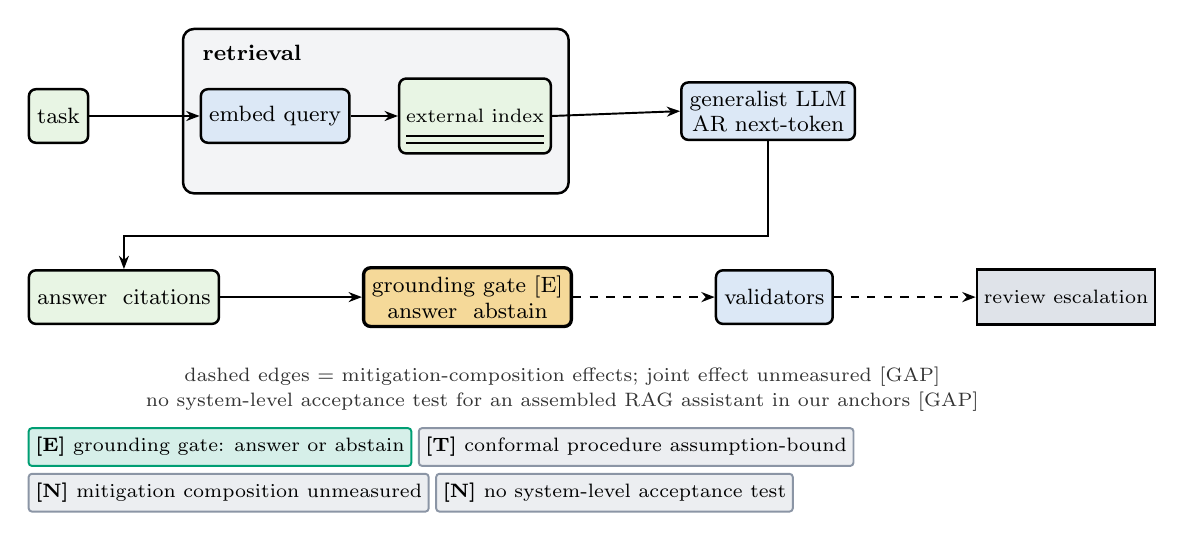
\begin{tikzpicture}
\pgfdeclarelayer{rsbg}\pgfsetlayers{rsbg,main}  % panel tints render UNDER their tiles
% ===== row 1: task -> retrieval (embed query -> external index) -> generalist LLM =====
\node[rs/gData] (in1) {task};
\node[rs/gModel, right=14mm of in1] (r1) {embed query};
\node[rs/gStore, right=6mm of r1] (r2) {external index};
\coordinate (padtop) at ([yshift=3.5pt]r2.north);  % opens the title band so the header clears the cylinder top
\begin{pgfonlayer}{rsbg}
  \node[rs/gPanelFill, fit=(r1)(r2)(padtop)] {};
\end{pgfonlayer}
\node[rs/gPanelEdge, fit=(r1)(r2)(padtop),
      label={[rs/gPanelTitle, xshift=4pt, yshift=-9pt]north west:retrieval}] (ret) {};
\node[rs/gModel, right=14mm of ret.east] (llm) {generalist LLM\\AR next-token};
% ===== row 2: answer -> grounding gate (accent) -> validators -> review escalation =====
\node[rs/gData, anchor=north west] (ans) at ([yshift=-23mm]in1.north west) {answer \figplus\ citations};
\node[rs/gAccent, right=18mm of ans] (gate) {grounding gate [E]\\answer \figsep\ abstain};
\node[rs/gModel, right=18mm of gate] (val) {validators};
\node[rs/gInfra, right=18mm of val] (esc) {review escalation};
% ===== edges: solid = documented wiring; dashed = contested mitigation composition [GAP] =====
\draw[rs/gFlow] (in1.east) -- (r1.west);   % through the container wall to the content: no wall-to-box gutter
\draw[rs/gFlow] (r1.east) -- (r2.west);
\draw[rs/gFlow] (r2.east) -- (llm.west);   % leaves the content, crossing the container wall
\draw[rs/gFlow] (llm.south) -- ++(0,-12mm) -| (ans.north);   % pipe wraps to the L5 row
\draw[rs/gFlow] (ans.east) -- (gate.west);
\draw[rs/gFlowD] (gate.east) -- (val.west);
\draw[rs/gFlowD] (val.east) -- (esc.west);
% ===== foot =====
\coordinate (mid) at ($(in1.center)!0.5!(esc.center)$);
\node[rs/gFoot] at ([yshift=-8mm]mid |- esc.south) {dashed edges = mitigation-composition effects; joint effect unmeasured [GAP]\\no system-level acceptance test for an assembled RAG assistant in our anchors [GAP]};
% --- evidence ribbon (P2): segments are claims already carried above; tag = the claim's class.
\rsRibbonBase{-3.4mm}
\rsRibbonRow{0mm}
\rsRibSeg{rsVerified}{\textbf{[E]} grounding gate: answer or abstain}
\rsRibSeg{rsNoClaim}{\textbf{[T]} conformal procedure assumption-bound}
\rsRibbonRow{-5.8mm}
\rsRibSeg{rsNoClaim}{\textbf{[N]} mitigation composition unmeasured}
\rsRibSeg{rsNoClaim}{\textbf{[N]} no system-level acceptance test}
\end{tikzpicture}
}
  \caption{Case 1: retrieval-augmented assistant. Accent = ledger-admissible grounding gate ($[E]$ recovery-abstention line + assumption-bound conformal procedure $[T]$); dashed = mitigation composition and system-level-acceptance coverage, both named gaps; human review remains un-quantifiable [GAP]. Glyph: the two thin rules in the store box = stored records; the external index is a data store that is retrieved from, outside the processing path.}
  \label{fig:case-rag}
\end{figure}

\subsection{Case 2: Decision-model serving}
\label{sec:case-decision}
This case exercises every layer. At L0, bounded decisions over closed option sets; at L4 the
contract is the typed primitives \texttt{choice}/\texttt{score}/\texttt{noul} (target
vocabulary of the Laya-class systems), returned from a single forward pass of a non-generative
model \cite{rauk2026jevbenchmark,id260934024,id261018529}. The boundary-setting evaluation
literature describes the contract class independently of the vendor
~\cite{id261002076,id261013675,id261019811}: multimodal decision models, per-dataset diagnostic
QA gating, calibration metrics. Training aligns with proper scoring rules (log + spherical +
ranked-probability score) of the Laya-class recipe; we anchor the recipe to the vendor's
shipped documentation \evvendor{}.\footnote{The vendor-named training scheme shares an
acronym with an unrelated older method (``RLCD''); we cite the vendor's usage only, so the
label does not ride on the older literature.} The vendor reports threshold-as-policy (``a
threshold is a policy you choose from measured accuracy \ldots on your data, not a property of
the model''), our L5 epigraph; but the family's reliability claims require the
contested-direction caveat: \evindep{the shipped Typed-Decisions checkpoint was independently
measured \emph{under}-confident (signed gap $-0.214$)}, the opposite of the card's framing, and the
direction decides which way a confidence-gated cascade fails~\cite{id260933843}. The deployed
gate --- thresholds frozen before evaluation --- beats random escalation on both reported
tracks, but \evindep{misses its 10\% accepted-error target on each track} \cite{id260933843}. The headline \evindep{30\% of answers flip when option order
reverses, and accuracy drops sharply at 50 similar candidates~\cite{id261002267}}. Third-party entrants
now contest benchmark-leader margins with KL/Brier metrics, and those margins carry
labelling-teacher saturation caveats~\cite{id261020778}. Because a typed decision acts without
a human reader in the loop, the verdict is the attack surface: black-box attacks flip the
verdicts of verified-reward models without touching their weights~\cite{id260931142}, and
decision models already serve inside autonomous penetration-testing
harnesses~\cite{id260928940}. A 2026 red team of a due-diligence deployment \evindep{broke 25 of 27 Jev
configurations at roughly \$0.50 per break, its strongest attacker succeeding on 9 of
9}~\cite{checkpoint2026jevredteam}; on that record the typed output did not harden the contract \evjudge{}.

\emph{What this instance leaves unmeasured:} no anchor evaluates a fully deployed decision-model system end-to-end (harness + gate + escalation); the joint effect of the documented fixes (temperature refit, option shuffling, shortlist workaround) is unmeasured in our evidence.

\begin{figure}[h!]
  \centering
  \resizebox{\linewidth}{!}{% figures/f_case_decision.tex — Case-study sketch (pack 2): decision-model system (Laya/Jev-class).
% Grammar: figures/style_v2_tokens.tex (v8 token grammar).
% Roles: state+question / typed decision / act / risk budget = rs/gData; single-pass engine =
%   rs/gModel; calibrated acceptance = rs/gAccent (the ONE ledger-defended item); escalate / defer =
%   rs/gInfra (service). The reliability inset is ink/gray only (no role fill): its means and the
%   gate miss are [E] measurements; the vermillion dashed leader marks the [C] direction claim
%   (which way a confidence-gated cascade fails), not the measurement.
% Chain: state + typed question -> single-pass decision engine -> typed decision -> calibrated
%   acceptance (threshold-as-policy) -> act / escalate. Risk budget (L0) sets the acceptance
%   threshold (vertical edge from above). The inset hangs over act on the [C] leader.
% label: fig:case-decision   (figure env + \label live in main.tex; case-studies slot, owner wires)
%
% CAPTION NOTE — items the paper must defend (state these in the caption):
%   1. [E] typed contract 2609.37647: no generation; choice/score/noul over a closed option set
%      (spelling 'noul' is per vendor docs — do not correct to 'null'; Jev only — that benchmark
%      evaluated no Laya checkpoint);
%   2. [V] threshold-as-policy + RLCD proper-scoring-rule recipe (Laya repo); "RLCD" is never
%      expanded in-repo — do not conflate with the unrelated 2307.12950;
%   3. [E] contested calibration direction: shipped TD checkpoint is uniformly UNDER-confident,
%      signed gap -0.214 (2609.33843), contradicting the card's over-confidence framing; the
%      direction decides which way a confidence-gated cascade fails; the frozen gate misses its
%      10% accepted-set error target on both tracks [E] — cite per checkpoint, not per family;
%   4. [E] option-set instability 2610.02267: 30% option-order flip + 31% at 50 candidates
%      (vs Jev 98% on unique-tool items); interface generality: fine-tuned AR LLMs + multimodal
%      (2610.02076 / 2610.13675);
%   5. [GAP] no end-to-end deployed decision-system eval (harness + gate + escalation); joint
%      effect of the documented fixes unmeasured.
% Fonts >= 7.5pt; math glyphs measure ~0.92x nominal (CMSY/CMR quirk) so symbols use 8.2pt.
\providecommand{\figplus}{{\fontsize{8.2}{10}\selectfont $+$}}
\providecommand{\figsep}{{\fontsize{8.2}{10}\selectfont $|$}}
\providecommand{\figeq}{{\fontsize{8.2}{10}\selectfont $=$}}
\providecommand{\figminus}{{\fontsize{8.2}{10}\selectfont $-$}}
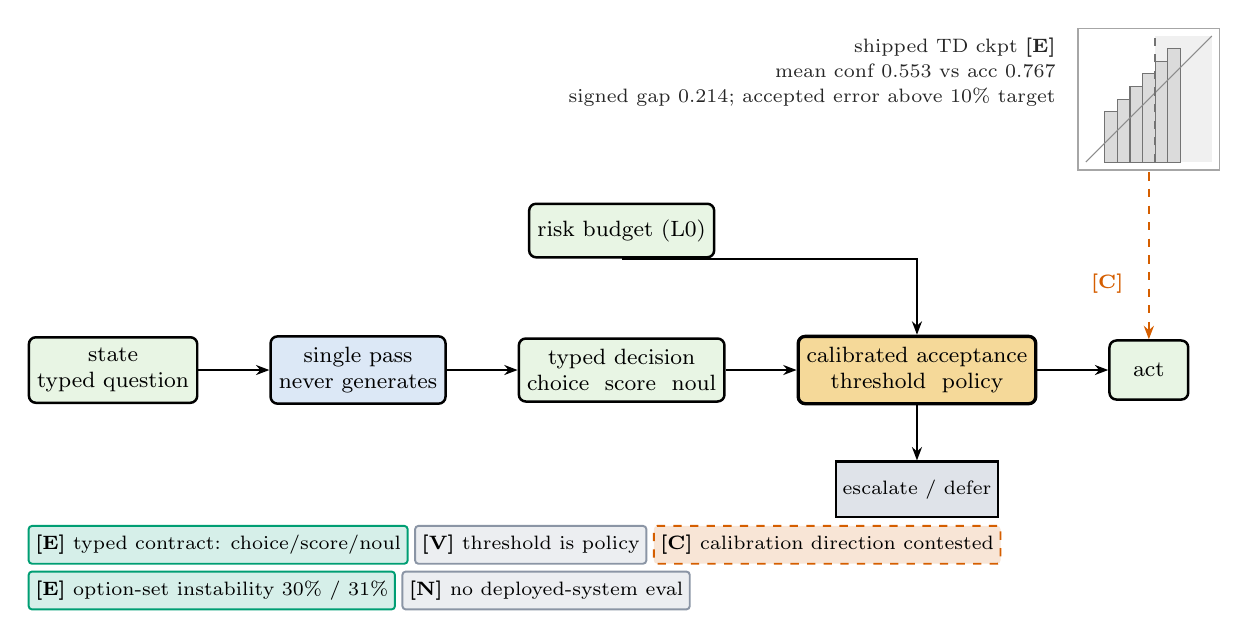
\begin{tikzpicture}
% ===== inference chain =====
\node[rs/gData, inner ysep=4pt] (in1) {state \figplus\\typed question};
\node[rs/gModel, right=9mm of in1, inner ysep=4pt] (eng) {single pass\\never generates};
\node[rs/gData, right=9mm of eng, inner ysep=4pt] (tif) {typed decision\\choice \figsep\ score \figsep\ noul};
\node[rs/gAccent, right=9mm of tif, inner ysep=4pt] (acc) {calibrated acceptance\\threshold \figeq\ policy};
\node[rs/gData, right=9mm of acc, minimum width=10mm, minimum height=7.5mm] (act) {act};
\node[rs/gInfra, below=7mm of acc] (esc) {escalate / defer};
% ===== L0 risk budget (left of the acceptance gate, sets the threshold) =====
\node[rs/gData, above=10mm of tif] (rb) {risk budget (L0)};
% ===== reliability inset (replaces the old contested tile): the anchor's own reliability
% diagram, redrawn. x = confidence bin, y = accuracy; the diagonal is perfect calibration and
% every bar sits a near-constant offset ABOVE it (uniform under-confidence). The dashed rule is
% the policy cut, the pale band right of it the accepted region. No axis ticks/numbers (they
% would publish sub-floor at 18mm); bin spacing is schematic, the two means + the gate miss are
% the measured anchors. The [C] direction claim survives as the vermillion dashed leader + tag.
\coordinate (rib) at ($(act.north)+(-9mm,21.5mm)$);
\begin{scope}[shift={(rib)}, x=1mm, y=1mm]
\fill[white] (0,0) rectangle (18,18);                                % opaque backing for the inset
\fill[black!6] (9.8,1) rectangle (17,17);                            % accepted region (x >= cut)
\foreach \i/\c/\a in {0/0.20/0.40, 1/0.30/0.50, 2/0.40/0.60,
                     3/0.50/0.70, 4/0.60/0.80, 5/0.70/0.90} {
  \pgfmathsetmacro{\bx}{1+16*\c-0.8}
  \pgfmathsetmacro{\bh}{16*\a}
  \fill[black!14] (\bx,1) rectangle ++(1.6,\bh);                     % one occupied confidence bin
  \draw[black!55, line width=0.4pt] (\bx,1) rectangle ++(1.6,\bh);
}
\draw[black!45, line width=0.4pt] (1,1) -- (17,17);                  % perfect calibration (over the bars)
\draw[black!55, line width=0.5pt, dashed] (9.8,1) -- ++(0,16);       % threshold = policy, in a bin gap
\draw[draw=black!35, line width=0.4pt] (0,0) rectangle (18,18);
\node[anchor=north east, align=right, font=\fontsize{7.5}{9.0}\selectfont, text=black!85]
  at (-1.6,18)
  {shipped TD ckpt \textbf{[E]}\\mean conf 0.553 vs acc 0.767\\
   signed gap \figminus 0.214; accepted error above 10\% target};
\end{scope}
% ===== edges =====
\draw[rs/gFlow] (in1.east) -- (eng.west);
\draw[rs/gFlow] (eng.east) -- (tif.west);
\draw[rs/gFlow] (tif.east) -- (acc.west);
\draw[rs/gFlow] (acc.east) -- (act.west);
\draw[rs/gFlow] (acc.south) -- (esc.north);
\draw[rs/gFlow] (rb.south) -| (acc.north);   % elbow: fills the upper-left band instead of a lone tall riser
% [C] direction: the offset is measured [E]; which way a confidence-gated cascade fails is contested [C]
\draw[rsContested, dashed, line width=0.9pt, -{Stealth[length=1.7mm]}]
  ($(act.north)+(0,21.2mm)$) -- (act.north);
\node[rs/gTiny, anchor=east, text=rsContested] at ($(act.north)+(-2mm,7mm)$) {\textbf{[C]}};
% --- evidence ribbon (P2): segments are claims already carried above; tag = the claim's class.
\rsRibbonBase{-3.4mm}
\rsRibbonRow{0mm}
\rsRibSeg{rsVerified}{\textbf{[E]} typed contract: choice/score/noul}
\rsRibSeg{rsNoClaim}{\textbf{[V]} threshold is policy}
\rsRibSeg[dashed]{rsContested}{\textbf{[C]} calibration direction contested}
\rsRibbonRow{-5.8mm}
\rsRibSeg{rsVerified}{\textbf{[E]} option-set instability 30\% / 31\%}
\rsRibSeg{rsNoClaim}{\textbf{[N]} no deployed-system eval}
\end{tikzpicture}
}
  \caption{ Case 2: decision-model serving. Accent = calibrated acceptance as threshold-as-policy (locked to $[V]$ vendor docs and $[E]$ independent benchmarking). Inset: the shipped TD checkpoint's reliability diagram (\cite{id260933843}) --- the bars are the confidence bins, bar height is accuracy in that bin, and the diagonal is perfect calibration, so bars above it are under-confidence; the dashed rule is the policy cut and the shaded band is the accepted set (bin spacing schematic); measured mean confidence 0.553 vs accuracy 0.767 (signed gap $-0.214$), and the accepted set misses its 10\% error target $[E]$. The vermillion dashed leader marks the $[C]$ claim: the card frames the cascade as failing toward over-confidence, while the independent measurement finds the shipped checkpoint under-confident --- the direction is contradicted (anchor named); the measurement stands. End-to-end-system evidence remains a named gap.}
  \label{fig:case-decision}
\end{figure}

\subsection{Case 3: Hybrid specialist (Interfaze-class)}
\label{sec:case-hybrid}
This case instantiates an architecture class: task-specific DNNs/CNNs fused into a transformer
decoder through a shared embedding space~\cite{interfaze2026} (\cref{fig:case-hybrid}). Its
value is representational: the specialist channel returns structured fields (boxes,
coordinates, confidence values) that the stack can check, and the fusion layer absorbs
interaction errors when a specialist meets inputs outside its training distribution.
Multi-expert adapters have precedents in the literature~\cite{id230317580,id240509818}, and the
distinction between intra- and system-level routing matters here too~\cite{id240706204}. The
metadata stream is only verifiable because the specialists return typed fields; a generalist
producing the same fields as text would leave the fusion layer nothing to check. Our verdict
stays restrained: the case's value is that check. \emph{Inherited failure:} cross-component
error propagation is known to be a leading reliability cost in per-component
pipelines~\cite{mdpi2026arlm}; all evaluation evidence is vendor-class, and no independent
propagation or end-to-end comparison anchor exists in our evidence set.

\begin{figure}[h!]
  \centering
  \resizebox{\linewidth}{!}{% figures/f_case_hybrid_v8.tex — case study 3 (Interfaze-class hybrid specialist): FLAGSHIP architecture panel, v8.
% Style: figures/style_v2_tokens.tex ONLY (semantic role tokens; rs/g* family). Wired into main.tex (case-3 figure env).
%
% SPEC (gate 1, takeaway-first):
%   ONE takeaway: this class of system separates perception, reasoning, generation and infra into
%   nested containers with distinct roles, and the reliability-critical path runs through the
%   validation layer. Components (from the verified case-3 instance, interfaze2026):
%   prompt input -> preprocessor (cache lane) -> core block (DNN/CNN adapters stacked over a
%   transformer core, fused via the shared embedding space) -> decoder stage (task decoders,
%   reasoning, fallback) -> validation layer -> outputs (free text + structured output);
%   infra foundation lane alongside (vector DB, code sandbox, web index, browser engine, GPU scale).
%   Encoding: shape = role (rounded model / cylinder store / octagon control / sharp infra /
%   tinted panel); dashed = wiring the vendor description leaves undocumented (validators,
%   monitors, escalation); long-dash = reliability-critical path; yellow = the ONE item the
%   evidence ledger defends ([V] architecture claim 2602.04101: the native fusion).
%   Caption carries: vendor-only evidence class, no independent propagation measurement,
%   dashes = undocumented wiring. Figure env + \label (fig:case-hybrid-v8) live in main.tex.
%
% LAYOUT NOTE: the three top containers are TOP-ALIGNED and the spine arrows sit on one
% horizontal line (pin.center = adapters.center = decoders.center); yshift values below are
% render-verified so the tile-row centers coincide (re-verify if tile sizes change).
% v8fix wave: the infra foundation lane spans the FULL pipeline width (panel edges flush with
% fpre.west / ostruct.east; 5 tiles at uniform 64pt width + 31.34pt gap), and its two dashed
% attachments are SHORT VERTICAL stubs dropped at the fcore/fdec centre x (no near-horizontal
% diagonals). The core->decoder Z-bend enters the decoder stage at the task-decoders TILE
% boundary (was: container border).
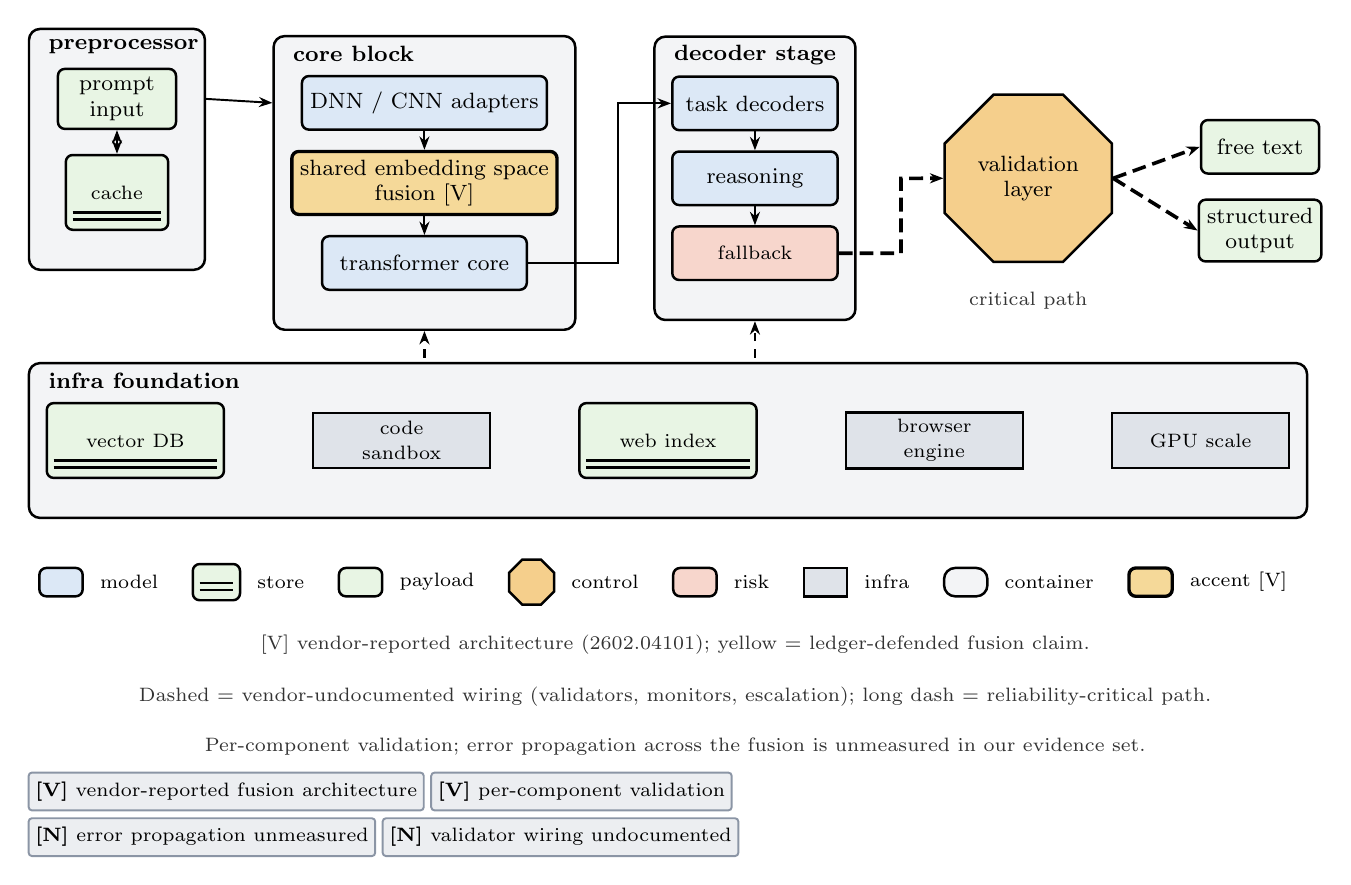
\begin{tikzpicture}
  \pgfdeclarelayer{rsbg}\pgfsetlayers{rsbg,main}  % panel tints render UNDER their tiles
  % ===== preprocessor panel: REAL containment (input + cache lane) =====
  \node[rs/gData, minimum width=15mm] (pin) {prompt\\input};
  \node[rs/gStore, below=3mm of pin] (pcache) {cache};
  \begin{pgfonlayer}{rsbg}
    \node[rs/gPanelFill, inner xsep=10pt, fit=(pin)(pcache)] {};
  \end{pgfonlayer}
  \node[rs/gPanelEdge, inner xsep=10pt, fit=(pin)(pcache),
        label={[rs/gPanelTitle, xshift=4pt, yshift=-7pt]north west:preprocessor}] (fpre) {};
  % ===== core block panel: adapters stacked over transformer core, fused via shared embedding =====
  % yshift: puts adapters.center at pin.center -> top-aligned containers, horizontal spine line
  \node[rs/gModel, minimum width=26mm, right=12mm of fpre.east, yshift=16.8pt] (adapters) {DNN / CNN adapters};
  \node[rs/gAccent, minimum width=30mm, below=2.4mm of adapters] (fusion) {shared embedding space\\fusion [V]};
  \node[rs/gModel, minimum width=26mm, below=2.4mm of fusion] (tcore) {transformer core};
  \begin{pgfonlayer}{rsbg}
    \node[rs/gPanelFill, fit=(adapters)(fusion)(tcore)] {};
  \end{pgfonlayer}
  \node[rs/gPanelEdge, fit=(adapters)(fusion)(tcore),
        label={[rs/gPanelTitle, xshift=4pt, yshift=-7pt]north west:core block}] (fcore) {};
  % ===== decoder stage panel: task decoders + reasoning + fallback (risk role) =====
  % yshift: puts decoders.center on the same spine line (render-verified)
  \node[rs/gModel, minimum width=21mm, right=12mm of fcore.east, yshift=28.75pt] (decoders) {task decoders};
  \node[rs/gModel, minimum width=21mm, below=2.4mm of decoders] (reasoning) {reasoning};
  \node[rs/gRisk, minimum width=21mm, below=2.4mm of reasoning] (fallback) {fallback};
  \begin{pgfonlayer}{rsbg}
    \node[rs/gPanelFill, fit=(decoders)(reasoning)(fallback)] {};
  \end{pgfonlayer}
  \node[rs/gPanelEdge, fit=(decoders)(reasoning)(fallback),
        label={[rs/gPanelTitle, xshift=4pt, yshift=-7pt]north west:decoder stage}] (fdec) {};
  % ===== validation layer: the ONE control gate (octagon, amber) =====
  \node[rs/gControl, minimum width=23mm, right=11mm of fdec.east] (val) {validation\\layer};
  % ===== output pathway: free text + structured output =====
  \node[rs/gData, minimum width=15mm, right=11mm of val.east, yshift=4mm] (ofree) {free text};
  \node[rs/gData, minimum width=15mm, below=3mm of ofree] (ostruct) {structured\\output};
  % ===== infra foundation lane: stores (cylinders) + services (sharp rectangles) =====
  % full-width foundation: 5 tiles x 64pt + 4 x 31.82pt gaps = 447.28pt span; xshift 6.42pt puts
  % the panel's west edge flush with fpre.west (inner xsep 6pt + half stroke), east flush with
  % ostruct.east (render-verified; re-solve the gap if tile widths change)
  \node[rs/gStore, minimum width=64pt, anchor=north west] (iv) at ([yshift=-9mm, xshift=6.42pt]fcore.south west -| fpre.west) {vector DB};
  \node[rs/gInfra, minimum width=64pt, right=31.34pt of iv] (is1) {code\\sandbox};
  \node[rs/gStore, minimum width=64pt, right=31.34pt of is1] (iw) {web index};
  \node[rs/gInfra, minimum width=64pt, right=31.34pt of iw] (ib) {browser\\engine};
  \node[rs/gInfra, minimum width=64pt, right=31.34pt of ib] (ig) {GPU scale};
  \begin{pgfonlayer}{rsbg}
    \node[rs/gPanelFill, fit=(iv)(is1)(iw)(ib)(ig)] {};
  \end{pgfonlayer}
  \node[rs/gPanelEdge, fit=(iv)(is1)(iw)(ib)(ig),
        label={[rs/gPanelTitle, xshift=4pt, yshift=-7pt]north west:infra foundation}] (finf) {};
  % ===== edges: solid = documented wiring; dashed = vendor-undocumented; long heavy dash = critical path =====
  \draw[rs/gFlowDB] (pcache.north) -- (pin.south);                          % cache lane (undocumented, read/write)
  \draw[rs/gFlow]  (fpre.east |- pin.center) -- (fcore.west |- adapters.center);   % horizontal spine
  \draw[rs/gFlow]  (adapters.south) -- (fusion.north);                     % encode -> fuse
  \draw[rs/gFlow]  (fusion.south) -- (tcore.north);                        % fuse -> decode
  % Z-bend: exits at the transformer-core row (final internal stage), enters ON the top decode tile
  \draw[rs/gFlow] (tcore.east) -- ([xshift=15pt]fcore.east |- tcore.center)
                  -- ([xshift=15pt]fcore.east |- decoders.center) -- (decoders.west);
  \draw[rs/gFlow]  (decoders.south) -- (reasoning.north);
  \draw[rs/gFlow]  (reasoning.south) -- (fallback.north);
  % Z-bend: exits at the fallback row (failure path), turns into the validation gate's west side
  \draw[rs/gFlowCrit] (fallback.east) -- ([xshift=16pt]fdec.east |- fallback.center)
                  -- ([xshift=16pt]fdec.east |- val.center) -- (val.west);
  \draw[rs/gFlowCrit] (val.east) -- (ofree.west);
  \draw[rs/gFlowCrit] (val.east) -- (ostruct.west);
  % infra attachment stubs (undocumented): dash phase 4.5pt keeps the first dash clear of the
  % arrowhead, so each 12-15pt stub still reads dashed rather than head-heavy
  \draw[rs/gFlowD, dash phase=4.5pt] (fcore.south |- finf.north) -- (fcore.south);   % infra attachment (undocumented); vertical stub
  \draw[rs/gFlowD, dash phase=4.5pt] (fdec.south |- finf.north) -- (fdec.south);     % infra attachment (undocumented); vertical stub
  \node[rs/gEdgeLbl, below=3.2mm of val] {critical path};
  % ===== legend: role words per symbol (redundant encoding; readable in grayscale) =====
  \coordinate (figmid) at ($(fpre.west)!0.5!(ostruct.east)$);
  \coordinate (legy) at ([yshift=-8mm]figmid |- finf.south);
  \node[rs/gModel, minimum width=5.5mm, minimum height=3.6mm, inner sep=0.5pt] (lg1) at ([xshift=-78mm]legy) {};
  \node[rs/gLegend, right=0.8mm of lg1] (lg1t) {model};
  \node[rs/gStore, minimum width=6mm, minimum height=4.6mm, inner sep=0.5pt, right=3mm of lg1t] (lg2) {};
  \node[rs/gLegend, right=0.8mm of lg2] (lg2t) {store};
  \node[rs/gData, minimum width=5.5mm, minimum height=3.6mm, inner sep=0.5pt, right=3mm of lg2t] (lg3) {};
  \node[rs/gLegend, right=0.8mm of lg3] (lg3t) {payload};
  \node[rs/gControl, minimum width=6.2mm, inner sep=0.5pt, right=3mm of lg3t] (lg4) {};
  \node[rs/gLegend, right=0.8mm of lg4] (lg4t) {control};
  \node[rs/gRisk, minimum width=5.5mm, minimum height=3.6mm, inner sep=0.5pt, right=3mm of lg4t] (lg5) {};
  \node[rs/gLegend, right=0.8mm of lg5] (lg5t) {risk};
  \node[rs/gInfra, minimum width=5.5mm, minimum height=3.6mm, inner sep=0.5pt, right=3mm of lg5t] (lg6) {};
  \node[rs/gLegend, right=0.8mm of lg6] (lg6t) {infra};
  \node[rs/gPanelEdge, fill=rsPanelTint, minimum width=5.5mm, minimum height=3.6mm, inner xsep=0.5pt, inner ysep=0.5pt, right=3mm of lg6t] (lg7) {};
  \node[rs/gLegend, right=0.8mm of lg7] (lg7t) {container};
  \node[rs/gAccent, minimum width=5.5mm, minimum height=3.6mm, inner sep=0.5pt, right=3mm of lg7t] (lg8) {};
  \node[rs/gLegend, right=0.8mm of lg8] (lg8t) {accent [V]};
  % ===== footnotes: evidence class + dashed semantics (caveats carried, not dropped) =====
  \node[rs/gFoot, anchor=north] (f1) at ([yshift=-5.5mm]legy) {[V] vendor-reported architecture (2602.04101); yellow = ledger-defended fusion claim.};
  \node[rs/gFoot, below=1.6mm of f1] (f2) {Dashed = vendor-undocumented wiring (validators, monitors, escalation); long dash = reliability-critical path.};
  \node[rs/gFoot, below=1.6mm of f2] (f3) {Per-component validation; error propagation across the fusion is unmeasured in our evidence set.};
  % --- evidence ribbon (P2): segments are claims already carried above; tag = the claim's class.
  \rsRibbonBase{-3.4mm}
  \rsRibbonRow{0mm}
  \rsRibSeg{rsNoClaim}{\textbf{[V]} vendor-reported fusion architecture}
  \rsRibSeg{rsNoClaim}{\textbf{[V]} per-component validation}
  \rsRibbonRow{-5.8mm}
  \rsRibSeg{rsNoClaim}{\textbf{[N]} error propagation unmeasured}
  \rsRibSeg{rsNoClaim}{\textbf{[N]} validator wiring undocumented}
\end{tikzpicture}
}
  \caption{Case 3: hybrid specialist architecture, Interfaze-class $[V]$ (vendor reconstruction; dashed = vendor-undocumented; box with record rules = data store, octagon = control/validation, red = fallback risk). The validation layer is the reliability-critical path.}
  \label{fig:case-hybrid}
\end{figure}

\subsection{Case 4: JEPA world-model planner}
\label{sec:case-jepa}
This case aims at a conception of reliability that generative objectives cannot reach:
latent-predictive training \cite{id230108243}, whose planning value is conditional on
identifiability theory~\cite{klindt2026lejepa,identifiability2026,id260612471}. The
identifiability trio supplies only assumption-bound performance
guarantees~\cite{klindt2026lejepa,identifiability2026}; the transfer-to-language paradox
supplies our honest counterpoint (\cref{sec:l2-jepa}). \emph{Inherited failure:} a systematic
evaluation awaiting our full-text read is carried as $[W]$: the source is cited for a
planning-horizon cap and a success-rate fall at 20-step horizons, but its full-text check is
incomplete, so those quantities are \emph{not verified} (n/v) here and we do not use them.
Text-modality stability remains contested elsewhere in our ledger~\cite{id260723531}
\evindep{}~\textsf{[C]}.
\cref{fig:case-jepa} marks the
identifiability block as the condition the system must pay for.

\begin{figure}[h!]
  \centering
  \resizebox{\linewidth}{!}{% figures/f_case_jepa.tex — Case-study sketch (pack 4): JEPA world-model + planner (control tasks).
% Grammar: figures/style_v2_tokens.tex (v8 token grammar).
% Roles: observation / action = rs/gData; encoder, predictor, latent state, planner = rs/gModel;
%   identifiability conditions = rs/gAccent (the ONE ledger-defended item, [T]); planning-cap note =
%   rs/gRisk (failure-direction caveat; dashed = claim to defend).
% Chain: observation -> shared encoder -> latent predictor (squared-error, embedding space) ->
%   latent state (the world model) -> planner (MPC/CEM over imagined rollouts) -> action.
% Accent: the item the evidence ledger defends is identifiability conditions [T] — assumption-bound,
%   not an [E] guarantee. Dashed wires = claims-to-defend: identifiability -> latent state;
%   planning-cap note -> planner. The planning-cap numbers (5-step vs 16-53-step tasks) stay in the
%   CAPTION NOTE only — not in the figure.
% Notation note: the old "$z$" glyph is dropped from the latent-state label (semantics unchanged:
%   "the world model" carries it); math symbols ride the 8.2pt commands.
% label: fig:case-jepa   (figure env + \label live in main.tex; case-studies slot, owner wires)
%
% CAPTION NOTE — items the paper must defend (state these in the caption):
%   1. [T] identifiability trio 2605.26379 + 2606.12471 + 2607.22430: latents reflect the true
%      degrees of freedom only under stated assumptions; no anchor connects identifiability to
%      downstream decision quality [GAP];
%   2. planning cap [W]: 5-step rollout vs 16-53-step tasks; persists under perfect prediction
%      (real-simulator success 92% -> 41%; 23% pure imagination -> 30% with feedback); pin
%      2609.39235 BEFORE citing - it sits outside the verified matrix;
%   3. honest counterpoint: text-modality transfer collapses (2607.23531, conditional
%      concentration) — JEPA stays a foundational L2 contrast, not a flagship case;
%   4. L4 = action / latent state only; no text contract in this instance.
% Fonts >= 7.5pt; math glyphs measure ~0.92x nominal (CMSY/CMR quirk) so symbols use 8.2pt.
\providecommand{\figneq}{{\fontsize{8.2}{10}\selectfont $\ne$}}
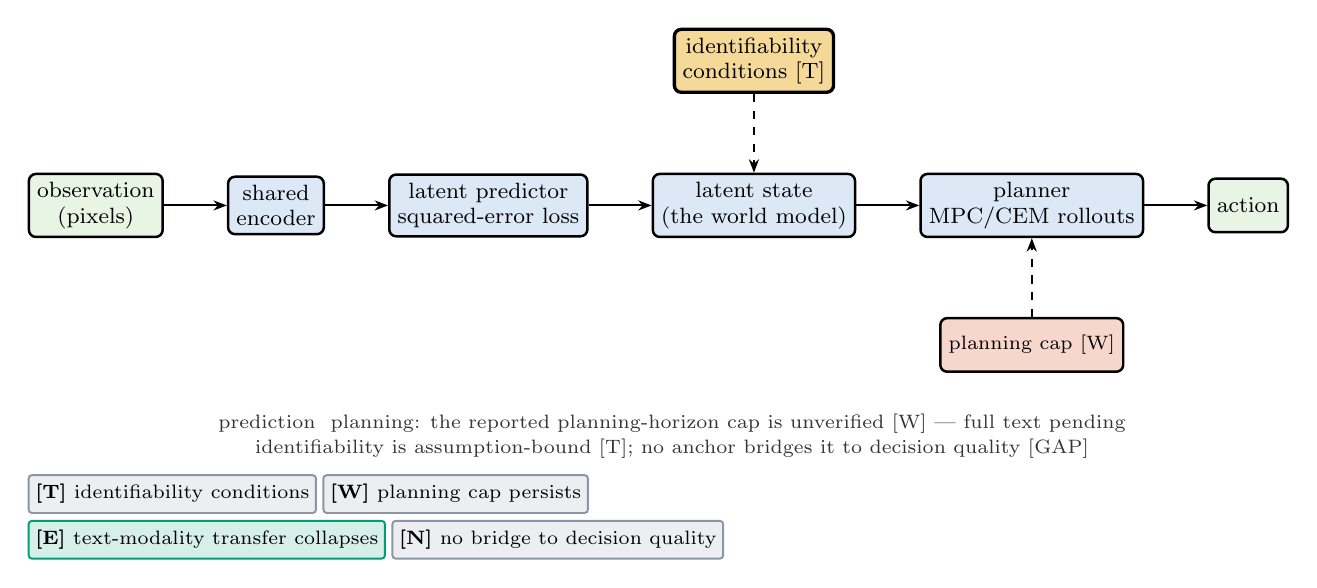
\begin{tikzpicture}
% ===== chain =====
\node[rs/gData] (obs) {observation\\(pixels)};
\node[rs/gModel, right=8mm of obs] (enc) {shared\\encoder};
\node[rs/gModel, right=8mm of enc] (pred) {latent predictor\\squared-error loss};
\node[rs/gModel, right=8mm of pred] (lat) {latent state\\(the world model)};
\node[rs/gModel, right=8mm of lat] (plan) {planner\\MPC/CEM rollouts};
\node[rs/gData, right=8mm of plan] (act) {action};
% ===== identifiability annotation (accent, above lat; dashed = claim to defend) =====
\node[rs/gAccent, above=10mm of lat] (ident) {identifiability\\conditions [T]};
% ===== planning-cap annotation (risk, below plan; numbers stay in the caption note) =====
\node[rs/gRisk, below=10mm of plan] (cap) {planning cap [W]};
% ===== edges =====
\draw[rs/gFlow] (obs.east) -- (enc.west);
\draw[rs/gFlow] (enc.east) -- (pred.west);
\draw[rs/gFlow] (pred.east) -- (lat.west);
\draw[rs/gFlow] (lat.east) -- (plan.west);
\draw[rs/gFlow] (plan.east) -- (act.west);
\draw[rs/gFlowD] (ident.south) -- (lat.north);
\draw[rs/gFlowD] (cap.north) -- (plan.south);
% ===== foot =====
\coordinate (mid) at ($(obs.center)!0.5!(act.center)$);
\node[rs/gFoot] at ([yshift=-8mm]mid |- cap.south) {prediction \figneq\ planning: the reported planning-horizon cap is unverified [W] --- full text pending\\identifiability is assumption-bound [T]; no anchor bridges it to decision quality [GAP]};
% --- evidence ribbon (P2): segments are claims already carried above; tag = the claim's class.
\rsRibbonBase{-3.4mm}
\rsRibbonRow{0mm}
\rsRibSeg{rsNoClaim}{\textbf{[T]} identifiability conditions}
\rsRibSeg{rsNoClaim}{\textbf{[W]} planning cap persists}
\rsRibbonRow{-5.8mm}
\rsRibSeg{rsVerified}{\textbf{[E]} text-modality transfer collapses}
\rsRibSeg{rsNoClaim}{\textbf{[N]} no bridge to decision quality}
\end{tikzpicture}
}
  \caption{Case 4: latent-predictive world-model planner. Accent = identifiability conditions $[T]$; the text layer renders prediction-is-not-planning as a caveat; the planning-horizon evidence is marked n/v in the section text pending a completed verification pass.}
  \label{fig:case-jepa}
\end{figure}

\subsection{Case 5: Discriminative classifier baseline}
\label{sec:case-classifier}
The deliberate non-generative control is a mapping head $P(y|x)$ whose L1 foregoes generation
entirely. Its reliability machinery carries calibration and
selective prediction inventories~\cite{id231108298,id250315850}, abstention
surveys~\cite{id240718418}, assumption-bound selective-prediction
guarantees~\cite{id260704430}, and a standing measure of the limit of instrumentation: runtime
monitors are a separate component, OOD detection alone does not close the
envelope~\cite{id221116158}, and monitoring itself can be evaded under ordinary task
pressure~\cite{id260930217}. \emph{Inherited failure:} no anchor in our evidence set benchmarks
a plain classifier baseline end-to-end against LLM and decision-model stacks on a shared task;
the quadrant limits drawn in \cref{fig:map} are therefore policy-relevant engineering judgment,
not measured comparisons. The same class-probability interface bridges back to the
decision-model case (\cref{sec:case-decision})~\cite{id261002267}.

\begin{figure}[h!]
  \centering
  \resizebox{\linewidth}{!}{% figures/f_case_classifier.tex — Case-study sketch (pack 5): discriminative classifier baseline.
% Grammar: figures/style_v2_tokens.tex (v8 token grammar).
% Roles: input / class probabilities / label / abstain = rs/gData; encoder + mapping head =
%   rs/gModel; selective gate = rs/gAccent (the ONE ledger-defended item, [T]); OOD + runtime
%   monitor = rs/gInfra (monitors are a distinct component, not a model).
% Chain: input x -> masked-pretrain encoder -> P(y | x) mapping head -> class probabilities ->
%   selective gate (risk-budget threshold) -> label / abstain; the monitor feeds the gate, and an
%   evasion lane (task pressure -> monitor, solid attack arrow) makes the monitor an untrusted
%   input to the gate. No second colour: the pressure block is a text label, not a role tile.
% Accent: the ONE yellow = threshold-from-risk-budget selective prediction [T] — assumption-bound.
% label: fig:case-classifier   (figure env + \label live in main.tex; case-studies slot, owner wires)
%
% CAPTION NOTE — items the paper must defend (state these in the caption):
%   1. [S] calibration / UQ / abstention inventories are LLM-centric (2503.15850 + 2311.08298,
%      abstention taxonomy 2407.18418); no anchor runs a plain classifier vs LLM/decision stacks
%      on a shared task [GAP] — comparability limit, not a performance claim;
%   2. [T] risk-budget threshold (2607.04430): provable alignment under assumptions only; bridges
%      to the conformal line (2405.01563) and the forms case;
%   3. [E] OOD detection alone insufficient — runtime monitors are a distinct component (2211.16158);
%      monitors themselves evadable under ordinary task pressure (2609.30217): the assurance layer
%      is part of the attack surface;
%   4. L4 contract = class probabilities, calibrated or not — same single-pass primitive as the
%      decision-model case (2610.02267's interface).
% Fonts >= 7.5pt; math glyphs measure ~0.92x nominal (CMSY/CMR quirk) so symbols use 8.2pt.
\providecommand{\figsep}{{\fontsize{8.2}{10}\selectfont $|$}}
\providecommand{\figplus}{{\fontsize{8.2}{10}\selectfont $+$}}
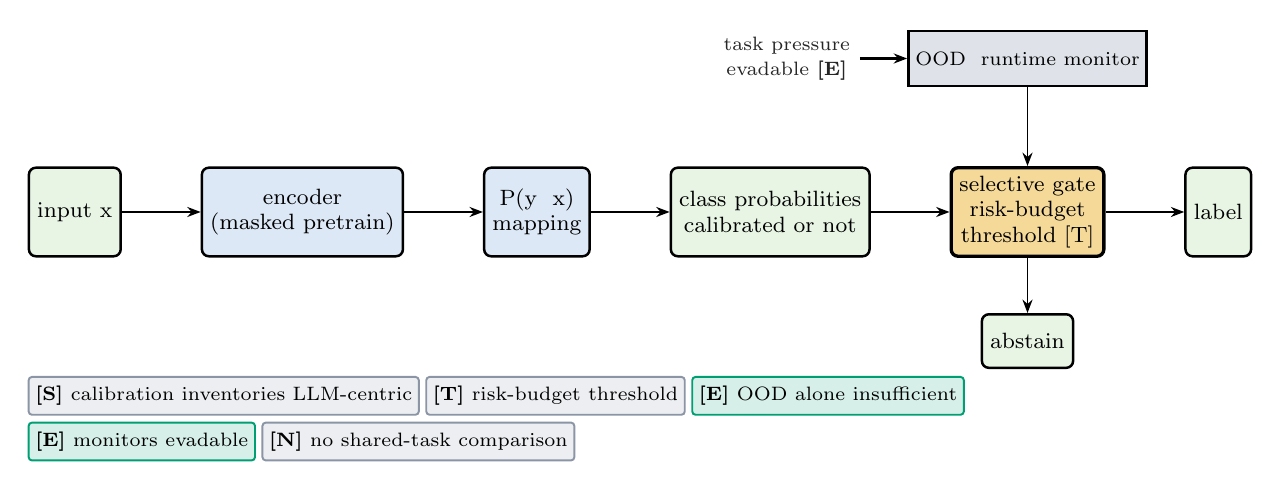
\begin{tikzpicture}
% uniform row height (the 3-line gate set the band; all six boxes match it)
\node[rs/gData, minimum height=32pt] (in1) {input x};
\node[rs/gModel, right=10mm of in1, minimum height=32pt] (enc) {encoder\\(masked pretrain)};
\node[rs/gModel, right=10mm of enc, minimum height=32pt] (map) {P(y \figsep\ x)\\mapping};
\node[rs/gData, right=10mm of map, minimum height=32pt] (prb) {class probabilities\\calibrated or not};
\node[rs/gAccent, right=10mm of prb, minimum height=32pt] (gate) {selective gate\\risk-budget\\threshold [T]};
\node[rs/gData, right=10mm of gate, minimum height=32pt] (lab) {label};
\node[rs/gData, below=7mm of gate] (abs) {abstain};
% ===== OOD + runtime monitor (feeds the gate) =====
\node[rs/gInfra, above=10mm of gate] (mon) {OOD \figplus\ runtime monitor};
% ===== evasion lane (E1): the monitor is an INPUT to the gate, so the gate inherits its
% evasion rate. Plain solid attack arrow into mon.west (no second colour: the role tokens keep
% their meaning; the pressure block is text, not a new tile). Numbers stay in the L5 prose/caption.
\node[anchor=east, align=center, font=\fontsize{7.5}{9.0}\selectfont, text=black!85]
  (tp) at ([xshift=-6mm]mon.west) {task pressure\\evadable \textbf{[E]}};
\draw[-{Stealth[length=1.7mm]}, line width=1.0pt, draw=black] (tp.east) -- (mon.west);
% ===== edges =====
\draw[rs/gFlow] (in1.east) -- (enc.west);
\draw[rs/gFlow] (enc.east) -- (map.west);
\draw[rs/gFlow] (map.east) -- (prb.west);
\draw[rs/gFlow] (prb.east) -- (gate.west);
\draw[rs/gFlow] (gate.east) -- (lab.west);
\draw[rs/gFlow] (gate.south) -- (abs.north);
\draw[rs/gFlow] (mon.south) -- (gate.north);
% L4 nuance now lives inside the prb node text ("calibrated or not") — no orphan edge label
% (foot removed: both lines restated ribbon chips already on the card; the evasion lane carries it)
% --- evidence ribbon (P2): segments are claims already carried above; tag = the claim's class.
\rsRibbonBase{-3.4mm}
\rsRibbonRow{0mm}
\rsRibSeg{rsNoClaim}{\textbf{[S]} calibration inventories LLM-centric}
\rsRibSeg{rsNoClaim}{\textbf{[T]} risk-budget threshold}
\rsRibSeg{rsVerified}{\textbf{[E]} OOD alone insufficient}
\rsRibbonRow{-5.8mm}
\rsRibSeg{rsVerified}{\textbf{[E]} monitors evadable}
\rsRibSeg{rsNoClaim}{\textbf{[N]} no shared-task comparison}
\end{tikzpicture}
}
  \caption{ Case 5: discriminative classifier baseline. Accent = risk-budget selective gate $[T]$; the gate consumes the OOD + runtime monitor, so the monitor's failure is the gate's: ordinary task pressure evades the monitor $[E]$ (\cite{id260930217}), making the assurance layer part of the attack surface rather than above it. OOD detection alone is insufficient $[E]$; cross-class comparability to LLM and decision-model stacks remains a named gap in the ledger.}
  \label{fig:case-classifier}
\end{figure}

\subsection{Case 6: Rules / formal-verification pipeline}
\label{sec:case-forms}
This is the null-instance discipline case: our evidence base contains no case-study-grade
anchor for a production rules-only or formally-verified AI pipeline, and \cref{sec:protocol}
records that as an honest null. What we hold instead are three verified enforcement classes:
deterministic schema/grammar enforcement at L4
\cite{id230513971,jsonschemabench2025,xgrammar2024}, verifier-failure evidence at
L5~\cite{id260601066} (validity $\neq$ truth applies to the verification layer itself), and
Redline-style risk-budgeted serving-configuration selection~\cite{id260933887} (a
configuration-selection class adjacent to Case 2's serving lanes, outside the formal
loop). \emph{Inherited failure:} statistical guarantee machinery (conformal abstention,
provable-alignment, Learn-Then-Test) is uniformly theory-class in our evidence; no independent
empirical evaluation of the formal loop over a learned model is in our evidence set.

\begin{figure}[h!]
  \centering
  \resizebox{\linewidth}{!}{% figures/f_case_forms.tex — Case-study sketch (pack 6): rules / constrained-decision pipeline.
% Grammar: figures/style_v2_tokens.tex (v8 token grammar).
% Roles: task / verdict+certificate = rs/gData; generative proposal = rs/gModel; formal validator =
%   rs/gAccent (the ONE ledger-defended item, [E]); statistical wrapper = neutral claim box
%   (rs/caseNote: gray dashed = claim-to-defend, mirrors f_fam_energy's [GAP] box; not a role);
%   fuzzer-found verifier gaps = the paired-verdict trace above the validator (ink only: filled
%   square = ACCEPT under the wider encoding, open square = REJECT under the narrower one; no
%   second colour, no rates).
% Chain: task under explicit spec -> generative proposal (grammar-constrained decoding) -> formal
%   validator (checks encoded constraints) -> verdict + certificate.
% Accent: yellow = deterministic validity enforcement [E] (schema-level / grammar-constrained).
% Dashed wires = claims-to-defend: statistical wrapper [T] qualifies learned components; the
%   fuzzer-found verifier-gap note [E] (validity != truth).
% label: fig:case-forms   (figure env + \label live in main.tex; case-studies slot, owner wires)
%
% CAPTION NOTE — items the paper must defend (state these in the caption):
%   1. HONEST NULL: no production rules-only / formally-verified pipeline anchor exists in our
%      build — this figure is our template instance, not a vendor reconstruction [GAP];
%   2. [E] syntax-level enforcement 2305.13971 / 2501.10868 / 2411.15100: validity guarantees are
%      relative to the encoded constraints, and enforced rules can be formally sound but factually
%      wrong;
%   3. [E] verifiers themselves fail (2606.01066): fuzzing finds verifier gaps — the validation
%      layer relocates rather than removes error;
%   4. [T] statistical wrappers (2609.33887 reference-relative risk; 2405.01563 conformal) are
%      assumption-bound and reference-relative — the reference itself may be wrong;
%   5. no anchor evaluates a formal verifier wrapping a learned model in a closed loop [GAP].
% Fonts >= 7.5pt; math glyphs measure ~0.92x nominal (CMSY/CMR quirk) so symbols use 8.2pt.
\providecommand{\figplus}{{\fontsize{8.2}{10}\selectfont $+$}}
\providecommand{\figneq}{{\fontsize{8.2}{10}\selectfont $\ne$}}
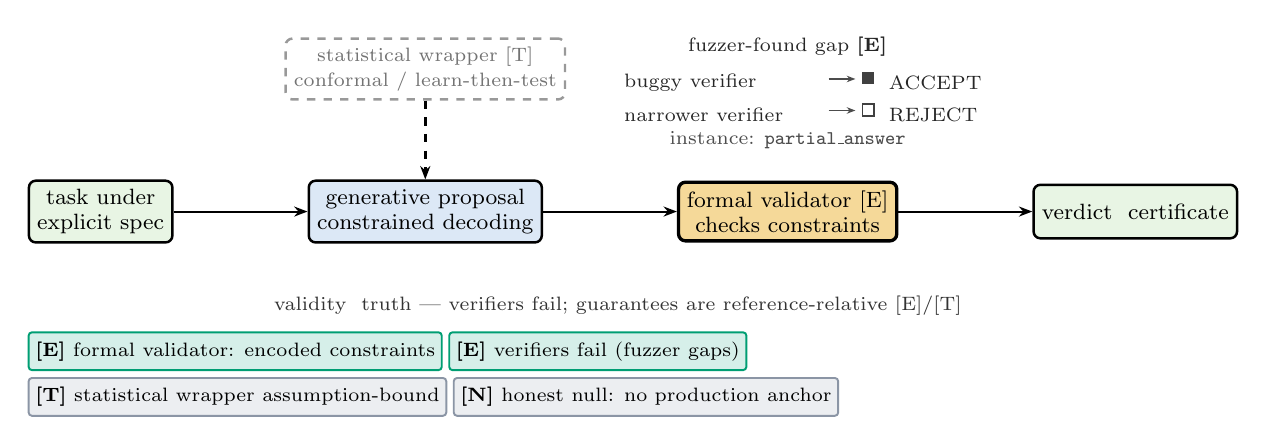
\begin{tikzpicture}
% claim-to-defend box (neutral, mirrors f_fam_energy's [GAP] pattern): not a role token, not the accent
\tikzset{rs/caseNote/.style={rounded corners=2.5pt, draw=black!40, line width=0.9pt, dashed,
  fill=white, align=center, inner sep=3pt, font=\fontsize{7.5}{9.0}\selectfont, text=black!55}}
% ===== chain =====
\node[rs/gData] (in1) {task under\\explicit spec};
\node[rs/gModel, right=17mm of in1] (gen) {generative proposal\\constrained decoding};
\node[rs/gAccent, right=17mm of gen] (val) {formal validator [E]\\checks constraints};
\node[rs/gData, right=17mm of val] (ver) {verdict \figplus\ certificate};
% ===== statistical wrapper (above proposal, dashed claim) =====
\node[rs/caseNote, above=10mm of gen] (wrap) {statistical wrapper [T]\\conformal / learn-then-test};
% ===== paired-verdict trace (F1): the same completion, two encodings of the constraint =====
% The divergence IS the claim: a wider encoded language ACCEPTs what a narrower one REJECTs, so
% "valid" is relative to the encoded constraints and the guard relocates error rather than
% removing it. Verdict markers are filled (accepted) vs open (rejected) -- presence/absence, no
% second colour. The instance label is the anchor's own example; no counts, no rates.
\coordinate (trc) at ($(val.north)+(-22mm,4mm)$);
\begin{scope}[shift={(trc)}, x=1mm, y=1mm]
\node[anchor=base, font=\fontsize{7.5}{9.0}\selectfont, text=black!85] at (22,12.4)
  {fuzzer-found gap \textbf{[E]}};
\node[anchor=west, font=\fontsize{7.5}{9.0}\selectfont, text=black!85] at (0,8.4) {buggy verifier};
\draw[-{Stealth[length=1.1mm]}, line width=0.6pt, draw=black!70] (27.2,8.9) -- (30.6,8.9);
\fill[black!75] (31.5,8.25) rectangle ++(1.5,1.5);
\node[anchor=west, font=\fontsize{7.5}{9.0}\selectfont, text=black!85] at (33.6,8.4) {ACCEPT};
\node[anchor=west, font=\fontsize{7.5}{9.0}\selectfont, text=black!85] at (0,4.4) {narrower verifier};
\draw[-{Stealth[length=1.1mm]}, line width=0.6pt, draw=black!70] (27.2,4.9) -- (30.6,4.9);
\draw[black!75, line width=0.7pt, fill=white] (31.5,4.25) rectangle ++(1.5,1.5);
\node[anchor=west, font=\fontsize{7.5}{9.0}\selectfont, text=black!85] at (33.6,4.4) {REJECT};
\node[anchor=base, font=\fontsize{7.5}{9.0}\selectfont, text=black!70] at (22,0.6)
  {instance: \texttt{partial\_answer}};
\end{scope}
% ===== edges =====
\draw[rs/gFlow] (in1.east) -- (gen.west);
\draw[rs/gFlow] (gen.east) -- (val.west);
\draw[rs/gFlow] (val.east) -- (ver.west);
\draw[rs/gFlowD] (wrap.south) -- (gen.north);
% ===== foot (clears the validator); the honest-null line lived in the [N] chip already =====
\coordinate (mid) at ($(in1.center)!0.5!(ver.center)$);
\node[rs/gFoot] at ([yshift=-8mm]mid |- val.south) {validity \figneq\ truth --- verifiers fail; guarantees are reference-relative [E]/[T]};
% --- evidence ribbon (P2): segments are claims already carried above; tag = the claim's class.
\rsRibbonBase{-3.4mm}
\rsRibbonRow{0mm}
\rsRibSeg{rsVerified}{\textbf{[E]} formal validator: encoded constraints}
\rsRibSeg{rsVerified}{\textbf{[E]} verifiers fail (fuzzer gaps)}
\rsRibbonRow{-5.8mm}
\rsRibSeg{rsNoClaim}{\textbf{[T]} statistical wrapper assumption-bound}
\rsRibSeg{rsNoClaim}{\textbf{[N]} honest null: no production anchor}
\end{tikzpicture}
}
  \caption{ Case 6: rules / formal-verification pipeline. Accent = formal validator $[E]$ (validity relative to encoded constraints). Above it, a paired-verdict trace: the same completion (\texttt{partial\_answer}) is ACCEPTed under a buggy encoding and REJECTed under a narrower one, so the guard relocates error rather than removing it (\cite{id260601066}) --- the narrower verdict is not ``correct'', only narrower; filled/open markers carry the verdicts, no second colour. This card is a template instance: an honest null, since no production formal-verification anchor exists in our evidence base.}
  \label{fig:case-forms}
\end{figure}

\subsection{Case 7: Production diffusion-LLM serving}
\label{sec:case-diffusion}
Diffusion LLMs have production instances, and the reliability research has not caught up.
Mercury~2.5 has been served since 2026-09-08~\cite{inception2026mercury25}, and the open-weight
branch is as concrete: LLaDA2.x ships under Apache-2.0 at 16B and 100B-MoE with its own inference
engine and block-parallel decode~\cite{llada2026two}. Declared and deployed rates diverge: 1,107
tok/s declared for 2.5 \cite{inception2026mercury25} \evvendor{} against 770 tok/s on a
fixed-workload independent instrument and 141 tok/s at router
P50~\cite{artificialanalysis2026mercury25,openrouter2026mercury} \evindep{}. Two independent
instruments differ fivefold on one model, so the vendor figure reads as a ceiling on an undisclosed
workload.

The levers split along that hosted/open-weight line. The operating-point procedure of \cref{sec:l5-bridge} is
executable only where the engine is yours: on LLaDA2 you choose sampler and step count, on the
hosted endpoint neither is a request parameter. The current hosted generation
(Mercury~3\footnote{Mercury~3 was announced 2026-10-19, two days after our 2026-10-17 cutoff. It
enters this card as a \textsf{[V]} vendor claim only and is not corpus evidence.}) returns text,
usage, and a stream of \emph{revisions} rather than appended tokens, and its request schema
carries no seed, no \texttt{logprobs} or \texttt{top\_logprobs}, no $n$ and no step count, with
temperature floored at 0.5~\cite{inception2026mercury3}. With no per-token score to threshold, the
only acceptance surface left is agreement over $k$ whole outputs. The same vendor's typed endpoint is the
counter-example: \texttt{choice}/\texttt{score}/\texttt{noul} with probabilities, and
\evindep{ranked 3/135 on an independent decision board}~\cite{jevbench2026board}. Reliability here
is bought at L4, by choosing the endpoint.

\emph{What this instance leaves unmeasured:} Mercury~3 postdates our cutoff, so no independent
quality evaluation of it exists, and for 2.5 the only independent quality signal is a single index
score (12, against 21/22/17 on the peers it names), so the hosted generation's quality evidence is
thin and mostly vendor-reported. The case concerns the contract and the evidence record. No sampler-variance
or NFE study is published either; the inherited failure is sampler sensitivity \emph{made
unobservable}, not merely present. Nor does the instance show that parallel refinement buys
reliability: latency shape is not an assurance property, and the open-weight branch is the only
place where the sampler can be held fixed.

\begin{figure}[h!]
  \centering
  \resizebox{\linewidth}{!}{% figures/f_case_diffusion.tex — Case-study sketch (pack 7): production diffusion-LLM serving.
% Grammar: figures/style_v2_tokens.tex (v8 token grammar).
% Roles: prompt / text = rs/gData (payload); the denoising lanes are INK, not a role — a pass is a
%   schedule, not a component, and no role token should be spent on one; the four
%   contract cells = rs/gInfra (sharp rectangle = a service surface, not a store, not a model);
%   edges = rs/gFlow (thin gray arrows); labels = rs/gTiny.
% Left: L positions refined in parallel over T vendor-set passes — pass 1 mostly unresolved (?),
%   pass T fully settled; filled cell = a settled position. Step counts are symbolic; no wall-clock
%   is drawn, and no clock/axis tick appears anywhere in the card.
% Right: what the hosted text endpoint withholds — temperature floored at 0.5, no seed, no
%   logprobs, a stream of revisions rather than appended tokens. The dashed vermillion leader
%   marks the CONTESTED inference [C]: with no token score, the only acceptance surface left is
%   whole-output agreement over k resamples. The schema silence is [V]; the consequence is ours.
% label: fig:case-diffusion   (figure env + \label live in cases.tex, Case 7)
%
% CAPTION NOTE — items the paper must defend:
%   1. [V] contract surface (vendor OpenAPI, read 2026-10-20): temperature in [0.5, 1.0] with
%      out-of-range values reset to the default; no seed / logprobs / top_logprobs / n; no step
%      count or schedule parameter; the diffusing stream is a view of intermediate refinement,
%      not appended tokens;
%   2. [V] throughput declared 1,107 tok/s (Mercury 2.5, 2026-09-08) vs [E] 770 tok/s on a
%      fixed-workload independent instrument and 141 tok/s at router P50 — do not average them;
%   3. [C] acceptance-collapse: schema silence about scores is [V], the consequence for the L5
%      gate is our inference;
%   4. [N] no independent quality evaluation of the hosted generation exists at cutoff.
% Fonts >= 7.5pt; math glyphs measure ~0.92x nominal (CMSY/CMR quirk) so symbols use 8.2pt.
\providecommand{\figge}{{\fontsize{8.2}{10}\selectfont $\ge$}}
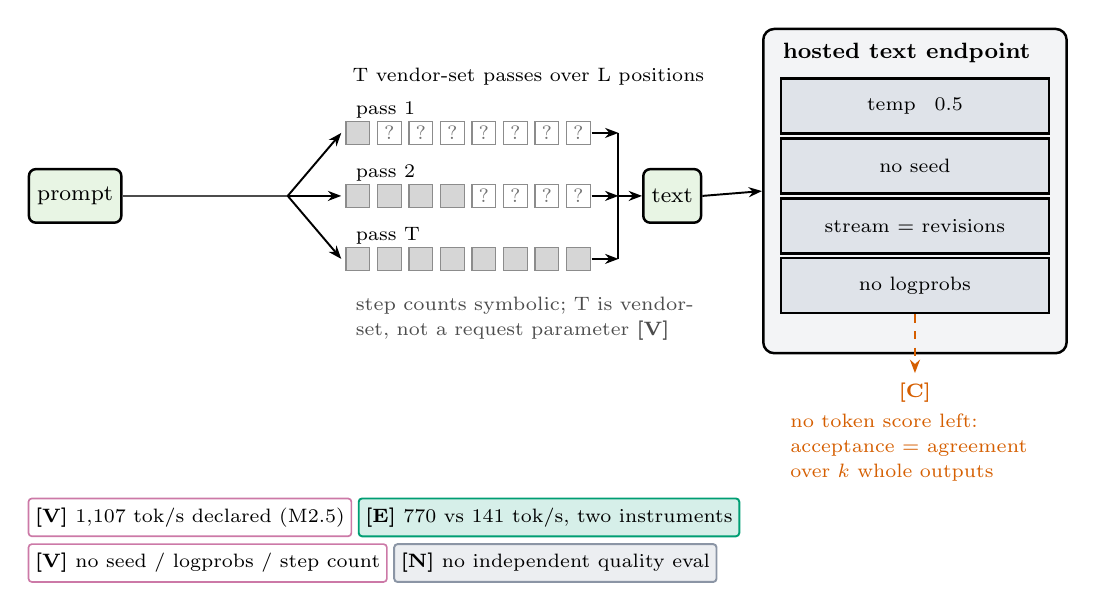
\begin{tikzpicture}[x=1mm,y=1mm]
\pgfdeclarelayer{rsbg}\pgfsetlayers{rsbg,main}  % panel tint renders UNDER its cells
% ===== left: prompt -> parallel denoising lanes -> text =====
\node[rs/gData] (in1) {prompt};
\node[rs/gTiny, anchor=west] at (34,15.2) {T vendor-set passes over L positions};
\foreach \y/\lab/\settled in {8/1/1, 0/2/4, -8/T/8} {
  \node[rs/gTiny, anchor=west] at (34.4,{\y+2.9}) {pass \lab};
  \foreach \i in {0,...,7} {
    \pgfmathsetmacro{\cx}{35.9+4*\i}
    \ifnum\i<\settled
      \draw[draw=black!45, line width=0.4pt, fill=black!16]
        (\cx,\y) ++(-1.5,-1.5) rectangle ++(3,3);
    \else
      \draw[draw=black!45, line width=0.4pt, fill=white]
        (\cx,\y) ++(-1.5,-1.5) rectangle ++(3,3);
      \node[inner sep=0pt, font=\fontsize{7.5}{9.0}\selectfont, text=black!55] at (\cx,\y) {?};
    \fi
  }
}
% edges: one fan out of the prompt into the three lanes, one comb back into the text box
\draw[black!70, line width=0.7pt] (in1.east) -- (27,0);   % trunk: no arrowhead at a bare fork
\foreach \y in {8,0,-8} {
  \draw[rs/gFlow] (27,0) -- (33.8,\y);
  \draw[rs/gFlow] (65.6,\y) -- (69,\y);
}
\draw[black, line width=0.7pt] (69,8) -- (69,-8);
\draw[rs/gFlow] (69,0) -- (72,0);
\node[rs/gData, anchor=west] (out) at (72,0) {text};
% honesty line under the lanes (the caption repeats it; the card must not imply a measured clock)
\node[anchor=north west, align=left, text=black!70, text width=44mm,
      font=\fontsize{7.5}{9.0}\selectfont] at (34.4,-11.6)
  {step counts symbolic; T is vendor-set, not a request parameter \textbf{[V]}};
% ===== right: the hosted endpoint's contract surface (container of four cells) =====
\node[rs/gInfra, anchor=west, minimum width=34mm] (c1) at (89.5,11.4) {temp \figge\, 0.5};
\node[rs/gInfra, anchor=west, minimum width=34mm] (c2) at (89.5,3.8)  {no seed};
\node[rs/gInfra, anchor=west, minimum width=34mm] (c3) at (89.5,-3.8) {stream $=$ revisions};
\node[rs/gInfra, anchor=west, minimum width=34mm] (c4) at (89.5,-11.4) {no logprobs};
\coordinate (padtop) at ([yshift=3.5pt]c1.north);
\begin{pgfonlayer}{rsbg}
  \node[rs/gPanelFill, fit=(c1)(c4)(padtop)] {};
\end{pgfonlayer}
\node[rs/gPanelEdge, fit=(c1)(c4)(padtop),
      label={[rs/gPanelTitle, xshift=4pt, yshift=-9pt]north west:hosted text endpoint}] (panel) {};
\draw[rs/gFlow] (out.east) -- (panel.west);
% [C]: the score is absent, so the acceptance surface collapses — our inference, not the schema.
% The leader leaves the bottom cell vertically, clears the panel border once, and lands outside it.
\draw[rsContested, dashed, line width=0.9pt, -{Stealth[length=1.7mm]}]
  (c4.south) -- (c4.south |- 0,-22.5);
\node[rs/gTiny, anchor=north, text=rsContested] at (c4.south |- 0,-22.5) {\textbf{[C]}};
\node[anchor=north west, align=left, text=rsContested, text width=34mm,
      font=\fontsize{7.5}{9.0}\selectfont] at (89.6,-26.5)
  {no token score left: \mbox{acceptance} $=$ agreement over $k$ whole outputs};
% --- evidence ribbon (P2): segments are claims already carried above; tag = the claim's class.
\rsRibbonBase{-3.4mm}
\rsRibbonRow{0mm}
\rsRibSeg{rsVendor}{\textbf{[V]} 1,107 tok/s declared (M2.5)}
\rsRibSeg{rsVerified}{\textbf{[E]} 770 vs 141 tok/s, two instruments}
\rsRibbonRow{-5.8mm}
\rsRibSeg{rsVendor}{\textbf{[V]} no seed / logprobs / step count}
\rsRibSeg{rsNoClaim}{\textbf{[N]} no independent quality eval}
\end{tikzpicture}
}
  \caption{ Case 7: production diffusion-LLM serving. Left: $L$ positions refined in parallel over $T$ vendor-set passes --- filled = settled, ? = still unresolved, step counts symbolic and no wall-clock drawn. Right: the hosted text endpoint's acceptance surface: temperature floored at 0.5, no seed, no logprobs, a stream of revisions rather than appended tokens. The vermillion dashed leader marks the contested inference $[C]$: with no token score, acceptance reduces to agreement over $k$ whole outputs --- the schema silence is $[V]$, the consequence for the L5 gate is ours. Throughput is vendor/independent paired ($1{,}107$ tok/s declared vs 770 tok/s on a fixed-workload instrument and 141 tok/s at router P50); Mercury~3 postdates the cutoff, so no independent evaluation of it exists; 2.5 carries one independent index score.}
  \label{fig:case-diffusion}
\end{figure}

\subsection{Cross-case synthesis}
\label{sec:crosscase}
Three regularities emerge, and each survives a row-by-row read of \cref{tab:crosscase}. First,
the case cards' \emph{strongest} reliability moves sit above the objective, at L4--L5 for five
of seven instances (1, 2, 5, 6, 7) and L2 for the two representational ones (3, 4), rather than at
the objective's home layer. That pattern is an argument for cross-layer engineering, and against
committing to a single objective family. Second, the
last engineering move in each case sits above the mechanism it secures: the decision case needs
the L5 gate, and the formal case needs its L5 wrapper re-evaluated. Row~7 is the new information
in this table: its reliability move is procurement at L4 --- choose the endpoint that reports
scores. Third, two of the three families \cref{fig:evidence} surfaces as
most-contested appear here --- calibration direction and latent-prediction stability --- so the
ledger makes the paper's uncertainty legible rather than uniform.

\begin{table}[!t]
\centering\small
\begin{tabular}{@{}p{4.0cm}p{5.6cm}p{5.6cm}@{}}
\toprule
Case & Strongest reliability move & Worst failure the home layer cannot close \\
\midrule
1 RAG-LLM assistant & grounding gate + abstention machinery ([E]~\cite{id260935794}; [T]~\cite{id240501563}) & hallucination intrinsic to the AR objective; mitigation composition unmeasured \\
2 Decision-model serving & typed closed contract + proper-scoring rules ([V] Laya; [E]~\cite{rauk2026jevbenchmark,id261019811}) & interface instability: \evindep{30\% of answers flip under option reversal~\cite{id261002267}}; calibration direction contested~\cite{id260933843}; \evindep{gate misses its 10\% accepted-error target} \\
3 Hybrid specialist & structured, checkable fields returned by the specialist components ([V]~\cite{interfaze2026}) & cross-component error propagation unmeasured (named gap); all evaluation evidence vendor-reported \\
4 JEPA planner & identifiability-under-assumptions guarantees ([T]~\cite{klindt2026lejepa,identifiability2026}) & an unverified report of a planning-horizon cap; all quantities n/v ([W]~\cite{id260939235}); an independent evaluation reports latent-prediction instability on ambiguous text ([E]~\textsf{[C]}~\cite{id260723531}) \\
5 Classifier baseline & calibration/abstention/monitoring inventory ([S, T]) & monitor evasion under task pressure ([E]~\cite{id260930217}); instrumentation needs its own threat model \\
6 Rules / formal & deterministic validity enforcement ([E]) + distribution-free wrappers ([T]) & validity $\neq$ truth: verifiers themselves fail ([E]~\cite{id260601066}); honest null on formal loops \\
7 Diffusion-LLM serving & endpoint choice as the reliability move: the typed endpoint reports scores ([V] docs; [E] rank 3/135~\cite{jevbench2026board}) where the text endpoint reports none & sampler schedule is vendor-side --- no step count, seed or token score, so sampler variance cannot be held fixed (named gap) \\
\bottomrule
\end{tabular}
\caption{Cross-case comparison. Evidence classes: \cref{sec:protocol}. The third column names the mechanism that the instance's own layer cannot close.}
\label{tab:crosscase}
\end{table}

\FloatBarrier

\section{Task Selection Framework}\label{sec:selection}
\begin{figure}[t]
  \centering
  % \includegraphics[width=\linewidth]{figures/f2_task_map.pdf}
  % figures/f2_task_map_draft.tex — F2 v4 (2026-10-19): V4 redesign C1 "two probes".
% Task-selection map, 2x2 over answer-space openness (x) and cost of error (y).
% Structural grammar: one solid frame, solid hairline dividers, ONE black!6 band + 0.9pt top rule
% for the escalation row (no amber anywhere: the band a region cannot carry a ledger row).
% The map is shown USED: two probes from our own case set are placed on the axes
%   case 1 RAG assistant   = high cost x open-ended
%   case 2 decision serving = high cost x well-defined
% (case 2 is placed high-cost, not low-cost as the ideas memo had it: a typed decision acts with
% no human reader in the loop -- cases.tex -- so a low-cost placement would contradict the case.)
% One dashed elbow from probe 1 to the reversibility modifier callout = the reversibility modifier,
% not a measured trajectory (it shows which lever would move the placement, so it ends on that lever).
% The four modifiers sit in one right-hand column behind a single bracket to the frame (they modify
% placement anywhere; per-tile arrows implied a false specificity).
% Four corner labels and the two-line foot are deleted (axes labels + caption carry them).
% label: fig:map   (figure env + \label live in main.tex)
% CAPTION (main.tex) needs: "[S] quadrant modes are candidates, not guarantees"; "probe placements
% are ours (illustrative), the dashed elbow is a claim-to-defend, not a measured boundary";
% "modifier callouts are claims-to-defend"; "escalation band = high-error-cost row: defer, verify,
% escalate"; "both axes qualitative".
% Fonts >= 7.5pt; natural width ~153mm.
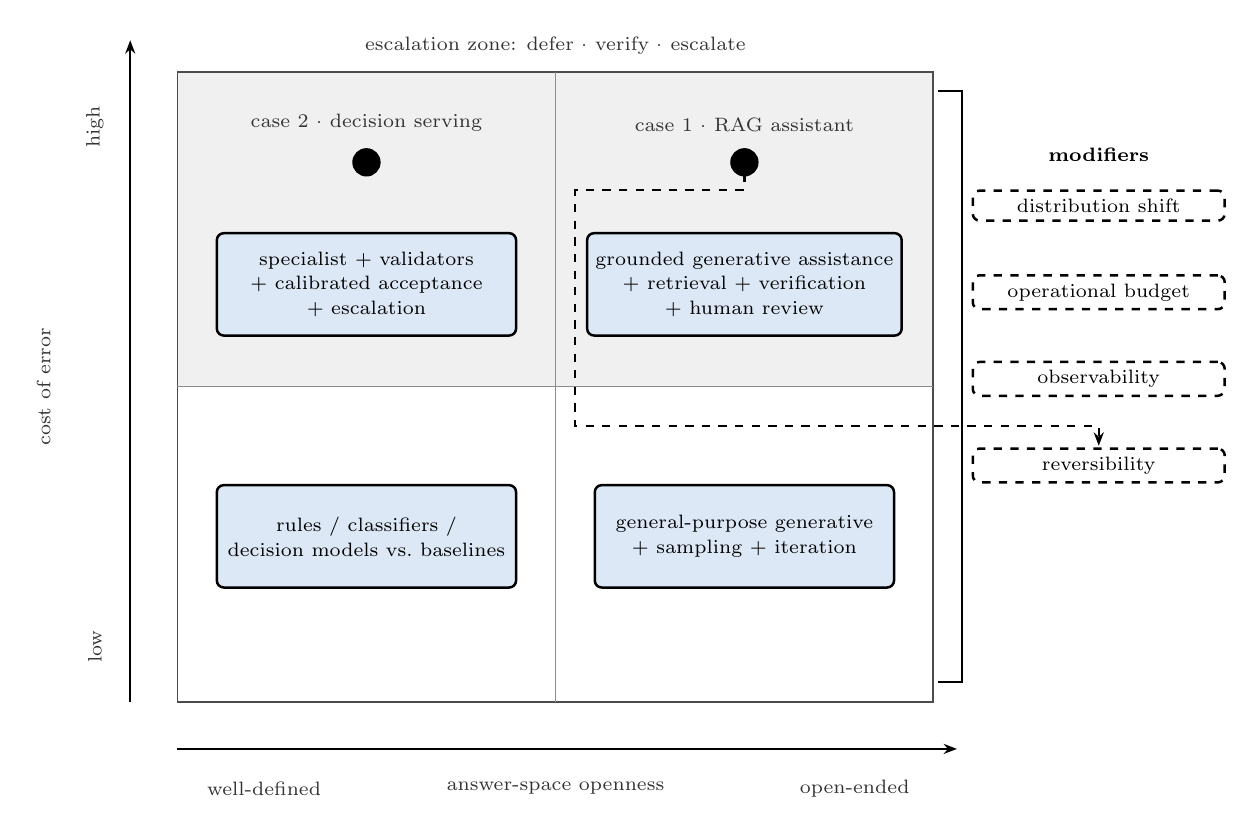
\begin{tikzpicture}[x=1mm,y=1mm]
\tikzset{
  rs/f2callout/.style={rounded corners=2.5pt, draw=black, dashed, line width=0.9pt, fill=white,
    align=center, inner sep=3pt, font=\fontsize{7.5}{9.0}\selectfont},
  rs/f2lbl/.style={font=\fontsize{7.5}{9.0}\selectfont, text=black!80},
  rs/f2tile/.style={rs/gModel, minimum width=38mm, minimum height=13mm,
    font=\fontsize{7.5}{9.0}\selectfont},
  rs/f2probe/.style={circle, fill=black, inner sep=0pt, minimum size=3.6mm},
}
% ===== escalation zone: high-error-cost row, neutral fill + heavier top rule (the ONE emphasis) =====
\fill[black!6] (0,40) rectangle (96,80);
\draw[line width=0.9pt, draw=black] (0,80) -- (96,80);
% ===== frame + quadrant dividers (structure = solid hairlines) =====
\draw[line width=0.7pt, draw=black!70] (0,0) rectangle (96,80);
\draw[line width=0.4pt, draw=black!45] (48,0) -- (48,80);
\draw[line width=0.4pt, draw=black!45] (0,40) -- (96,40);
% ===== axes =====
\draw[rs/gFlow] (0,-6) -- (99,-6);
\draw[rs/gFlow] (-6,0) -- (-6,84);
\node[rs/f2lbl] at (11,-11) {well-defined};
\node[rs/f2lbl] at (48,-11) {answer-space openness};
\node[rs/f2lbl] at (86,-11) {open-ended};
\node[rs/f2lbl, rotate=90] at (-10.5,7)  {low};
\node[rs/f2lbl, rotate=90] at (-10.5,73) {high};
\node[rs/f2lbl, rotate=90] at (-17,40)   {cost of error};
% ===== escalation-zone label (band, high-error row) — above the frame by necessity: the label is
% 55mm wide and the quadrant divider at x=48 runs the full height, so any in-frame position puts a
% rule through the text (measured: 1 line/text crossing). It labels the band from outside =====
\node[rs/f2lbl, anchor=south] at (48,81) {escalation zone: defer \textperiodcentered\ verify \textperiodcentered\ escalate};
% ===== candidate-mode tiles (candidate operating modes, not guarantees) =====
\node[rs/f2tile] at (24,53) {specialist + validators\\+ calibrated acceptance\\+ escalation};
\node[rs/f2tile] at (72,53) {grounded generative assistance\\+ retrieval + verification\\+ human review};
\node[rs/f2tile] at (24,21) {rules / classifiers /\\decision models vs.\ baselines};
\node[rs/f2tile] at (72,21) {general-purpose generative\\+ sampling + iteration};
% ===== two probes: our own cases placed on the axes =====
\node[rs/f2probe] (p1) at (72,68.5) {};
\node[rs/f2lbl, anchor=south] at (72,71.2) {case 1 \textperiodcentered{} RAG assistant};
\node[rs/f2probe] (p2) at (24,68.5) {};
\node[rs/f2lbl, anchor=south] at (24,71.2) {case 2 \textperiodcentered{} decision serving};
% one dashed elbow = the reversibility modifier (a shift, not a measured trajectory). It leaves the
% probe, drops through the open corridor at x=50.5 (clears the centre divider at 48 and the narrowed
% right-column tile at 53 by 2.5mm each), runs along y=35 (the empty band between the low-cost tiles
% at 26.5 and the quadrant divider at 40) and TERMINATES on the reversibility callout's north edge.
% It used to stop at (50.5,36) with its own "reversibility" label there, i.e. it dangled inside the
% low-cost row and named itself twice; the label now exists once, on the callout it points at.
\draw[rs/gFlowD] (72,67) -- (72,65) -- (50.5,65) -- (50.5,35) -- (117,35) -- (117,32.5);
% ===== modifier column: one bracket to the frame, no per-tile arrows =====
\draw[line width=0.7pt, draw=black] (96.6,2.5) -- (99.6,2.5) -- (99.6,77.5) -- (96.6,77.5);
\node[rs/f2lbl, anchor=south, font=\fontsize{7.5}{9.0}\selectfont\bfseries, text=black] at (117,67.4)
  {modifiers};
\node[rs/f2callout, minimum width=32mm] at (117,63) {distribution shift};
\node[rs/f2callout, minimum width=32mm] at (117,52) {operational budget};
\node[rs/f2callout, minimum width=32mm] at (117,41) {observability};
\node[rs/f2callout, minimum width=32mm] at (117,30) {reversibility};
\end{tikzpicture}

  \caption{ Task-selection map: quadrant mode lists are candidate operating modes [S]; the two probes are our own cases placed illustratively --- case 2 sits at high cost because a typed decision acts without a human reader in the loop --- and the dashed elbow runs from probe 1 to the reversibility callout --- it names the lever that would move the placement, not a measured trajectory; modifier callouts are claims-to-defend; the escalation band is the high-error-cost row (default response: defer, verify, escalate).}
  \label{fig:map}
\end{figure}
% Section 10: selection framework (P4)
The stack of \cref{sec:stack} tells you \emph{what a system is}, and this section tells a
practitioner \emph{what to build}. The selection framework routes by task; model preference is not
an axis. It is written as a
procedure because the assembly is the product. Each of the six steps hands the next a term it
cannot invent for itself, and the last one ends at a configuration whose residual risk is named
and owed.

\subsection{The two axes}
\label{sec:sel-axes}
The horizontal axis is \textbf{answer-space openness}: how far the correct answer set is from
enumerable at design time. Well-defined answer spaces support closed contracts (typed
decisions, validation); open-ended ones cannot be closed by any contract layer and must rely
on grounding and review (\cref{sec:case-rag}). We use \emph{openness of the
answer space}. Stochastic inference is a deployment knob; an axis built on it would re-ask the
determinism question and leave every reliability limit unaddressed.

The vertical axis is \textbf{cost of error}: the severity of a wrong output. Reversible low-stakes
outputs allow sampling or iteration strategies; irreversible high-stakes ones push the operating
point toward validated acceptance and human escalation, whichever objective family serves the
task. \cref{fig:map} draws the resulting quadrants and the escalation band.

\subsection{The procedure}
\label{sec:sel-procedure}
The procedure starts from the paper's one falsifiable cross-layer regularity: failures originate
where they are least catchable and are usually caught in the later columns of
\cref{fig:failmatrix}. Where the checks sit is therefore a decision the procedure makes. It
consumes the ledger.

\begin{enumerate}[leftmargin=1.6em, itemsep=2pt]
\item \textbf{Risk specification.} Fix the three terms that make ``reliable'' a claim in this
  paper: the envelope of failure kinds the system must not produce, the budget it must hold, and
  the assurance path that intervenes as it drifts (\cref{sec:reliability}). Mapped onto the
  framework, those terms are two axes---answer-space openness and error severity---plus two
  constraints, reversibility and operational budget: three claims, which the framework reads as
  four terms every later step reads.

\item \textbf{Placement.} Locate the task on \cref{fig:map}: how open the answer set is at design
  time, and what a wrong output costs. The coordinate is an analytic cut [J], the status the map
  gives its quadrant lists. Record the reason the placement holds rather than treating the
  quadrant as measured, and keep task openness separate from decoding stochasticity, which is a
  deployment knob (\cref{sec:reliability}).

\item \textbf{Modifier routes.} Walk the four placement modifiers --- distribution shift,
  reversibility, observability, operational budget --- plus the schedule route, which asks the
  question the axes never raise: \emph{which factorization does this contract have to inspect?}
  The schedule is not inherited from the objective; \cref{fig:schedule-atlas} draws the three
  factorizations as lanes, and \cref{sec:sel-modifiers}(v) states the route. Each route is stated
  with its evidence there; any of them can move the operating point without
  moving the axes, so the placement from Step~2 is provisional until they have been walked.

\item \textbf{Probe against the failure matrix.} For each failure kind in the envelope, find the
  row where it originates in \cref{fig:failmatrix} and ask which later column would catch it;
  where no column does, the candidate needs another layer or a narrower claim, and the residue is
  bracketed as the residual of \cref{fig:layer5-assur}. A candidate that verifies only at the
  layer where it operates is checking the wrong place by default: origins cluster at L2 while
  filled cells cluster in the last three columns. The two probes already on
  \cref{fig:map} are our own cases, and they are illustrative: they show what a filled placement
  looks like before any threshold exists.

\item \textbf{Archetype routes.} Read the quadrant's candidate modes and select one to carry:
  (low cost, well-defined) rules, classifiers and decision models benchmarked against baselines;
  (high cost, well-defined) specialist plus validators, calibrated acceptance and escalation;
  (high cost, open-ended) grounded generative assistance with retrieval, verification and human
  review; (low cost, open-ended) general-purpose generation with sampling and iteration. Two gated
  variants enter only where their precondition holds: latent-prediction planning under
  identifiability conditions (\cref{sec:case-jepa}), and rules or formal verification where an
  executable validator exists (\cref{sec:case-forms}). Then read the card of
  \cref{sec:familycards} --- what the objective optimizes, which task types it suits, which
  failure modes remain, which complementary layers cover the residual --- and the mechanism
  sketch for where the design's benefit comes from. The route fixes the objective family and the
  contract tier; it does not fix the schedule of Step~3.

\item \textbf{Budget covenant.} Convert the L0 budget into thresholds and escalation conditions
  with the existing [T]-class machinery --- conformal abstention \cite{id240501563},
  risk-controlled selective answering \cite{id260704430}, and risk-budgeted serving
  \cite{id260933887} --- then fit them on the operator's calibration set, reference configuration
  and correctness measure. The cutoff is the cost-based reject option, chosen to hold the error
  budget on the calibration distribution \cite{geifman2017selective}; never install it as a fixed
  universal constant (see also the contested-direction caveat \cite{id260933843}); the output is an
  \emph{operator}, not a ``safe zone''. Instrument it: monitors, abstention and escalation ladder,
  plus a scheduled evaluation plan that tracks shift and takeover attempts, the contested claims of
  \cref{tab:crosscase} included.
\end{enumerate}
What the six steps produce is a candidate operating mode with a checked residual-risk story.
The framework draws two lines: it treats ranking model classes against each other as a
category error (\cref{sec:stack}), and it holds escalation to the residual the evidence supports.

\subsection{Modifier routes}
\label{sec:sel-modifiers}
Four modifiers move the placement and leave the axes fixed. A fifth route, the schedule, does a
different job: it selects which factorization the contract inspects. All five are claims we have
to defend, and each answers a question the placement alone cannot settle.

\begin{description}[leftmargin=1.5em, itemsep=1pt]
\item[(i) Distribution shift.] Widens margins on the reliability side: a well-instrumented
  classifier degrades unpredictably under shift, making calibrated abstention the floor rather
  than a bonus \cite{id250315850,id221116158}. Shift is also the matrix's one ambiguous origin row,
  filed at L0 and stated as such (\cref{fig:failmatrix}).
\item[(ii) Reversibility.] Converts some high-error-cost placements back into the iterative
  regime, because repairable damage can wait for repair. The
  dashed elbow of \cref{fig:map} is this move drawn.
\item[(iii) Observability.] Determines whether the assurance layer gets signal at all; monitoring
  under low observability is one of the honest failed rows of \cref{sec:case-classifier}, where
  the monitor is evaded under ordinary task pressure \cite{id260930217}.
\item[(iv) Operational budget.] Constrains the acceptable cost of the safeguard chain itself; it
  constrains which configuration is even selectable, not how reliable it should be. A
  configuration that reaches target quality faster converts its margin into reliability budget
  (more candidates, more checks) rather than raw throughput; the schedule classes of
  \cref{fig:schedule-atlas} make that exchange rate visible, and on XSum the NCM authors spend
  saved sampling time on minimum-Bayes-risk selection for \evaurep{about 7\% higher ROUGE-L within
  the same sampling budget} (\cref{sec:l5-selfcheck}).
\item[(v) Schedule.] The route that puts the schedule axis into the procedure: it fixes which
  factorization the contract must inspect, and so where the acceptance surface sits. A schedule is
  a factorization choice, not an architecture: the same objective admits a left-to-right chain, an
  iterative denoising sweep, or a coarse-to-fine level order, and what differs across the three is
  how many sequential decisions a contract must accept and whether any of them can be taken back
  (\cref{fig:schedule-atlas}, \cref{sec:contracts}). The archetype of Step~5 therefore
  fixes the objective family; the schedule is a separate commitment, and it is
  the one that decides whether the budget conversion of (iv) buys more passes or more checks. Where
  a shorter path holds quality, the saved passes are spendable on verification: the hierarchical
  family reports 21$\times$ faster decoding on LM1B at matched parameter scale and 31$\times$ on
  XSum at matched ROUGE-L, at $K \ll L$ [A] \cite{kumbong2026ncm}, and its tokenizer-stage
  substitutions are what the contract's exactness boundary then has to catch.
\end{description}

\subsection{A worked instance: typed decision serving}
\label{sec:sel-instance}
The six steps are easier to check when one task is carried through them. This instance carries
Case~2 (\cref{sec:case-decision}), a non-generative decision model returning
\texttt{choice}/\texttt{score}/\texttt{noul} from one forward pass. It adds no measurement of its
own; the single cell the paper cannot supply is marked operator-supplied.

\begin{description}[leftmargin=1.5em, itemsep=2pt]
\item[\textbf{1. Risk specification.}] A closed decision over an option set of 50 similar
  candidates, the size at which the inherited evaluation reports its accuracy drop; a 10\%
  accepted-error budget; no human reader in the loop, because the decision acts. Two failure kinds
  fill the envelope: interface instability under option order and option-set size, and acceptance
  miscalibrated against the budget.
\item[\textbf{2. Placement.}] High cost of error against a well-defined answer space: the quadrant
  routing to a specialist with validators, calibrated acceptance and escalation (\cref{fig:map}).
  The placement is an analytic cut \textsf{[J]}: it records that a wrong decision acts and that
  the option set is enumerable at design time.
\item[\textbf{3. Modifier routes.}] Shift is presentational here: a paired evaluation holds the
  inputs fixed, reverses option order, and 30\% of answers flip, with accuracy dropping at 50
  similar candidates \evindep{\cite{id261002267}}. Reversibility is none once the decision acts, so
  the gate sits before commitment. Observability is the serving harness's request and decision
  logs. Budget is one forward pass, leaving no sampling passes to convert into checks. The schedule
  route does not arise: a single-pass decision has one commitment point.
\item[\textbf{4. Probe against the failure matrix.}] Interface instability is the decision-model
  framing row: it originates at L4 and is caught in the contracts column, where shuffling against
  order and a shortlist against set size both sit. The row's monitoring-and-escalation cell is an
  empty gap in our evidence, so the gate this instance adds is a design move; no catch is
  documented. Acceptance
  miscalibration originates at L1, and its acceptance cell is filled only with a
  contested direction. The joint effect of the three is unmeasured, and no anchor evaluates
  harness, gate and escalation together (\cref{sec:case-decision}): the procedure brackets that
  gap, it does not close it.
\item[\textbf{5. Archetype route.}] Within that route the family is the decision-oriented one, at
  the typed-decision contract tier, with the card of \cref{sec:familycards} supplying the failure
  modes it leaves and the complements that cover them. The validators cover form. The
  contract settles that the answer is a well-formed choice over the offered set and relocates
  whether the choice is correct.
\item[\textbf{6. Budget covenant.}] The published gate freezes its thresholds before evaluation and
  still misses its 10\% accepted-error target on both reported tracks, though it beats random
  escalation \evindep{\cite{id260933843}}. The shipped checkpoint is independently measured
  under-confident, mean confidence 0.553 against accuracy 0.767, signed gap $-0.214$
  \evindep{\cite{id260933843}}. That sign contradicts the card's over-confidence framing and decides
  which way a confidence-gated cascade fails, so the operator refits the cut on its own calibration
  split \evvendor{a threshold is a policy chosen from measured accuracy on the operator's own data,
  not a property of the model}. Coverage at the 10\% budget is not reported in this paper; that cell
  is operator-supplied. Escalation: any accepted set that misses the budget routes to human review,
  with a measured catch rate.
  Owner: the operator. Re-evaluation trigger: any checkpoint change or execution-configuration
  change, or any option set above 50.
\end{description}
Shuffling, a shortlist and a recalibrated gate have not been composed end to end. That residue is
why the instance stops short of a guarantee and hands back a configuration with a named gap and an
owner for it.

\subsection{Why this is useful beyond standard practice}
Existing deployed reliability practice solves \emph{per-dimension} problems
\cite{id250206872,id240910102,id230901219}: a definition each for calibration, RAG honesty, or content
quality; each works, is checkable, has failure modes; assembling them for a concrete task is
what breaks. Our framing explicitly conditions on L0 and treats the assembly as the product:
each safeguard layer declares what it covers, what its unverified residues are
(\cref{fig:failmatrix}), and which verified substitutes exist if a residue is deal-breaking.
The matrix narrows the candidates to the verification-anchored set it enumerates, each with its
ledger record, and the evidence map (\cref{fig:evidence}) tells the reader which of these claims
are contested.

The regularity can be tested outside our own matrix. We coded four incidents chosen for their
public record rather than their fit---Amazon's recruiting tool (2018), the Dutch childcare-benefits
risk model (2013--2021), Zillow Offers (2021), and the Air Canada chatbot (2024)---with the coding
rule fixed before the cases were assigned: origin is the earliest layer whose documented design
choice made the harm likely, and a catch is a safeguard inside the deployed system that fired
before harm~\cite{reuters2018amazon,amnesty2021xenophobic,zillow2021winddown,aircanada2024bccrt}.
In all four the earliest documented origin is L1 or L2, and none was caught at or before that
layer: three had no internal catch at all, and the fourth was stopped only by project cancellation
at L5. Read at the strength the sample supports, origins cluster early; the sample is too small to
locate the mode within L1--L2. The later columns describe safeguards that exist rather than
safeguards that fire. Zillow's documented L4 co-origin
is the boundary case, and counting nominal review steps as catches would inflate the catch
side.\footnote{One coder, coding rule fixed before assignment, not blinded to the matrix; a
retrospective coding, not a benchmark.} The coding manual and every assignment are
\cref{app:codebook} (\cref{tab:codebook}).

\FloatBarrier

\section{Evidence Typology and Review Protocol}\label{sec:protocol}
% Section 3/11: evidence typology & protocol (P4)
Our claim standard replaces adjectives with ledger entries. Every reliability claim we make about
a method or system carries one of the following classes, applied at the level of individual
numbers, not whole papers.

\subsection{Evidence classes}
\begin{description}[leftmargin=1.5em, itemsep=1pt]
\item[[T]] Theoretical promise under explicit assumptions (conformal abstention, provable
alignment, identifiability results, distribution-free risk bounds). Such a claim carries its
assumption set forward, and the guarantee is conditional by construction.
\item[[E]] Independent empirical: evaluation of an artifact whose authors are not the evaluators,
whether the evaluators are a third party measuring what someone else built, shipped or not, or our
own re-verification of reported results against released artifacts.
\item[[V]] Vendor-reported: developer-documented claims from a model card, engineering note, or
commercial system description. Legitimate evidence of what a deployed system does; not evidence
that an unstudied analogous mechanism would transfer.
\item[[A]] Author-reported: results the artifact's authors report, whether or not they ran the
experiment (preprint tables, released evaluation-harness runs, self-evaluations of their own
prompt or method). Such a report documents what that team demonstrated; it is never independent
reproduction, and where artifacts are released we record that verification is checkable, not that it happened.
\item[[S]] Survey or synthesis where the aggregation is verified by us against the primary
records, or where our own citation-graph verification substitutes for reproduction. Our own
analytic cuts are [J], distinct from [S]: a placement or ordering we choose is judgement over the
record.
\item[[W]] Watch/pending: entities real enough to have acquired separate documentation while
our verification remains incomplete, or a specific result whose full-text check is not yet
complete (the card says which). We keep such entries explicit in the ledger so a reader can tell
what is solid from what is merely plausible.
\end{description}

\begin{table}[!t]
\centering
\small
\begin{tabular}{@{}l p{5.3cm} p{6.3cm}@{}}
\toprule
Token & One-line meaning & Test a reader applies \\
\midrule
\textsf{[T]} & theory under stated assumptions & does the claim carry its assumptions, and would the guarantee fail without them? \\
\textsf{[E]} & independent evaluation of someone else's artifact & did evaluators who did not author the artifact run the measurement? \\
\textsf{[A]} & results reported by the artifact's authors & is the measurement the authors' own report of their own artifact? \\
\textsf{[V]} & vendor or developer documentation & is the source the vendor's own description of a deployed system? \\
\textsf{[S]} & synthesis verified against the primary records & did we check the aggregation against those records? \\
\textsf{[W]} & watch/pending: verification incomplete & is the check still incomplete? \\
\textsf{[C]} & contradiction with a named anchor & is the contradicting anchor named? \\
\textsf{[N]} & named gap: a scoped, still-open absence & is the absence scoped to what was searched? \\
\textsf{[GAP]} & the specific unmeasured link behind a gap & which step has no anchor? \\
\textsf{[J]} & our analytic judgement; no chip & is this cut ours rather than a verified aggregation? \\
\bottomrule
\end{tabular}
\caption{The canonical evidence alphabet: six classes ([T], [E], [A], [V], [S], [W]) and four
annotations ([C], [N], [GAP], [J]). This is the single alphabet every other surface cites; no
surface defines a second one.}
\label{tab:evidence-classes}
\end{table}

Other surfaces list only the classes they use and defer to \cref{tab:evidence-classes}.

Separately from these classes, four annotations record what a card or caption is reacting to,
while the class carries how strong the evidence is.
[C] marks a specific contradiction (the anchor is named);
[N] is an absence flag --- a scoped, still-open gap in what has been measured, not a negative
finding; [GAP] marks the
specific unmeasured link behind such a gap, used where a card or a
table points at the step that has no anchor; and [J] marks our analytic judgement, used in figure
captions, figure annotations, and procedure steps where a cut is ours rather than a verified
aggregation. Where a claim carries two classes
we write them [T, E]: both apply, and the first listed is dominant. A bare tag placed directly
after a citation is also a valid citation-class badge: it classifies the cited result.

% Fig. 23 declared after the class list: at the section head the float cut the list between
% [S] and [W], so the last class resumed under the caption and read as a figure note.
\begin{figure}[!t]
  \centering
  % \includegraphics[width=\linewidth]{figures/f5_evidence_map.pdf}
  \resizebox{\linewidth}{!}{% figures/f5_evidencemap_draft.tex — F5 v4 (2026-10-19): V4 redesign D1 "ribbon ledger".
% One row per paper section (y), one rsRibSeg chip per claim family (x). Segment length therefore
% carries WHERE a family sits and how many the section holds; class is carried by the chip itself
% (fill weight + letter badge), so the old five-band x-grid -- and its 63mm index (41% of figure
% height) -- are gone. The 18 ids are the 16 first-pass families plus 17 (S4/L1, reasoning
% post-training) and 18 (S9, diffusion serving); both sit at the END of their row, so the rows
% still read in ledger order, and neither row grows past S8's five-chip row. The picture's natural
% width is set by the annotation lines below the ledger, not by any chip row, so nothing re-scales,
% no chip width changes, and the font floor is unchanged.
% 17 is [E] on the strongest anchor the family has (fuzzed checkers, FPR 0.83--0.87) rather than
% on the RLVR pass@1 gain, which is author-reported ([A]) and would have mislabelled the row's
% only [E]; 18 is [E] because the deployed-vs-declared gap rests on router telemetry, not on the
% vendor's declared rate.
% Contested is a STATE of a claim, not a class: ids 2, 11, 12 are the same [E] chip (green 16% fill)
% with a dashed vermillion BORDER -- the class is never replaced, the state rides the border only.
% [A] id 16 = purple fill, solid. Class key = one T-E-A-V-S row (five chips, same grammar), plus
% [C]/[N] annotations under the ledger. Thin rows (S5, S6) hold one family each: labelled, because
% the whitespace is a count, not a finding (D3).
% label: fig:evidence   (figure env + \label live in main.tex, sec:protocol)
%
% CAPTION NOTE — the main.tex caption still says "one hex = ..." and must be rewritten:
%   one chip = one claim family from the claim ledger; row = paper section, chip order inside a
%   row = ledger order (both are our placement [S]); chip length carries no quantity beyond the
%   count of families in that section; class = chip fill + letter badge ([T] outline, [E] filled
%   green, [A] filled pink, [V] outline pink, [S] filled slate); contested = the same chip,
%   dashed vermillion, for the three most contested families (2 JEPA-in-language stability,
%   11 monitor-evasion attackability, 12 calibration direction) -- surfaced, not hidden; delete
%   the "[W]" from that clause (the figure's state tag is [C], per H4).
%   No counts of papers, rates or sample sizes are encoded.
% Anchor companions (caption may list): #3 = 2605.26379 + 2606.12471 + 2607.22430; #4 = 2402.15991
%   + 2406.11353; #5 = 2305.13971 + 2501.10868 + 2411.15100; #1 = Laya repo TD card [V];
%   #14 = 2602.04101 [V]; #15 = CM test_3_verdict over 11 deep-reads [S]; #16 = 2610.14162 [A].
% Fonts: 7.2pt chips at natural ~157mm; published (resizebox to 165.1) ~7.6pt.
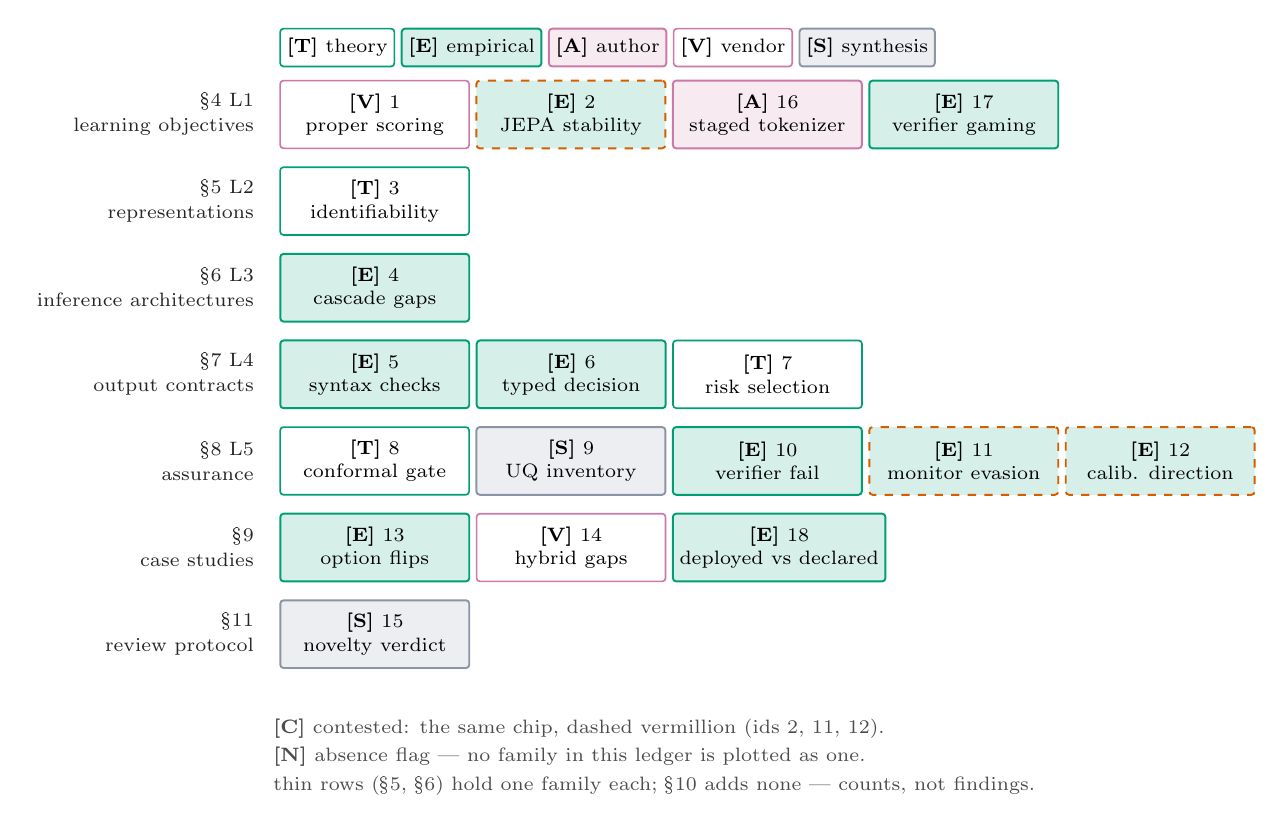
\begin{tikzpicture}[x=1mm,y=1mm]
\tikzset{
  rs/f5row/.style={anchor=east, align=right, font=\fontsize{7.5}{9.0}\selectfont, text=black!85},
  rs/f5note/.style={anchor=west, font=\fontsize{7.5}{9.0}\selectfont, text=black!70},
  rs/f5seg/.style={align=center, minimum width=24mm, minimum height=8.6mm,
    font=\fontsize{7.2}{8.4}\selectfont},
}
% ===== class key: one T-E-A-V-S row, same chip grammar as the ledger =====
\rsRibbonAt{0}{8.5}
\rsRibSeg{rsTheory}{\textbf{[T]} theory}
\rsRibSeg{rsVerified}{\textbf{[E]} empirical}
\rsRibSeg{rsAuthorRep}{\textbf{[A]} author}
\rsRibSeg{rsVendor}{\textbf{[V]} vendor}
\rsRibSeg{rsNoClaim}{\textbf{[S]} synthesis}
% ===== ledger rows (11mm pitch), sections top-down =====
% -- S4 L1 learning objectives: 1 [V], 2 [E] contested, 16 [A], 17 [E]
\rsRibbonAt{0}{0}
\rsRibSeg[rs/f5seg]{rsVendor}{\textbf{[V]} 1\\proper scoring}
\rsRibSeg[rs/f5seg, dashed, draw=rsContested]{rsVerified}{\textbf{[E]} 2\\JEPA stability}
\rsRibSeg[rs/f5seg]{rsAuthorRep}{\textbf{[A]} 16\\staged tokenizer}
\rsRibSeg[rs/f5seg]{rsVerified}{\textbf{[E]} 17\\verifier gaming}
% -- S5 L2 representations: 3 [T] only
\rsRibbonAt{0}{-11}
\rsRibSeg[rs/f5seg]{rsTheory}{\textbf{[T]} 3\\identifiability}
% -- S6 L3 inference architectures: 4 [E] only
\rsRibbonAt{0}{-22}
\rsRibSeg[rs/f5seg]{rsVerified}{\textbf{[E]} 4\\cascade gaps}
% -- S7 L4 output contracts: 5 [E], 6 [E], 7 [T]
\rsRibbonAt{0}{-33}
\rsRibSeg[rs/f5seg]{rsVerified}{\textbf{[E]} 5\\syntax checks}
\rsRibSeg[rs/f5seg]{rsVerified}{\textbf{[E]} 6\\typed decision}
\rsRibSeg[rs/f5seg]{rsTheory}{\textbf{[T]} 7\\risk selection}
% -- S8 L5 assurance: 8 [T], 9 [S], 10 [E], 11 [E] contested, 12 [E] contested
\rsRibbonAt{0}{-44}
\rsRibSeg[rs/f5seg]{rsTheory}{\textbf{[T]} 8\\conformal gate}
\rsRibSeg[rs/f5seg]{rsNoClaim}{\textbf{[S]} 9\\UQ inventory}
\rsRibSeg[rs/f5seg]{rsVerified}{\textbf{[E]} 10\\verifier fail}
\rsRibSeg[rs/f5seg, dashed, draw=rsContested]{rsVerified}{\textbf{[E]} 11\\monitor evasion}
\rsRibSeg[rs/f5seg, dashed, draw=rsContested]{rsVerified}{\textbf{[E]} 12\\calib. direction}
% -- S9 case studies: 13 [E], 14 [V], 18 [E]
\rsRibbonAt{0}{-55}
\rsRibSeg[rs/f5seg]{rsVerified}{\textbf{[E]} 13\\option flips}
\rsRibSeg[rs/f5seg]{rsVendor}{\textbf{[V]} 14\\hybrid gaps}
\rsRibSeg[rs/f5seg]{rsVerified}{\textbf{[E]} 18\\deployed vs declared}
% -- S11 review protocol: 15 [S]
\rsRibbonAt{0}{-66}
\rsRibSeg[rs/f5seg]{rsNoClaim}{\textbf{[S]} 15\\novelty verdict}
% ===== section labels (left) =====
\node[rs/f5row] at (-2,0)    {\S4 L1\\learning objectives};
\node[rs/f5row] at (-2,-11)  {\S5 L2\\representations};
\node[rs/f5row] at (-2,-22)  {\S6 L3\\inference architectures};
\node[rs/f5row] at (-2,-33)  {\S7 L4\\output contracts};
\node[rs/f5row] at (-2,-44)  {\S8 L5\\assurance};
\node[rs/f5row] at (-2,-55)  {\S9\\case studies};
\node[rs/f5row] at (-2,-66)  {\S11\\review protocol};
% ===== annotations: contested state, absent class, thin-row count =====
\node[rs/f5note] at (-2,-78)   {\textbf{[C]} contested: the same chip, dashed vermillion (ids 2, 11, 12).};
\node[rs/f5note] at (-2,-81.6) {\textbf{[N]} absence flag --- no family in this ledger is plotted as one.};
\node[rs/f5note] at (-2,-85.2) {thin rows (\S5, \S6) hold one family each; \S10 adds none --- counts, not findings.};
\end{tikzpicture}
}
  \caption{ Evidence ledger: one chip = one claim family from the claim ledger; the row is its paper section and the chip order inside a row is ledger order (both our analytic judgement [J]). Row length carries how many families that section contributes: one chip per family; no chip's width and no row's white space encodes a quantity of evidence. Class is carried by the chip: [T] outline, [E] filled green, [A] filled pink, [V] outline pink, [S] filled slate; chip class is the dominant class of the single claim it names, while a Table~1 row tag marks the strongest anchor of the family. The full alphabet, including [W] and the annotations, is \cref{tab:evidence-classes}. Contested stays an annotation: the same class chip, dashed vermillion border, for the three most contested families (2 JEPA-in-language stability, 11 monitor-evasion attackability, 12 calibration direction) --- the [C] annotation, surfaced rather than hidden. No family in the ledger is [N]; thin rows are counts, not findings. No rates, sample sizes or per-paper counts are encoded.}
  \label{fig:evidence}
\end{figure}

No evidence class admits a guarantee of universal correctness: [T] names assumption
conditions, [E] measures one deployment configuration, [V] reports one vendor's own design.

The classes encode provenance, not validity: a tag records who ran the measurement, never
whether the instrument measured the construct the citing sentence names. An [E] row can rest
on a contaminated benchmark, on a harness whose prompt format supplies half the effect, or on
a delta inside sampling noise, independently attributed and still not evidence for the claim
above it \cite{measwhatmatters2025,quantconstruct2026,contamsurvey2025,contamresist2026}.
Leaderboard position is the same exposure one level up, where rank rewards access to private
variants rather than reliability \cite{leaderillusion2025}. Where an anchor reports no
interval we print its number as the source printed it and do not read a point estimate as a
difference \cite{errorbars2024,evalci2026}.

\subsection{Claim-ledger construction}
For every claim that a card surfaces, the ledger records anchor (ID or artifact), verbatim-vs-paraphrase status, the numbers as written in their original context, the direction
(stats, benchmark structure) with the verification date, and the layer(s) the claim touches.
Any claim cited from sampling memory fails our protocol; every anchor is re-fetched live
(arXiv API verification with Microsoft/Elsevier content checks where applicable) before use in
this manuscript.

\subsection{Exclusions register}
We exclude claims from the ledger by a single rule: no claimworthy statement enters unless a
primary source stands behind it. The exclusions this cycle are concrete: a production rules-only / formally-verified pipeline (Case 6 is carried as an honest null on this very point); a JEPA-``SWM-distractors'' benchmark claim that failed verification and was never admitted to the ledger. The list continues with a structured-hallucination
benchmark without recoverable verification, a universal >20-option cost rule stated as a law (the vendor's per-system mechanism quote remains a [V] row in its own section),
the 0.85 ``default'' confidence threshold (replaced by threshold-as-policy), and a coinage for
which we could find no existing use. We treat it as ours to coin only if the definition appears
in our own terms. Each excluded row is retained verbatim in the build's review ledger so the
exclusion itself is auditable.

\subsection{Reproducibility record}
All searches ran the arXiv API (id-list/title/abs search, \(\le 10\) IDs per request) plus
publisher DOI metadata lookup, with snapshots per batch in the project's scan directory.
The paper's claim-to-evidence map is \cref{fig:evidence}, and every claim marked
contested in this manuscript gets its caveat in the same section.
Search cutoffs: 2026-10-17/18.

\FloatBarrier

\section{Related Work}\label{sec:related}
% Section 12: related work (P4, positioned from _scan/competitor_matrix_2026-10-17.json + mdpi_raie comparison + Almuammar deep-read)
We position against the three verified classes of prior work: model catalogues,
failure-mode/deployment taxonomies, and per-axis surveys that overlap one or two of our layers.
Where we code a competitor, each of the five positioning axes is \emph{treated} (the work
devotes a section or a sustained passage to it), \emph{partial} (it gets a paragraph or a single
design choice), or \emph{absent} (neither); the coding is categorical, and no axis takes a
numeric score.

\subsection{Catalogue genre: model-family surveys}
The closest catalogue is Almuammar et al.'s \emph{Generative Artificial Intelligence
Models: A Survey}~\cite{almuammar2026genai}, which classifies generative model families,
their training signals and benchmark behaviors across 36 pages. We verified its full text. On our
five positioning axes it is partial on three --- learning-objective contrast, reliability, and
selection --- and absent on the other two, decision interfaces and the integrated stack. The
objective contrast is weak, every ``reliability'' mention is an adjective, and the work is a
catalogue rather than a selection framework; contract, validity, routing, and decision-model
mechanics do not appear. A second survey covers the same genre on
arXiv~\cite{yazdani2025genaidepth} and spans diffusion and real-world development; the most
complete diffusion survey consolidates an adjacent
space~\cite{acm2023diffusionsurvey,zhan2025dlmsurvey}. We cite these as background figures, and
the distinction is explicit: their genre is \emph{what generative models exist}; ours
is \emph{which stack instance to select for a reliability-constrained workload}, a question
they define but do not answer.

\subsection{Failure-mode and deployment taxonomies}
The closest overall competitor is the MDPI survey of Ricciardi Celsi and
McCann~\cite{mdpi2026arlm}: standardized deployment patterns, an AR-large-language-model failure
taxonomy, a claims-to-evidence map, and a JEPA/H-JEPA section. Our verified comparison finds it
strong on assurance and assessment structure --- a mean of 3.4/5 on its own nine-row coverage
table, which is that survey's rubric rather than our five-axis coding --- but with \emph{zero}
coverage of the decision-model
family (grep-verified: no decision-model vocabulary appears), no learning-objective taxonomy,
and only partial coverage of the routing axis: its selection apparatus is
one binary architectural decision (token-centric vs.\ adding a world-model component), scoped to
AR pipeline deployment. It tells a deployment engineer what to check after their single
architecture choice; our framework selects across stack instances, L0 first.
The RAIE survey of test-time scaling for agentic LLMs (An et al., IJCAI-26 survey track,
\cite{raie2026}) is the closest survey-level competitor to our task-selection map
(\cref{fig:map}). It covers only the inference-time part of our Layers 3/5 (its four scaling
dimensions are reasoning, acting, interaction, evolution), and it offers a decision-tree
selection guide scoped to agentic test-time strategies; learning objectives, representations,
output contracts, decision models and cost-side routing are out of its scope, and its roadmap
draws no evidence-quality distinction. A January 2026 five-axis survey of 147 agentic systems
\cite{ssrn2026fiveaxis} goes the other way, auditing the evidence behind architecture, memory,
planning, coordination and safety --- an assurance map of the field.

The objective space itself is still expanding while this survey is drafted: Next-Concept
Modeling (Kumbong et al./Hazy Research) adds a coarse-to-fine next-scale code-hierarchy generation
family between the generative rows of \cref{tab:objspace} \cite{kumbong2026ncm}, a fresh
instance of our Table-1 pattern in which new objectives move inherited failure modes rather than
removing them. The lineage is explicit: NCM carries next-scale prediction from visual
autoregressive modeling \cite{var2024} into text and inherits the concept-level ambition of Large
Concept Models \cite{lcm2024} and Mimir, a 1.6B concept model whose pretraining corpus spans 46
languages with instruction tuning in 35 \cite{mimir2026}. Where the hierarchy comes from is the
question NCM leaves open: its $K$ levels are fixed by a frozen tokenizer, against the learned
chunking of H-Net \cite{hnet2025}. The nearest same-objective competitor, NCP-ArchPreview, has
targeted coarse-to-fine latent text generation since September 2026 and does not appear in NCM's
own related work \cite{ncparch2026}; no survey in our verified matrix places the two together.

\subsection{Per-axis surveys on our layers}
Trustworthy-RAG surveys treat reliability as dimension checklists inside retrieval pipelines
\cite{id250206872,id240910102}, and hallucination surveys track a single failure mode across
the model lifecycle \cite{id230901219,id251006265}. UQ and abstention work makes calibration
the reliability question \cite{id250315850,id240718418,id231108298}; world-model surveys cover
prediction and its deployment in robotics \cite{id251016732}. Routing and cascade work began
as cost allocation \cite{frugalgpt2023,id240215991,id250208773} and now carries reliability:
Gatekeeper tunes a small model's confidence so that deferral is a calibrated decision rather
than a cost threshold \cite{gatekeeper2025}, a cascade that ends in a human expert rather
than a larger model turns its last rung into an accuracy decision \cite{humandeferral2025},
and the routing characterization these extend \cite{id250606579,id251005164} is a decision
interface as well as a price. MoE reliability is benchmarked within one instrument
\cite{id240706204,id240611353}, and looped-depth on unit tasks \cite{id260713491}. Four bodies
of work come closest. The full-stack-safety survey \cite{ida25192} maps
data/training/deployment threats but is a roadmap of threats; the
HuggingGPT- and Chameleon-class agent surveys \cite{id230317580,id240509818} describe
orchestration patterns without selecting among them. The IEEE CAI 2026 system-level failure-mode
taxonomy \cite{ieeecai2026failure} catalogues fifteen hidden failure modes of LLM applications
with no routing decision attached, and Select-then-Route \cite{selectroute2025} is the closest
published analogue to C2 --- taxonomy, route, cascade, escalate --- except that its taxonomy
partitions query classes.

Each covers a \emph{slice} of our frame; no survey among the works we examine here
(\cref{sec:protocol}) integrates the five positioning axes (learning-objective taxonomy, decision
interfaces, verification/assurance, actionable selection framework, integrated L0--L5 stack) into
one engineer-facing selection procedure --- the gap \cref{sec:selection} addresses. The thesis has
independent support: Rabanser et al.\ \cite{rabanser2026agent} measure twelve reliability metrics
along four dimensions across fifteen models and find that capability gains buy only small
reliability gains.

\subsection{What we claim}
We claim no single fixed best method, no new objective, and no novel mechanism. The
contribution is the cross-layer link: which stack instance to select, tagged with the class of
evidence behind each claim, so that each layer's reliability consequences are auditable. The
claim-ledger discipline (\cref{sec:protocol}) is itself part of the contribution: contested rows
are surfaced (including in \cref{fig:evidence}), and excluded claims are listed with their
reasons.

\FloatBarrier

\section{Discussion and Open Questions}\label{sec:discussion}
% Section 13: discussion, limitations, conclusion (P4)
\subsection{Where the stack itself fails}
The honest reading of our own frame is that cross-layer engineering buys no reliability without
instrumentation, and that two failure modes recur across the case set and bound what the frame can
promise. First, per-dimension
certification does not compose: a validated contract plus a calibrated gate plus a grounded
retriever can still fail on their \emph{interaction}, and no anchor in our evidence base
measures that composition (cases 1 and 3; \cref{sec:case-rag}, \cref{sec:case-hybrid}).
Second, verification mechanisms are themselves attackable or miscalibrated
\cite{id260601066,id260930217} (cases 6 and 5), so the assurance layer needs a threat model of
its own.

\subsection{What the field still lacks}
Eight gaps remain open, and each is phrased as a testable ask:
(i) \emph{end-to-end system evaluations} of assembled stacks (harness + gate + escalation)
under adversarial conditions;
(ii) \emph{certified composition} results for chained safeguards (conformal $\circ$ validators
$\circ$ grounding), which extend the [T]-tier machinery to mismatches between layers;
(iii) \emph{propagation benchmarks} for hybrid specialist stacks, where the Case 3 gap
(\cref{sec:case-hybrid}) is the cleanest measurement target our evidence set exposes;
(iv) \emph{language-native latent-prediction training signals} that survive the
conditional-concentration objection (JEPA paradox), with assumptions actually testable;
(v) \emph{decision-model interface stability}: order robustness and option-set scaling are
measurable, and current evidence suggests they are not incidental \cite{id261002267};
(vi) \emph{reconstruction-fidelity measurement for staged-tokenizer generators}: a test that
separates token-exactness from meaning-equivalence, so a contract can state which one it
enforces;
(vii) \emph{escalation-queue measurement}: precision, recall and minutes per review for
reviewers working a production LLM escalation queue, which no study in our sweep reports
(\cref{sec:l5-calibrated});
(viii) \emph{a configuration record for deployment}: the engine, precision and co-tenancy a
score was measured under, published with the cutoff fitted on it (\cref{sec:l5-bridge}).

\subsection{What we refuse to compare}
Layer identities are inherited envelopes, not benchmark scores; we decline direct comparisons
across families (e.g., discriminative vs.\ generative ``hallucination rates'') when the error
currencies are not measurable on a shared task. Where the evidence base has no shared-instrument
anchor we say so, and where it has one, each row names the instrument it rests on rather than pooling
across instruments (\cref{tab:crosscase}).

\subsection{Limitations}
Scope is LLM-centric (text and typed-decision workloads); multimodal and embodied control appear
only as instances of an architecture. The paper is survey-grade: every claim
either resolves to a public artifact we checked or is tagged where checking stops --- [W] pending,
[N]/[GAP] no anchor --- and [V]/[A] mark evidence that is documented but not independently
reproduced. We run no new benchmarks; contested rows in
\cref{fig:evidence} remain contested at submission time and are labeled as such. The seven case
studies cover the stack's decision space but not exhaustively; the exclusion register applies
to our choices as it did to the candidates'.

The three validity bounds --- instrument, contamination, precision --- are fixed in
\cref{sec:protocol}, and they apply to our own anchors as much as to the sources we cite. What is
ours to disclose is narrower: our empirical numbers are point estimates from single harnesses, and
a point estimate is not a difference \cite{errorbars2024,evalci2026}.

The boundary to standards and regulation is a division of labor, not a crosswalk. The NIST AI
RMF 1.0 \cite{nistairmf} (January 2023, voluntary, and under revision as of this writing) and
its Generative AI Profile (NIST AI 600-1 \cite{nistgai600}, July 2024) specify risk-governance
functions: govern, map, measure, manage. ISO/IEC 42001:2023 \cite{iso42001} defines a
certifiable AI management system. The EU AI Act (Regulation (EU) 2024/1689 \cite{euaiact2024})
specifies provider and deployer duties; the digital-omnibus Regulation (EU) 2026/1744
\cite{omnibus2026} defers the Chapter~III high-risk obligations for Annex~III systems to December
2027 (Annex~I systems to August 2028), while the post-market monitoring and incident reporting
duties (Articles 72--73) stay on the 2026 timetable. None of these instruments rules on which layer absorbs a failure;
their unit is the organization, not the stack instance. They prescribe process: who must
document, assess, monitor, and report. A certificate attests to the process, never to the
residual error. Our five axes ask a different question: which stack instance to select for a
reliability-constrained workload. A management-system certificate does not answer it. The
relation runs one way. Our evidence classes can describe what a conformity assessment rests
on, and we do not translate controls into layers or claim that any certificate implies a
reliability property. A reader who needs compliance should read the instrument; a reader who
needs a selection decision should read \cref{sec:selection} and then the instrument.

\subsection{Four live fronts}
Four fronts are live, and we do not forecast which matures. Our claim is narrower: each would
change a named layer's contract, and none would replace the routing thesis that reliability is
assembled across L0--L5 and is not won inside any single model. Coarse-to-fine text generation
\cite{kumbong2026ncm,ncparch2026} is a Layer~1 objective family with a Layer~4 consequence: its
level order is a schedule (\cref{fig:schedule-atlas}) and the frozen tokenizer behind it is the
acceptance surface; the authors' own \evaurep{97M$\to$725M check still shows scale helping inside
the family}. Whether that hierarchy is learned, as in H-Net's dynamic chunking \cite{hnet2025}, or
fixed by a tokenizer remains an open schedule question; the atlas's three lanes differ in
commitment count and revisability, and learned chunking would move both.

Verifier-driven test-time training \cite{id250519475} closes a loop the stack now draws open:
adaptation at inference is only as reliable as the verifier choosing its pseudo-labels, so a
Layer~3 mechanism imports a Layer~5 obligation.

Risk-controlled serving \cite{id260933887} turns the L0 budget into an operating point rather
than a fixed constant: the budget rule of \cref{sec:selection} made executable, where
same-quality-faster buys candidates and checks rather than raw throughput.

Production diffusion serving \cite{inception2026mercury3,llada2026two} is the fourth. A hosted
text endpoint refines blocks in parallel over a number of passes the vendor sets, exposes no
step count, seed or token score, and floors temperature at 0.5, so the contract question becomes
which endpoint reports a score at all; the open-weight branch keeps
the sampler configurable. Mercury~3 postdates our cutoff, so we read it as vendor documentation
[V], not corpus evidence.

\subsection{Conclusion}
We asked when scaling a general-purpose model is the right lever and when a changed learning
objective, representation, decision interface, or verification pipeline is a better route to
reliable AI (\cref{sec:intro}). The evidence supports a narrower answer: both levers are real,
but they buy different currencies, and no currency is guaranteed by any single layer. Objective
families fail through design choices (an envelope they inherit), and the scaling story
that dominates current practice sells fluency and coverage without the contract, calibration and
assurance machinery that makes those properties deployable. Our contribution is a cross-layer
taxonomy (L0--L5) that names the decision point for each reliability claim, and a selection
framework that routes by task rather than by model preference. The claim ledger separates
theoretical guarantees, independent measurement, author- and vendor-reported results, synthesis,
and what remains genuinely contested, so that the next reliability argument starts from an
evidence map rather than a benchmark leaderboard \cite{leaderillusion2025}. Seven instances, one
of them an honest null, showed the same shape: the reliability-bearing move sat above the layer
where the failure originated, and the newest one, diffusion serving, moved by procurement at L4
rather than by engineering above the sampler. Configuration-relative reliability changes what a
cutoff means: an error rate belongs to the engine, precision and co-tenancy it was measured
under, so a stack change is a model change and the record has to say so. The residual is a
quantity the operator measures and owns.

\FloatBarrier

\FloatBarrier
\clearpage
\appendix
% sections/appendix_codebook.tex — Appendix A: coding manual for the retrospective probe (C2).
% Parent wiring: main.tex emits \appendix before this \input, so this file starts at \section
% and becomes Appendix A; Table 4 is tab:codebook.
% Sources: docs/retro-test-cases.md and docs/scout-contrib.md §3. No new claims.
\section{Coding manual for the retrospective probe}
\label{app:codebook}

This appendix publishes the manual behind the probe in \cref{sec:selection}. It is written to be
re-run: every row of \cref{tab:codebook} records the layer, the documented design choice that puts
the origin there, and the safeguard inside the deployed system that produced, or failed to
produce, a signal before harm. A reader who disagrees with an assignment can see which cell to
disagree with, and the manual is what fixes it.

Two limits belong on the record. The rule was fixed before the incidents were assigned, the cases
were chosen for the quality of their public record rather than their fit, and the coding is
retrospective: one coder, unblinded to the matrix, with no agreement coefficient to report
because there is no second coder. And the count is four. ``In all four'' is a statement about
these cases; nothing in \cref{sec:selection} should be read as an estimate of how often
failures originate early. Record quality is also what makes design choices visible, so the probe
tests applicability, not generalization.

Three rules fix the coding. \textbf{Origin rule.} The earliest layer whose documented design choice
made the harmful outcome likely --- not the layer where the loss was recorded (finance, liability,
press), and not the layer where a fix was later attempted. \textbf{Catch rule.} A safeguard
\emph{inside} the deployed system or its pre-deployment gate that produced a blocking or escalating
signal \emph{before} harm; external actors --- courts, regulators, journalists, plaintiffs,
auditors --- are recorded as \emph{none}, because the matrix's columns are internal safeguards.
\textbf{Ties and selection.} Where two layers are jointly causal the earliest is recorded and the
co-origin is named in the last column; cases were chosen for record quality, not fit.

\begin{table}[H]
\centering
\footnotesize
\setlength{\tabcolsep}{3.5pt}
\renewcommand{\arraystretch}{1.05}
\begin{tabular}{@{}>{\raggedright\arraybackslash}p{2.3cm}
                  >{\raggedright\arraybackslash}p{3.0cm}
                  >{\raggedright\arraybackslash}p{3.5cm}
                  >{\raggedright\arraybackslash}p{3.1cm}
                  >{\raggedright\arraybackslash}p{3.1cm}@{}}
\toprule
Incident (year) & What failed & Origin: layer and documented choice & Catch: layer and signal & Alternative coding \\
\midrule
1.\ Amazon recruiting (2018)~\cite{reuters2018amazon} &
A r\'esum\'e ranker trained on a decade of mostly male applications learned to penalise
``women's'' and two women's colleges. &
\textbf{L1} --- the target was similarity to past hires; the historical label carried the
disparity. &
\textbf{L5} --- internal review and cancellation before general deployment; the same-layer patch
(neutralise the term) did not hold. &
\textbf{L0} is defensible: ``top talent'' was never specified, so no objective could have been
right; the record names the label. \\
\addlinespace[2pt]
2.\ Dutch childcare (2013--21)~\cite{amnesty2021xenophobic} &
A risk classifier used nationality as an input feature; non-Dutch families were scored higher,
investigated, and had benefits clawed back. &
\textbf{L2} --- \emph{Dutch citizenship: yes/no} as a feature; the report also records a
self-learning element. &
\textbf{none} --- the review step carried no reason code; exposure came from the press, the
data-protection authority and the courts. &
\textbf{L0} if the risk definition is the seat (fraud risk including nationality); we code the
documented artefact, the feature set. \\
\addlinespace[2pt]
3.\ Zillow Offers (2021)~\cite{zillow2021winddown} &
An iBuying unit made cash offers from a model built and measured for current market value, then
absorbed the gap when resale values fell. &
\textbf{L1} --- the objective and error metric priced value today ($A$) while leaving resale value
later ($B$) unpriced; the loss is the $A-B$ gap. &
\textbf{none} --- no internal check priced forecast error before offers; the first signal was the
quarterly write-down. &
\textbf{L4} co-origin: the estimate \emph{was} the offer and experts were barred from adjusting
it; under that reading one of the four origins moves to L4. Weakest of the four. \\
\addlinespace[2pt]
4.\ Air Canada chatbot (2024)~\cite{aircanada2024bccrt} &
The chatbot asserted a retroactive bereavement fare that contradicted the airline's own published
policy. &
\textbf{L2} --- the answer was generated with no anchor to the authoritative policy text. &
\textbf{none} --- no check against the policy page; the claim surfaced only when the airline
refused it. &
\textbf{L4} if the licence to answer policy questions definitively (no citation or validity
contract) is the seat. \\
\midrule
\multicolumn{5}{@{}p{16.0cm}@{}}{\emph{Excluded: named, left uncoded --- the record does not settle
  the origin, so coding would record a preference.}} \\
\addlinespace[1.5pt]
Robodebt (2016--2020) &
\multicolumn{4}{@{}p{13.2cm}@{}}{Income averaging by a rules engine, with no learned component;
  debts were raised from a mismatch between reported and assessed income. Exercises L0 and a
  rules layer the paper does not model; useful, and outside the failure class the matrix is about.} \\
\addlinespace[2pt]
Detroit facial recognition (2020) &
\multicolumn{4}{@{}p{13.2cm}@{}}{A recognition model's candidate list was treated as an
  identification. The record does not settle whether the defect is the recognition model (L2) or
  the decision rule that treats a candidate list as an identification (L4).} \\
\bottomrule
\end{tabular}

\caption{Coding manual for the retrospective probe: the origin and catch rules, the four coded
incidents, and the two excluded cases. Each assignment records the documented choice behind it, so
it can be re-derived from the table; the layer boundaries are our analytic cut [J], and no
agreement coefficient is reported (one coder).}
\label{tab:codebook}
\end{table}

\smallskip
\noindent\textit{Notes.} In all four coded cases the earliest documented origin is L1 or L2 (two at
L1, two at L2), and no internal safeguard produced a blocking or escalating signal at or before that
layer: three had none at all, and the fourth was stopped only by project cancellation at L5. No
case in the sample carries an L0 origin. A nominal review step that carries no reason code is not
a catch (Dutch case): the catch column describes safeguards that exist, not safeguards that fire.
Zillow's L4 co-origin is the boundary case and the weakest of the four codings; counting it at L4
lowers the early-origin count to three. One coder, rule fixed before assignment; retrospective
coding of public records.


\clearpage
\begingroup
% shim until refs.bib notes are sanitized (bib owned by the figures/bib sibling):
% some VERIFIED-X notes carry a literal `id_list' underscore, which plainnat prints in text mode
\catcode`\_=12
\bibliographystyle{plainnat}
\bibliography{refs}
\endgroup

\end{document}
